\documentclass[12pt, a4paper]{article}

% ── Packages ──────────────────────────────────────────────────────────────────
\usepackage[a4paper, margin=2.5cm]{geometry}
\usepackage{graphicx}
\usepackage{float}
\usepackage{amsmath}
\usepackage{amssymb}
\usepackage{xcolor}
\usepackage{mdframed}
\usepackage{parskip}
\usepackage{enumitem}
\usepackage{titlesec}
\usepackage{booktabs}
\usepackage{tikz}
\usepackage{hyperref}
\usepackage[T1]{fontenc}

% ── Graphics path ─────────────────────────────────────────────────────────────
\graphicspath{{../../Images_for_latex/Lecture_11/}}

% ── Colours ───────────────────────────────────────────────────────────────────
\definecolor{keyblue}{RGB}{30, 80, 160}
\definecolor{keybluebg}{RGB}{220, 235, 255}
\definecolor{noteorange}{RGB}{200, 100, 0}
\definecolor{noteorangebg}{RGB}{255, 240, 215}
\definecolor{warnred}{RGB}{180, 30, 30}
\definecolor{warnredbg}{RGB}{255, 220, 220}
\definecolor{defgreen}{RGB}{20, 110, 50}
\definecolor{defgreenbg}{RGB}{215, 245, 225}
\definecolor{headernavy}{RGB}{25, 35, 90}

% ── Box environments ──────────────────────────────────────────────────────────
\newmdenv[linecolor=keyblue,backgroundcolor=keybluebg,linewidth=1.5pt,
  leftline=true,rightline=false,topline=false,bottomline=false,
  innerleftmargin=10pt,innerrightmargin=8pt,
  innertopmargin=6pt,innerbottommargin=6pt,
  skipabove=8pt,skipbelow=8pt]{keybox}

\newmdenv[linecolor=noteorange,backgroundcolor=noteorangebg,linewidth=1.5pt,
  leftline=true,rightline=false,topline=false,bottomline=false,
  innerleftmargin=10pt,innerrightmargin=8pt,
  innertopmargin=6pt,innerbottommargin=6pt,
  skipabove=8pt,skipbelow=8pt]{notebox}

\newmdenv[linecolor=warnred,backgroundcolor=warnredbg,linewidth=1.5pt,
  leftline=true,rightline=false,topline=false,bottomline=false,
  innerleftmargin=10pt,innerrightmargin=8pt,
  innertopmargin=6pt,innerbottommargin=6pt,
  skipabove=8pt,skipbelow=8pt]{warnbox}

\newmdenv[linecolor=defgreen,backgroundcolor=defgreenbg,linewidth=1.5pt,
  leftline=true,rightline=false,topline=false,bottomline=false,
  innerleftmargin=10pt,innerrightmargin=8pt,
  innertopmargin=6pt,innerbottommargin=6pt,
  skipabove=8pt,skipbelow=8pt]{defbox}

% ── Section formatting ────────────────────────────────────────────────────────
\titleformat{\section}[block]{\large\bfseries\color{headernavy}}{}{0pt}{}
  [\vspace{2pt}\rule{\linewidth}{0.8pt}\vspace{4pt}]
\titleformat{\subsection}[block]{\normalsize\bfseries\color{keyblue}}{}{0pt}{}

% ── Document ──────────────────────────────────────────────────────────────────
\begin{document}

\begin{center}
  {\LARGE\bfseries\color{headernavy} Sensors \& Systems}\\[4pt]
  {\large Sensor Fusion}\\[2pt]
  {\normalsize Jan Bendtsen, Torben Knudsen \quad|\quad Electronic Systems, 8th Semester}
\end{center}

\vspace{4pt}\hrule height 1.2pt\vspace{12pt}

% ==============================================================================
\section*{Section 1 \quad What is Sensor Fusion?}
% ==============================================================================

% ------------------------------------------------------------------------------
\subsection*{1.1 \quad Simple Sensors --- A Starting Point}
% ------------------------------------------------------------------------------

\begin{figure}[H]
  \centering
  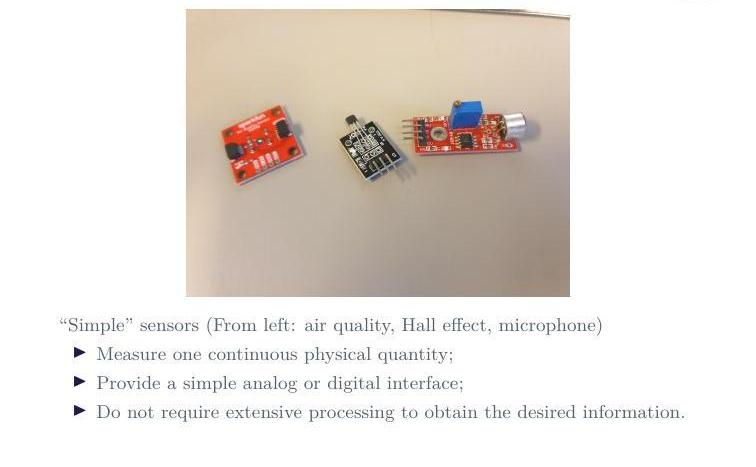
\includegraphics[width=\textwidth]{slide-03.jpg}
  \caption{Three examples of ``simple'' sensors used throughout the course.
    From left: an \textbf{air quality sensor} (measures a single gas
    concentration), a \textbf{Hall effect sensor} (detects the presence and
    strength of a magnetic field), and a \textbf{microphone} (measures acoustic
    pressure as a voltage).
    Each device outputs \emph{one} continuous physical quantity via a simple
    analog or digital interface.}
\end{figure}

Throughout this course we have built up the theory of state estimation ---
Kalman filters, EKF, UKF --- largely in the context of a single sensor
measuring a single physical quantity.
Recall the defining properties of a ``simple'' sensor:

\begin{itemize}[leftmargin=1.4em, itemsep=3pt]
  \item \textbf{Measures one continuous physical quantity} --- one number out
    per sample (temperature, pressure, light intensity, magnetic field strength,
    etc.).
  \item \textbf{Provides a simple analog or digital interface} --- the output
    is directly readable as a voltage, a current, or a digital word.
    No significant onboard processing is needed.
  \item \textbf{Does not require extensive processing to obtain the desired
    information} --- the measured quantity is already close to what the
    application needs.
    A microphone gives you the sound pressure; you do not need to do
    much more to know how loud something is.
\end{itemize}

\begin{notebox}
  \textbf{Why ``simple'' sensors are not always sufficient}

  Simple sensors have two fundamental weaknesses that motivate sensor fusion:

  \begin{itemize}[leftmargin=1.2em, itemsep=3pt]
    \item \textbf{Each sensor measures something slightly different from what
      you ultimately want.}
      A gyroscope measures \emph{angular rate}; you want \emph{orientation}.
      A GPS receiver measures \emph{position} but is noisy; an
      accelerometer measures \emph{acceleration} but drifts.
      No single sensor gives you what you want, cleanly and completely.

    \item \textbf{Each sensor has its own noise, bias, and blind spots.}
      A gyroscope drifts over time (integrating a small bias error builds up
      into a large orientation error).
      A magnetometer is accurate in steady state but disturbed by nearby metal.
      An accelerometer cannot distinguish gravity from linear acceleration.
      These weaknesses are different for each sensor --- which means they
      can complement each other if combined correctly.
  \end{itemize}

  The idea of sensor fusion is to use several sensors at once so that the
  strengths of each compensate for the weaknesses of the others.
  The remaining sections of this lecture develop three concrete frameworks for
  doing this: the Kalman filter (Section~2), the complementary filter
  (Section~3), and the Madgwick/Mahoney filters for attitude estimation
  (Sections~4--7).
\end{notebox}

% ------------------------------------------------------------------------------
\subsection*{1.2 \quad Sensor Fusion --- Definition and Goal}
% ------------------------------------------------------------------------------

\begin{figure}[H]
  \centering
  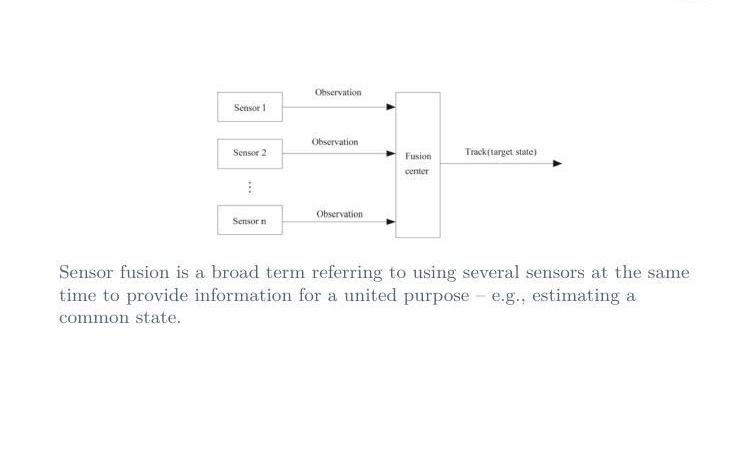
\includegraphics[width=\textwidth]{slide-04.jpg}
  \caption{General sensor fusion architecture.
    Each of $n$ sensors produces an \textbf{observation} (a noisy measurement
    of some aspect of the environment or system state).
    All observations are fed into a central \textbf{fusion centre}, which
    combines them to produce a single estimate of the \textbf{track} or
    \textbf{target state} --- the quantity we actually care about.
    The arrows indicate that information flows \emph{from} the sensors
    \emph{to} the fusion centre, not the other way around: the sensors do not
    communicate with each other, only with the central estimator.}
\end{figure}

\textbf{Sensor fusion} is a broad term referring to the use of several sensors
simultaneously to provide information for a united purpose --- most commonly,
to estimate a shared underlying \emph{state}.

The key word is \textbf{state}: sensor fusion is not simply about collecting
more data.
It is about combining multiple imperfect windows onto the same underlying
physical reality to build a better estimate of that reality than any single
window could provide.

\begin{notebox}
  \textbf{What ``estimating a common state'' means --- a concrete example}

  Suppose you want to know the \emph{position and velocity} of a drone in
  3D space.
  This is the \textbf{state}: the vector $[x,\, y,\, z,\, v_x,\, v_y,\,
  v_z]^\top$ that fully describes where the drone is and how fast it is moving
  at a given moment.

  Now consider what individual sensors see:
  \begin{itemize}[leftmargin=1.2em, itemsep=2pt]
    \item \textbf{GPS} gives you $(x, y, z)$ --- position only, updated at
      1--10\,Hz, with errors of several metres.
    \item \textbf{Accelerometer} gives you $(a_x, a_y, a_z)$ --- the sum of
      linear acceleration and gravity, updated at $\sim$1000\,Hz, but drifts
      when integrated to position.
    \item \textbf{Barometer} gives you altitude $z$ --- slowly but steadily.
    \item \textbf{Camera} gives you optical flow --- velocity relative to what
      the camera sees.
  \end{itemize}
  None of these directly gives the full state at the required accuracy and
  update rate.
  But together, fed into a fusion centre (e.g.\ a Kalman filter), they
  produce a position and velocity estimate that is better than any of them
  individually.

  That is sensor fusion: the state $[x, y, z, v_x, v_y, v_z]^\top$ is the
  common thread; each sensor provides a noisy, partial view of it; the fusion
  centre combines all views into the best possible estimate.
\end{notebox}

\begin{notebox}
  \textbf{What makes one fusion approach better than another?}

  The fusion centre in the block diagram above is a placeholder.
  In reality it can be implemented in several ways, each with different
  assumptions and trade-offs:

  \begin{itemize}[leftmargin=1.2em, itemsep=3pt]
    \item \textbf{Kalman filter} (Section~2): optimal when the system dynamics
      are linear and all noise is Gaussian.
      Gives the minimum-variance state estimate.
      Naturally handles multiple sensors with a single unified framework.

    \item \textbf{Complementary filter} (Section~3): a simpler, frequency-domain
      approach that splits the measurement bandwidth between sensors.
      Computationally cheap and robust, but less general than the KF.

    \item \textbf{Madgwick / Mahoney filters} (Sections~6--7): nonlinear filters
      specifically designed for attitude estimation from IMU data.
      They exploit the geometry of rotations (quaternions) and are very
      efficient to run on embedded hardware.
  \end{itemize}

  All three frameworks appear in this lecture.
  They differ in complexity, generality, and computational cost, but they all
  serve the same purpose: combining imperfect observations into one good
  estimate of the state.
\end{notebox}

% ------------------------------------------------------------------------------
\subsection*{1.3 \quad Sensor Fusion for Decision Making}
% ------------------------------------------------------------------------------

\begin{figure}[H]
  \centering
  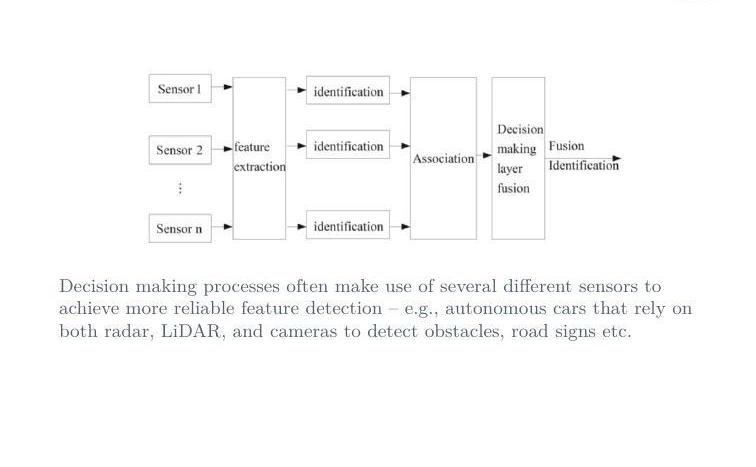
\includegraphics[width=\textwidth]{slide-05.jpg}
  \caption{Sensor fusion pipeline for \textbf{decision making}.
    Each sensor's raw output first passes through \textbf{feature extraction}
    (pulling out relevant descriptors from the raw signal) and then its own
    \textbf{identification} stage (classifying what those features correspond
    to --- a pedestrian, a road sign, a vehicle).
    The labelled detections from all sensors are then \textbf{associated}
    (matching detections across sensors that refer to the same real-world
    object), before the \textbf{decision making layer} combines the evidence
    into one agreed-upon classification that drives the system's action.}
\end{figure}

This is a fundamentally different use of sensor fusion from state estimation.
In state estimation (Section~2), you have a \emph{known physical state} ---
position, velocity, orientation --- and each sensor gives you a noisy
measurement of that same quantity.
The mathematics then tells you how to weight and combine those measurements
optimally.

Here that is not the case at all.
\textbf{Decision-making fusion} is about having several sensors that each form
their own \emph{independent opinion} about what is in the scene, and then
making the sensors \textbf{agree} on a final answer.
There is no state vector, no Kalman gain, no covariance matrix.
Each sensor does its own full processing pipeline ---
feature extraction, identification, classification ---
and arrives at a symbolic label
(``pedestrian with 87\% confidence'', ``road sign'', ``car'').
The fusion step then takes all those labels and resolves them into one
committed decision.

A canonical example is the \textbf{autonomous car}:
\begin{itemize}[leftmargin=1.4em, itemsep=3pt]
  \item \textbf{Radar} processes its echo returns and concludes:
    ``moving object, 30\,m ahead, radial velocity 1.2\,m/s.''
    It cannot tell whether it is a pedestrian or a large cardboard box.
  \item \textbf{LiDAR} processes its point cloud and concludes:
    ``upright shape, roughly human proportions, 30\,m ahead.''
    It cannot confirm the object is actually moving toward the road.
  \item \textbf{Camera} processes its image and concludes:
    ``pedestrian bounding box detected, 90\% confidence, at this pixel
    location.''
    It has no direct range measurement.
\end{itemize}

Each sensor arrives at its own answer independently.
The \textbf{association} step then asks: do the radar's ``moving object at
30\,m'', the LiDAR's ``human shape at 30\,m'', and the camera's ``pedestrian
at this pixel'' all refer to the same real object?
If yes, the \textbf{fusion identification} step combines the three independent
opinions into one: ``pedestrian confirmed, 30\,m ahead, moving 1.2\,m/s.''
This combined verdict is far more reliable than any single sensor could
produce, because the sensors would all have to make the same error
simultaneously to produce a false positive --- and since they use different
physical principles, their errors are \emph{independent}.

\begin{notebox}
  \textbf{Why this is ``agreeing'' and not ``averaging''}

  In state estimation fusion, you literally compute a weighted average of
  measurements.
  If GPS says you are at 57.00\,°N and another sensor says 57.02\,°N,
  the fused answer is somewhere between the two, weighted by each sensor's
  reliability.
  You combine \emph{numbers} about the \emph{same physical quantity}.

  In decision-making fusion you cannot do that.
  A radar range of 30\,m and a camera pixel coordinate of $(320, 240)$
  are not two noisy measurements of the same thing --- they are different
  types of information from different physical principles.
  There is no sensible way to ``average'' them.

  Instead each sensor produces a \emph{vote}: ``I believe there is a
  pedestrian.''
  The fusion layer then decides whether the sensors agree enough to commit
  to that decision.
  If radar says ``something is there'' and LiDAR says ``human-shaped''
  and the camera says ``pedestrian'', all three votes point the same way
  and the system acts on it.
  If only the camera fires and the others see nothing, the system may
  withhold the decision until it has more evidence.

  This is fundamentally a \textbf{consensus problem}, not an estimation
  problem.
  The tools used --- voting rules, Dempster-Shafer theory, Bayesian
  classifiers, neural network ensembles --- are different from the Kalman
  filter, and the result is a \emph{label} or \emph{decision}, not a state
  estimate with a covariance.
\end{notebox}

\begin{notebox}
  \textbf{Why independent sensor errors make fusion so powerful here}

  The key reason to fuse sensors in a decision pipeline is that their
  failure modes are \textbf{independent}:
  \begin{itemize}[leftmargin=1.2em, itemsep=2pt]
    \item Heavy rain scatters the LiDAR beam --- but the radar penetrates
      rain effortlessly.
    \item Darkness blinds the camera --- but LiDAR and radar are unaffected.
    \item A mirrored surface confuses LiDAR (returns go away from the
      sensor) --- but the camera can still read a sign on that surface.
  \end{itemize}
  For the system to make a \emph{wrong} decision, all the sensors that
  disagree must all fail in the same direction at the same moment.
  The probability of that is the product of the individual failure
  probabilities --- which is much smaller than any single sensor's failure
  probability.
  This is the core reliability argument for multi-sensor decision systems.
\end{notebox}

% ------------------------------------------------------------------------------
\subsection*{1.4 \quad Image Fusion --- A Concrete Decision-Making Example}
% ------------------------------------------------------------------------------

\begin{figure}[H]
  \centering
  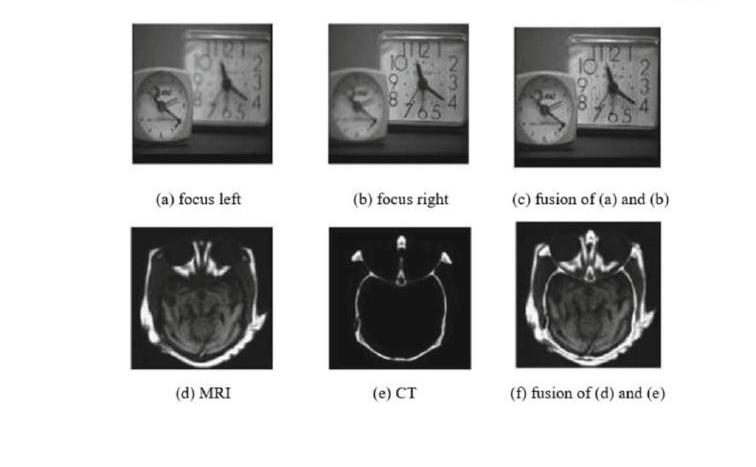
\includegraphics[width=\textwidth]{slide-06.jpg}
  \caption{Two examples of image-level sensor fusion.
    \textbf{Top row}: optical focus fusion.
    (a) An image focused on the \emph{left} clock --- the right clock is
    blurred.
    (b) An image focused on the \emph{right} clock --- the left clock is
    blurred.
    (c) A fusion of (a) and (b) --- both clocks are sharp simultaneously.
    No single camera position or focus setting achieves this; only fusing
    two images with complementary sharp regions produces the result.
    \textbf{Bottom row}: medical imaging fusion.
    (d)~\textbf{MRI} image: excellent soft-tissue contrast (shows internal
    organs and neural structures), but poor bone visibility.
    (e)~\textbf{CT} image: excellent bone and dense-structure contrast,
    but less soft-tissue detail.
    (f) Fusion of (d) and (e): both soft tissue and bone structure are
    visible simultaneously, giving the clinician more information than
    either modality alone.}
\end{figure}

Image fusion makes the complementary-sensor concept visually intuitive.
In both examples, no single sensor can capture everything:

\textbf{Optical focus fusion} exploits a fundamental limitation of any
lens-based imaging system: a camera can only be sharply focused at one
distance at a time.
Objects closer or further than the focal plane appear blurred.
By taking two images with different focal distances and fusing them ---
keeping only the sharp regions from each --- one obtains a single image
where everything is in focus.
This is the same complementary principle as the complementary filter of
Section~3: each sensor (each image) contributes what it is best at
(its in-focus region), and the fusion discards the rest.

\textbf{MRI + CT fusion} illustrates complementary physics:
\begin{itemize}[leftmargin=1.4em, itemsep=2pt]
  \item \textbf{MRI} (Magnetic Resonance Imaging) uses strong magnetic
    fields and radio waves to image the way hydrogen nuclei in water and fat
    relax.
    Tissues rich in water (brain, muscle, soft organs) give strong MRI signal;
    dense bone contains little free water and gives a weak signal.
    MRI is therefore excellent for soft tissue but poor for bone.
  \item \textbf{CT} (Computed Tomography) uses X-rays, which are absorbed
    in proportion to tissue density.
    Dense bone absorbs X-rays strongly and appears bright; soft tissue absorbs
    little and appears grey.
    CT is excellent for bone and dense structures but has lower soft-tissue
    contrast than MRI.
\end{itemize}
The two modalities are physically \emph{complementary}: each sees what the
other misses.
Their errors are also independent --- metal implants create artefacts in MRI
but are visible on CT; fluid-filled cavities appear clearly on MRI but can
be ambiguous on CT.
Fusing both images gives the clinician information that would otherwise require
two separate examinations.

\begin{warnbox}
  \textbf{Image fusion is harder than it looks --- the registration problem}

  Before any pixel-level fusion can happen, the two images must be
  \textbf{registered}: they must be aligned so that each pixel in image~(a)
  corresponds to the same physical location in image~(b).

  For the focus example this is trivial: the camera does not move between
  shots, so the pixels already align.
  For MRI + CT it is a major unsolved engineering challenge:
  \begin{itemize}[leftmargin=1.2em, itemsep=2pt]
    \item The patient may move slightly between scans.
    \item The two machines have different geometric distortions and
      resolutions.
    \item MRI and CT are acquired at different times and may show
      different tissue states (e.g.\ bladder fill level).
  \end{itemize}
  Registration is typically done by finding a rigid-body or non-rigid
  transformation (translation, rotation, scaling, warping) that maximises
  some measure of similarity between the two images.
  Only after registration is the pixel-level fusion meaningful.
  This is an example of the \textbf{data association problem} from
  Section~1.3 --- here at the pixel level rather than the object level.
\end{warnbox}

\begin{notebox}
  \textbf{Why these image examples are relevant to the rest of the lecture}

  The two image fusion examples are not just illustrations --- they encode
  the two fundamental reasons to fuse sensors that appear throughout this
  lecture:

  \textbf{Reason 1: The same thing, measured twice, more accurately.}
  The focus fusion example fuses two images of \emph{the same scene}.
  Neither image is wrong --- they are both correct pictures of the same
  reality, just with different blind spots (out-of-focus regions).
  Fusing them reduces those blind spots.
  This is the same motivation as the Kalman filter for sensor fusion
  (Section~2): both sensors measure the same state, each with its own noise,
  and combining them gives a better estimate than either alone.

  \textbf{Reason 2: Two different things, each inaccessible to the other
  sensor.}
  The MRI + CT example fuses two images that capture \emph{physically
  different} aspects of the same patient.
  Each image contains information the other cannot --- they are genuinely
  complementary.
  This is the same motivation as the complementary filter (Section~3) and
  the IMU fusion in Sections~4--7: the gyroscope sees high-frequency
  orientation changes that the accelerometer cannot track cleanly; the
  accelerometer sees the absolute gravity direction that the gyroscope
  cannot maintain over time.
  Both are needed.
\end{notebox}

% ── Key takeaways ─────────────────────────────────────────────────────────────
\begin{keybox}
  \textbf{Section 1 --- Key Takeaways}
  \begin{itemize}[leftmargin=1.2em, itemsep=2pt]
    \item \textbf{Simple sensors} each measure one physical quantity via a
      simple interface and require minimal processing.
      They are individually limited by noise, drift, and blind spots.

    \item \textbf{Sensor fusion} uses several sensors simultaneously to
      estimate a common state or make a joint decision, exploiting the fact
      that different sensors fail in different ways.

    \item There are two distinct fusion paradigms:
      \begin{itemize}[leftmargin=1.2em, itemsep=1pt]
        \item \textbf{State estimation fusion}: raw measurements combined at
          the signal level to estimate a shared physical state
          (e.g.\ Kalman filter, complementary filter).
        \item \textbf{Decision making fusion}: each sensor independently
          extracts features and classifies objects; the high-level symbolic
          outputs are then combined (e.g.\ autonomous car perception pipeline).
      \end{itemize}

    \item Sensors are most valuable when they are \textbf{complementary}:
      each sensor's weaknesses are covered by the others' strengths, and their
      noise sources are independent so errors do not compound.

    \item The image fusion examples illustrate both paradigms:
      focus fusion (same scene, reduce blind spots) mirrors the multi-sensor
      Kalman filter; MRI+CT fusion (different physical information) mirrors the
      complementary filter and IMU fusion in later sections.
  \end{itemize}
\end{keybox}

% ==============================================================================
\newpage
\section*{Section 2 \quad Kalman Filter for Sensor Fusion}
% ==============================================================================

We now turn to the state-estimation flavour of sensor fusion: multiple sensors
all measuring aspects of the \emph{same physical state}, combined inside a
single Kalman filter.
The good news is that the standard KF theory from earlier lectures carries over
almost unchanged --- the only new wrinkle is that several sensors may have
\emph{correlated} noise between them, which we need to handle before the
standard update equations can be applied.
This section develops that machinery step by step.

% ------------------------------------------------------------------------------
\subsection*{2.1 \quad The Multi-Sensor Discrete-Time Model}
% ------------------------------------------------------------------------------

\begin{figure}[H]
  \centering
  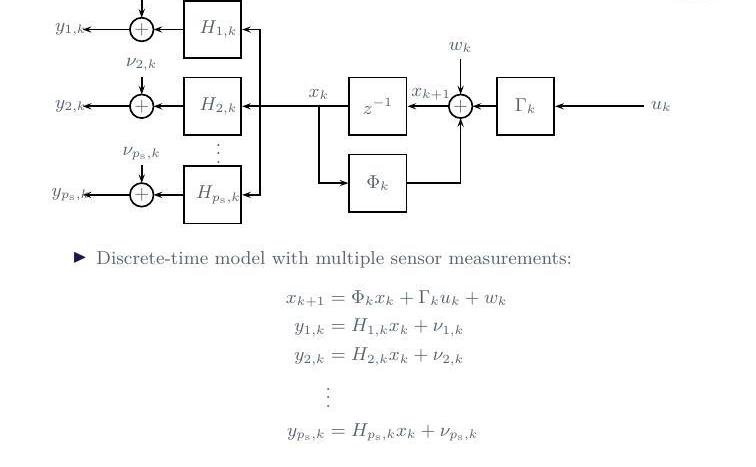
\includegraphics[width=\textwidth]{slide-07.jpg}
  \caption{Block diagram for a discrete-time system with $p_s$ sensors.
    The state $x_k$ evolves through the matrix $\Phi_k$ (the state transition)
    with input $u_k$ via gain $\Gamma_k$ and is driven by process noise $w_k$.
    Each of the $p_s$ sensors has its own observation matrix $H_{i,k}$ and
    adds its own measurement noise $\nu_{i,k}$ to produce output $y_{i,k}$.
    The $z^{-1}$ block is the unit delay: it holds the state for one time
    step, representing the discrete-time integration.
    The diagram makes clear that all sensors observe the \emph{same} state
    $x_k$ --- they differ only in which part of it they are sensitive to
    (which rows of $H_{i,k}$ are nonzero) and how noisy their channel is.}
\end{figure}

The system model is a straightforward extension of the single-sensor
discrete-time KF model.
The state evolves as before; the only change is that instead of one
measurement equation there are now $p_s$ of them --- one per sensor:

\[
  x_{k+1} = \Phi_k\, x_k + \Gamma_k\, u_k + w_k
\]
\[
  y_{1,k} = H_{1,k}\, x_k + \nu_{1,k}
\]
\[
  y_{2,k} = H_{2,k}\, x_k + \nu_{2,k}
\]
\[
  \vdots
\]
\[
  y_{p_s,k} = H_{p_s,k}\, x_k + \nu_{p_s,k}
\]

\begin{center}
\begin{tabular}{@{} l p{3.2cm} p{7.8cm} @{}}
  \toprule
  Symbol & Name & Meaning \\
  \midrule
  $x_k$ & State vector &
    The full physical state of the system at time step $k$
    (e.g.\ position, velocity, orientation). \\[3pt]
  $\Phi_k$ & State transition matrix &
    Propagates the state from step $k$ to step $k{+}1$ under the system
    dynamics.  If the dynamics are time-invariant, $\Phi_k = \Phi$ is
    constant. \\[3pt]
  $\Gamma_k$ & Input matrix &
    Maps the known control input $u_k$ into the state evolution. \\[3pt]
  $w_k$ & Process noise &
    Models unmodelled dynamics and disturbances.
    Assumed $\mathcal{N}(0, Q_k)$. \\[3pt]
  $p_s$ & Number of sensors &
    How many distinct sensors are fused.
    Each produces its own output $y_{i,k}$. \\[3pt]
  $y_{i,k}$ & Output of sensor $i$ &
    The raw measurement from sensor $i$ at time $k$.
    May have different physical units to $y_{j,k}$ for $j \neq i$. \\[3pt]
  $H_{i,k}$ & Observation matrix of sensor $i$ &
    Maps the state to what sensor $i$ actually measures.
    Different sensors can observe entirely different parts of the state. \\[3pt]
  $\nu_{i,k}$ & Measurement noise of sensor $i$ &
    The noise on sensor $i$'s reading.
    Its variance is $R_{ii,k}$; its correlation with sensor $j$ is
    $R_{ij,k}$. \\
  \bottomrule
\end{tabular}
\end{center}

\begin{notebox}
  \textbf{Why different $H_{i,k}$ matrices matter --- concrete examples}

  Suppose the full state vector is position and velocity in 3D:
  \[
    x_k =
    \begin{bmatrix} x \\ y \\ z \\ v_x \\ v_y \\ v_z \end{bmatrix}
    \leftarrow\text{position (metres)}
    \quad
    \leftarrow\text{velocity (m/s)}
  \]
  Three sensors are fused, each observing a different subset of this state.

  \bigskip
  \textbf{Sensor 1 --- GPS (measures full 3D position):}

  GPS gives you $(x, y, z)$ directly.
  It says nothing about velocity.
  So the measurement equation is:
  \[
    y_\text{GPS}
    = \begin{bmatrix} x \\ y \\ z \end{bmatrix}
    = \underbrace{\begin{bmatrix}
        1 & 0 & 0 & 0 & 0 & 0 \\
        0 & 1 & 0 & 0 & 0 & 0 \\
        0 & 0 & 1 & 0 & 0 & 0
      \end{bmatrix}}_{H_\text{GPS}}
    \begin{bmatrix} x \\ y \\ z \\ v_x \\ v_y \\ v_z \end{bmatrix}
    + \nu_\text{GPS}
  \]
  The first three columns of $H_\text{GPS}$ are an identity block because GPS
  reads position states directly --- a~1 in column~$i$ means ``pick out state
  component~$i$''.
  The last three columns are all zero because GPS tells us \emph{nothing}
  about velocity --- putting a~0 there instructs the filter not to try to
  infer velocity from this sensor's reading.

  \bigskip
  \textbf{Sensor 2 --- Barometer (measures altitude only):}

  A barometer measures only vertical position $z$ --- one number.
  It knows nothing about $x$, $y$, or any velocity component:
  \[
    y_\text{baro}
    = \begin{bmatrix} z \end{bmatrix}
    = \underbrace{\begin{bmatrix}
        0 & 0 & 1 & 0 & 0 & 0
      \end{bmatrix}}_{H_\text{baro}}
    \begin{bmatrix} x \\ y \\ z \\ v_x \\ v_y \\ v_z \end{bmatrix}
    + \nu_\text{baro}
  \]
  Column~3 is~1 (pick out $z$); every other column is~0
  (ignore everything else).
  The~0 in column~1 means: ``this sensor gives us no information about $x$,
  so do not let it influence the $x$ estimate.''
  The~0 in column~4 means: ``this sensor gives us no information about $v_x$,
  so do not let it influence the velocity estimate.''
  The filter will use the barometer \emph{only} to correct its $z$ estimate,
  leaving all other states unchanged by this particular measurement.

  \bigskip
  \textbf{Sensor 3 --- Doppler radar (measures radial velocity only):}

  A Doppler radar measures how fast the vehicle is approaching or receding
  --- that is, the velocity component along the beam direction.
  If the beam points along the $x$-axis, it measures $v_x$ only:
  \[
    y_\text{Doppler}
    = \begin{bmatrix} v_x \end{bmatrix}
    = \underbrace{\begin{bmatrix}
        0 & 0 & 0 & 1 & 0 & 0
      \end{bmatrix}}_{H_\text{Doppler}}
    \begin{bmatrix} x \\ y \\ z \\ v_x \\ v_y \\ v_z \end{bmatrix}
    + \nu_\text{Doppler}
  \]
  Now the~1 appears in column~4 (the $v_x$ component) and all position
  columns are~0.
  The Doppler radar directly constrains the velocity estimate without
  touching the position estimate at all.

  \bigskip
  \textbf{All three fused in one filter:}

  When all three sensors are active at the same step, the stacked
  measurement vector is:
  \[
    y_k =
    \begin{bmatrix} y_\text{GPS} \\ y_\text{baro} \\ y_\text{Doppler} \end{bmatrix}
    =
    \underbrace{\begin{bmatrix}
      1 & 0 & 0 & 0 & 0 & 0 \\
      0 & 1 & 0 & 0 & 0 & 0 \\
      0 & 0 & 1 & 0 & 0 & 0 \\
      0 & 0 & 1 & 0 & 0 & 0 \\
      0 & 0 & 0 & 1 & 0 & 0
    \end{bmatrix}}_{H_k}
    x_k + \nu_k
  \]
  Notice that the $z$ state appears in \emph{both} row~3 (GPS) and row~4
  (barometer) --- the filter automatically exploits both measurements to get
  a better $z$ estimate than either sensor could provide alone.
  The velocity state $v_x$ appears only in row~5 (Doppler), so only that
  sensor drives the velocity estimate.
  States $v_y$ and $v_z$ have no~1 in any row --- they are entirely
  unobserved by this sensor set and can only be tracked via the dynamic model.

  \textbf{What ``tracked via the dynamic model'' means --- the $\Phi_k$ matrix.}

  Yes, the dynamic model here is the state transition equation governed by
  $\Phi_k$.
  Even though no sensor ever directly reads $v_y$, the filter still maintains
  an estimate of it because $\Phi_k$ \emph{couples} $v_y$ to the position $y$,
  which GPS \emph{does} observe.

  In a constant-velocity model the state transition is:
  \[
    \begin{bmatrix} x \\ y \\ z \\ v_x \\ v_y \\ v_z \end{bmatrix}_{k+1}
    =
    \underbrace{\begin{bmatrix}
      1 & 0 & 0 & T_s & 0   & 0   \\
      0 & 1 & 0 & 0   & T_s & 0   \\
      0 & 0 & 1 & 0   & 0   & T_s \\
      0 & 0 & 0 & 1   & 0   & 0   \\
      0 & 0 & 0 & 0   & 1   & 0   \\
      0 & 0 & 0 & 0   & 0   & 1
    \end{bmatrix}}_{\Phi_k}
    \begin{bmatrix} x \\ y \\ z \\ v_x \\ v_y \\ v_z \end{bmatrix}_{k}
  \]
  Row~2 of $\Phi_k$ says $y_{k+1} = y_k + T_s v_{y,k}$.
  GPS measures $y$ at every step.
  So the filter sees that $y$ changed by some amount between steps, and because
  it knows $\Phi_k$ predicts $\Delta y = T_s v_y$, it can \emph{infer} what
  $v_y$ must have been --- even though $v_y$ was never directly measured.
  Over several GPS updates, the estimate of $v_y$ converges to the true value
  through this indirect coupling alone.

  In short: $H_k$ tells the filter what is \emph{directly} observed.
  $\Phi_k$ tells the filter how the unobserved states are \emph{linked} to
  the observed ones through the physics.
  Together they make it possible to estimate the full state even when no single
  sensor sees all of it.
\end{notebox}

% ------------------------------------------------------------------------------
\subsection*{2.2 \quad Assumptions --- The Correlated Noise Matrix $R_k$}
% ------------------------------------------------------------------------------

\begin{figure}[H]
  \centering
  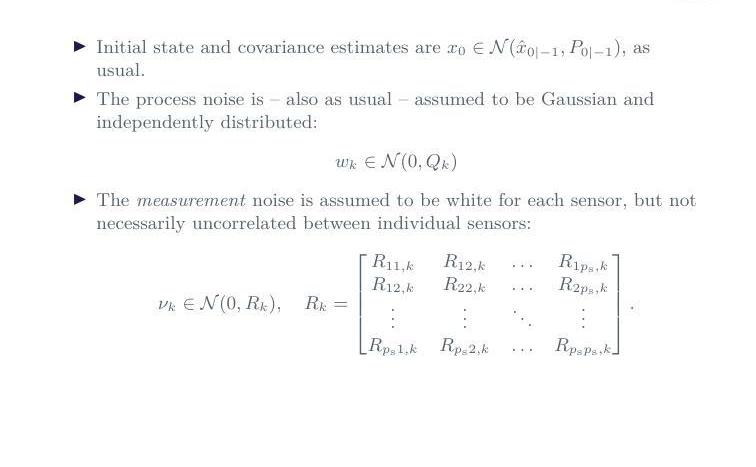
\includegraphics[width=\textwidth]{slide-08.jpg}
  \caption{Kalman filter assumptions for the multi-sensor case.
    The process noise assumption (Gaussian, independent) is identical to the
    single-sensor case.
    The new element is the \emph{measurement noise covariance matrix} $R_k$,
    which is now a $p_s \times p_s$ block matrix.
    The diagonal blocks $R_{ii,k}$ are the noise variances of the individual
    sensors; the off-diagonal blocks $R_{ij,k}$ ($i \neq j$) capture the
    \emph{correlations} between the noise of sensor $i$ and sensor $j$.}
\end{figure}

The standard KF assumptions carry over:

\begin{itemize}[leftmargin=1.4em, itemsep=3pt]
  \item The initial state is Gaussian:
    $x_0 \sim \mathcal{N}(\hat{x}_{0|-1},\, P_{0|-1})$.
  \item The process noise is Gaussian and independent across time steps:
    $w_k \sim \mathcal{N}(0,\, Q_k)$.
\end{itemize}

The one new assumption concerns the \textbf{joint measurement noise}.
Stack all $p_s$ sensor noise vectors into one:
\[
  \nu_k
  = \begin{bmatrix} \nu_{1,k} \\ \nu_{2,k} \\ \vdots \\ \nu_{p_s,k} \end{bmatrix}
  \sim \mathcal{N}(0,\, R_k),
  \qquad
  R_k =
  \begin{bmatrix}
    R_{11,k} & R_{12,k} & \cdots & R_{1p_s,k} \\
    R_{12,k} & R_{22,k} & \cdots & R_{2p_s,k} \\
    \vdots   & \vdots   & \ddots & \vdots      \\
    R_{p_s 1,k} & R_{p_s 2,k} & \cdots & R_{p_s p_s,k}
  \end{bmatrix}
\]

Each sensor's noise is assumed white (uncorrelated with its own past
values), but the noise of different sensors \emph{at the same time step}
may be correlated with each other.

\begin{notebox}
  \textbf{What each entry of $R_k$ means}

  Think of $R_k$ as a symmetric matrix that fully describes the noise
  behaviour of all sensors at time step $k$:

  \begin{itemize}[leftmargin=1.2em, itemsep=3pt]
    \item \textbf{Diagonal entry $R_{ii,k}$}: the \emph{variance} of the
      noise on sensor $i$ alone.
      Large $R_{ii,k}$ means sensor $i$ is noisy and should be trusted
      less by the filter.
      Small $R_{ii,k}$ means sensor $i$ is accurate and should be trusted
      more.
      This is exactly the $R$ from the single-sensor KF.

    \item \textbf{Off-diagonal entry $R_{ij,k}$ ($i \neq j$)}: the
      \emph{covariance} between the noise on sensor $i$ and the noise on
      sensor $j$ at the same time instant.
      If $R_{ij,k} > 0$, sensors $i$ and $j$ tend to make their errors in
      the same direction at the same time.
      If $R_{ij,k} = 0$, the two sensors' errors are independent of each
      other.
  \end{itemize}

  \textbf{When do off-diagonal terms arise in practice?}
  They appear when two sensors \emph{share a common noise source}:

  \begin{itemize}[leftmargin=1.2em, itemsep=2pt]
    \item Two accelerometers on the same rigid body both see the same
      vibration noise from the structure they are mounted on.
    \item Two GPS antennas at the same location receive the same
      atmospheric delay from the same satellites.
    \item Two temperature sensors in the same enclosure are both affected
      by the same thermal environment.
  \end{itemize}

  In all these cases, when one sensor's error spikes, the other's tends
  to spike in the same direction --- and the off-diagonal term captures
  exactly that tendency.
\end{notebox}

\begin{warnbox}
  \textbf{Why you cannot simply ignore the off-diagonal terms}

  If you incorrectly assume $R_k$ is diagonal when it is not
  (i.e.\ you set all $R_{ij} = 0$ for $i \neq j$), the Kalman filter
  still runs --- but it will produce a \emph{suboptimal} estimate.

  The filter weights each sensor independently, not knowing that sensors
  $i$ and $j$ are carrying redundant information.
  It may over-weight evidence that appears to come from two independent
  sources but is actually one shared error appearing twice.
  The estimated covariance $P_{k|k}$ will be too optimistic (too small),
  because the filter thinks it has more independent information than it
  actually does.

  Correctly accounting for $R_{ij}$ --- which is what the Cholesky
  decorrelation in Section~2.3 achieves --- ensures the filter is truly
  optimal.
\end{warnbox}

% ------------------------------------------------------------------------------
\subsection*{2.3 \quad Eliminating Correlations via Cholesky Factorisation}
% ------------------------------------------------------------------------------

\begin{figure}[H]
  \centering
  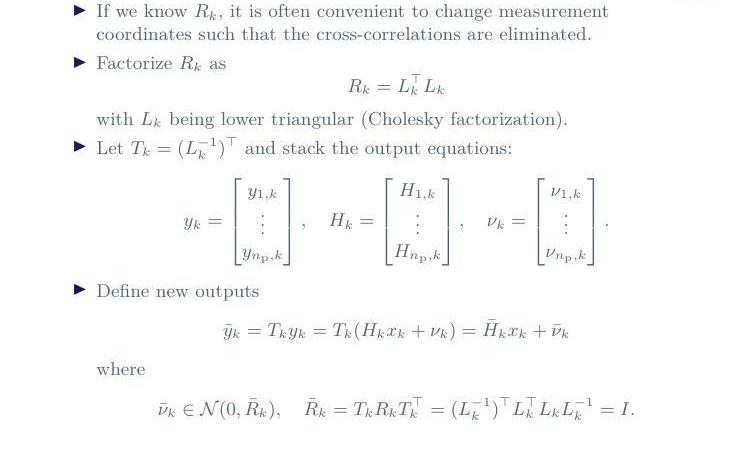
\includegraphics[width=\textwidth]{slide-09.jpg}
  \caption{The decorrelation procedure.
    \textbf{Top}: $R_k$ is factorised as $R_k = L_k^\top L_k$ (Cholesky).
    \textbf{Middle}: the stacked output vector $y_k$, stacked observation
    matrix $H_k$, and stacked noise vector $\nu_k$ are defined.
    \textbf{Bottom}: new transformed outputs $\bar{y}_k = T_k y_k$ are
    defined, where $T_k = (L_k^{-1})^\top$.
    The transformed noise $\bar{\nu}_k$ has covariance $\bar{R}_k = I$
    --- the sensors are now uncorrelated \emph{and} normalised to unit
    variance, making the standard KF update directly applicable.}
\end{figure}

The correlated $R_k$ prevents us from directly plugging the stacked
measurements into the standard Kalman filter, which assumes a diagonal
(or at least known, manageable) $R$.
The solution is to find a linear transformation $T_k$ that
\textbf{simultaneously decorrelates all sensor channels} and rescales them
to unit variance.
After the transformation, the standard KF update applies without any
modification.

\textbf{Step 1 --- Stack all sensor equations into one.}

Define the stacked vectors and matrices:
\[
  y_k = \begin{bmatrix} y_{1,k} \\ \vdots \\ y_{p_s,k} \end{bmatrix},
  \qquad
  H_k = \begin{bmatrix} H_{1,k} \\ \vdots \\ H_{p_s,k} \end{bmatrix},
  \qquad
  \nu_k = \begin{bmatrix} \nu_{1,k} \\ \vdots \\ \nu_{p_s,k} \end{bmatrix}
\]
so that all $p_s$ measurement equations collapse into one:
\[
  y_k = H_k\, x_k + \nu_k, \qquad \nu_k \sim \mathcal{N}(0,\, R_k)
\]
This is now formally identical to the single-sensor KF model, except that
$R_k$ is not diagonal.

\textbf{Step 2 --- Cholesky factorisation of $R_k$.}

Since $R_k$ is a covariance matrix it is symmetric positive definite.
Every such matrix has a unique \textbf{Cholesky factorisation}:
\[
  R_k = L_k^\top L_k
\]
where $L_k$ is a \textbf{lower triangular matrix} with positive diagonal
entries.

\begin{notebox}
  \textbf{What Cholesky factorisation is and why it works here}

  The Cholesky decomposition is the matrix analogue of taking the square root
  of a positive number.
  Just as any positive number $r$ can be written as $r = \sqrt{r} \cdot
  \sqrt{r}$, any symmetric positive definite matrix $R_k$ can be written as
  $R_k = L_k^\top L_k$, where $L_k$ plays the role of $\sqrt{R_k}$.

  The lower triangular structure of $L_k$ is not just a convenience ---
  it is what makes the factorisation unique and numerically efficient.
  A $p_s \times p_s$ matrix has $p_s^2$ entries, but a lower triangular one
  has only $p_s(p_s+1)/2$ entries.
  The Cholesky algorithm computes these entries in a single downward pass
  through the matrix, column by column.
  It is numerically stable and is the standard method used whenever a
  covariance matrix needs to be ``square-rooted''.

  \textbf{Why write $R_k = L_k^\top L_k$ and not $R_k = L_k L_k^\top$?}
  Both factorisations exist.
  The convention $R_k = L_k^\top L_k$ (with the transpose on the left)
  is chosen here because it makes $T_k = (L_k^{-1})^\top$ come out cleanly
  in Step~3.
  In MATLAB, \texttt{chol(R)} returns $L_k^\top$ by default (an upper
  triangular matrix), so the convention matches directly.
\end{notebox}

\textbf{Step 3 --- Define the decorrelating transformation $T_k$.}

Let:
\[
  T_k = (L_k^{-1})^\top
\]
This is the inverse of $L_k^\top$ --- equivalently, it is the transpose
of the inverse of $L_k$.
Now multiply both sides of the stacked measurement equation by $T_k$:
\[
  \underbrace{T_k y_k}_{\bar{y}_k}
  = T_k H_k\, x_k + T_k \nu_k
  = \underbrace{T_k H_k}_{\bar{H}_k}\, x_k
    + \underbrace{T_k \nu_k}_{\bar{\nu}_k}
\]
defining the \textbf{transformed output} $\bar{y}_k$,
\textbf{transformed observation matrix} $\bar{H}_k = T_k H_k$,
and \textbf{transformed noise} $\bar{\nu}_k = T_k \nu_k$.

\textbf{Step 4 --- Show that the transformed noise has identity covariance.}

Compute the covariance of $\bar{\nu}_k$:
\[
  \bar{R}_k
  = \mathrm{Cov}(\bar{\nu}_k)
  = T_k\, R_k\, T_k^\top
  = (L_k^{-1})^\top \cdot L_k^\top L_k \cdot \bigl((L_k^{-1})^\top\bigr)^\top
\]
Simplify the rightmost factor: $\bigl((L_k^{-1})^\top\bigr)^\top = L_k^{-1}$,
so:
\[
  \bar{R}_k
  = (L_k^{-1})^\top L_k^\top \cdot L_k L_k^{-1}
  = \bigl(L_k L_k^{-1}\bigr)^\top \cdot \bigl(L_k L_k^{-1}\bigr)
  = I^\top \cdot I
  = I
\]

The transformed noise has \textbf{identity covariance}: $\bar{\nu}_k \sim
\mathcal{N}(0, I)$.
Every channel is uncorrelated with every other and has unit variance.

\begin{notebox}
  \textbf{What the transformation actually does to the measurements ---
  intuition}

  Before the transformation, the $p_s$ sensor channels are
  \emph{entangled}: sensors $i$ and $j$ share part of the same error,
  so the two readings are not truly independent pieces of information.
  Using both naively would count the shared error twice.

  The matrix $T_k = (L_k^{-1})^\top$ \emph{untangles} them.
  Think of it as rotating and rescaling the measurement space so that the
  cross-sensor correlations disappear.
  After the transformation:
  \begin{itemize}[leftmargin=1.2em, itemsep=2pt]
    \item The channels of $\bar{y}_k$ are \emph{independent} (zero
      off-diagonal covariance in $\bar{R}_k = I$).
    \item Each channel has \emph{unit variance} (diagonal entries of
      $\bar{R}_k$ are all~1).
  \end{itemize}

  This means the transformed measurements $\bar{y}_k$ look exactly like
  independent, equally-weighted sensor readings --- which is exactly what
  the standard KF update assumes.
  No information has been lost or distorted: the transformation is
  invertible (multiply by $T_k^{-1}$ to recover the original), so it
  is a lossless change of coordinate system for the measurements.

  \textbf{Why normalising to unit variance matters:}
  After decorrelation, each transformed channel contributes equally to
  the Kalman gain computation.
  The filter's job then reduces to optimally weighting how informative
  each channel is about the state --- which it does via the updated
  $\bar{H}_k$ and the predicted state covariance $P_{k|k-1}$.
\end{notebox}

\begin{notebox}
  \textbf{Where does $R_k$ come from in practice?}

  $R_k$ is not computed by the filter --- you must supply it.
  It describes the noise statistics of your sensors and comes from two
  sources:

  \begin{itemize}[leftmargin=1.2em, itemsep=3pt]
    \item \textbf{Diagonal entries $R_{ii,k}$ --- individual sensor noise.}
      These are the easiest to get.
      Point each sensor at a known, fixed value and record a long sequence
      of readings.
      The sample variance of those readings gives you $R_{ii}$.
      Many sensor datasheets also quote a noise figure (e.g.\ ``RMS noise
      $= 0.05$\,m''), from which $R_{ii} = 0.05^2 = 0.0025$\,m$^2$.

    \item \textbf{Off-diagonal entries $R_{ij,k}$ --- cross-sensor
      correlations.}
      These are harder.
      You must run both sensors simultaneously, again pointed at a fixed
      known value, and compute the sample cross-covariance of their error
      sequences.
      If you have $N$ simultaneous readings:
      \[
        \hat{R}_{ij}
        = \frac{1}{N}\sum_{t=1}^{N}
          (y_{i,t} - \bar{y}_{i,t})(y_{j,t} - \bar{y}_{j,t})
      \]
      where $\bar{y}_{i,t}$ is the true value sensor $i$ should have read.
      If the sensors are physically separate and driven by different
      electronics, $R_{ij}$ is often zero or negligible and you can safely
      set it to zero.
      It becomes significant when two sensors share a power supply, a
      common clock, or are affected by the same environmental disturbance.
  \end{itemize}
\end{notebox}

\begin{notebox}
  \textbf{What do you actually apply $T_k$ to? --- A complete worked example}

  $T_k$ must be applied to \textbf{two things}: the observation matrix
  $H_k$ and the actual measurement $y_k$ at every step.
  Nothing else changes --- the state equations, $P_{k|k-1}$, and $Q_k$
  are all untouched.

  \medskip
  \textbf{Setup.}
  Two sensors both measure the same scalar state $x_k$
  (e.g.\ altitude), so both observation matrices are simply~1:
  \[
    H_{1,k} = H_{2,k} = 1
    \quad\Longrightarrow\quad
    H_k = \begin{bmatrix} 1 \\ 1 \end{bmatrix}
  \]
  Sensor~1 is noisier (variance 4), sensor~2 is more accurate (variance 2),
  and they share a common error source giving covariance~2:
  \[
    R_k = \begin{bmatrix} 4 & 2 \\ 2 & 2 \end{bmatrix}
  \]

  \textbf{Step 1 --- Cholesky factorisation} $R_k = L_k^\top L_k$.

  \textbf{Requirement for Cholesky to exist:} $R_k$ must be
  \textbf{symmetric positive definite} (SPD).
  Since $R_k$ is a covariance matrix of real sensor noise it is always
  symmetric, and positive definiteness is guaranteed as long as no sensor
  channel is a perfect deterministic function of another.
  If $R_k$ is only positive \emph{semi}definite (a degenerate case),
  Cholesky fails and the sensors must be reduced to a linearly independent
  subset first.

  Find lower-triangular $L_k$ such that $L_k^\top L_k = R_k$:
  \[
    L_k = \begin{bmatrix} 2 & 0 \\ 1 & 1 \end{bmatrix}
  \]
  Verify:
  \[
    L_k^\top L_k
    = \begin{bmatrix} 2 & 1 \\ 0 & 1 \end{bmatrix}
      \begin{bmatrix} 2 & 0 \\ 1 & 1 \end{bmatrix}
    = \begin{bmatrix} 4 & 2 \\ 2 & 2 \end{bmatrix}
    = R_k \checkmark
  \]

  \textbf{Step 2 --- Compute $T_k = (L_k^{-1})^\top$.}

  First invert $L_k$.
  For a $2\times2$ lower triangular matrix this is straightforward:
  \[
    L_k^{-1}
    = \begin{bmatrix} 1/2 & 0 \\ -1/2 & 1 \end{bmatrix}
  \]
  Verify: $L_k^{-1} L_k =
  \begin{bmatrix}1/2&0\\-1/2&1\end{bmatrix}
  \begin{bmatrix}2&0\\1&1\end{bmatrix}
  = \begin{bmatrix}1&0\\0&1\end{bmatrix} \checkmark$

  Now transpose:
  \[
    T_k = (L_k^{-1})^\top
        = \begin{bmatrix} 1/2 & -1/2 \\ 0 & 1 \end{bmatrix}
  \]

  \textbf{Step 3 --- Apply $T_k$ to $H_k$: get $\bar{H}_k$.}
  \[
    \bar{H}_k = T_k H_k
    = \begin{bmatrix} 1/2 & -1/2 \\ 0 & 1 \end{bmatrix}
      \begin{bmatrix} 1 \\ 1 \end{bmatrix}
    = \begin{bmatrix} 0 \\ 1 \end{bmatrix}
  \]
  Interesting: the first transformed channel has $\bar{H}_1 = 0$ ---
  it carries no information about $x_k$ at all after the transformation.
  The second transformed channel has $\bar{H}_2 = 1$ --- it is the only
  informative channel.

  \textbf{Why did sensor~1 become completely useless?}
  Yes --- in this example sensor~1 was essentially just a noisier,
  worse version of sensor~2.
  Think about what the two sensors gave us:
  \begin{itemize}[leftmargin=1.2em, itemsep=2pt]
    \item Sensor~2: reads the true state plus some noise $\nu_2$
      (variance~2).
    \item Sensor~1: reads the same true state plus the \emph{same} noise
      $\nu_2$ (the shared part, covariance~2) \emph{and} an extra
      independent noise term on top (bringing its total variance up
      to~4).
  \end{itemize}
  So sensor~1 = sensor~2's reading + extra garbage.
  Once you already have sensor~2, sensor~1 tells you nothing new ---
  everything it contains is either already in sensor~2 or is additional
  noise you do not want.
  The transformation discovers this automatically: the linear combination
  $\tfrac{1}{2}y_1 - \tfrac{1}{2}y_2$ (the first row of $T_k$) cancels
  out the true state entirely, leaving only noise.
  Naturally $\bar{H}_1 = 0$ --- the filter simply discards it.

  \textbf{This is not always what happens.}
  It is a consequence of the correlation being very strong here
  ($R_{12} = 2$ out of a theoretical maximum of
  $\sqrt{R_{11} \cdot R_{22}} = \sqrt{4 \cdot 2} \approx 2.83$,
  so about 71\% of the maximum possible correlation).
  With weaker correlation both transformed channels would still have
  nonzero $\bar{H}$ values and both would contribute to the update,
  just with appropriately adjusted weights.
  The transformation does not decide to throw sensors away --- it simply
  exposes the truth about how much independent information each sensor
  actually carries, and in this case sensor~1 carried none.

  \textbf{Step 4 --- Apply $T_k$ to the actual measurement $y_k$: get
  $\bar{y}_k$.}

  Suppose at this time step sensor~1 reads $y_{1,k} = 10.3$\,m and
  sensor~2 reads $y_{2,k} = 9.8$\,m:
  \[
    \bar{y}_k = T_k y_k
    = \begin{bmatrix} 1/2 & -1/2 \\ 0 & 1 \end{bmatrix}
      \begin{bmatrix} 10.3 \\ 9.8 \end{bmatrix}
    = \begin{bmatrix} 0.25 \\ 9.8 \end{bmatrix}
  \]
  The first transformed reading is $0.25$ but its $\bar{H}_1 = 0$, so it
  contributes nothing to the state update --- the filter ignores it.
  The second transformed reading $9.8$ has $\bar{H}_2 = 1$ and this is
  what the filter uses to update its altitude estimate.

  \textbf{Step 5 --- Verify $\bar{R}_k = I$.}
  \[
    \bar{R}_k = T_k R_k T_k^\top
    = \begin{bmatrix} 1/2 & -1/2 \\ 0 & 1 \end{bmatrix}
      \begin{bmatrix} 4 & 2 \\ 2 & 2 \end{bmatrix}
      \begin{bmatrix} 1/2 & 0 \\ -1/2 & 1 \end{bmatrix}
    = \begin{bmatrix} 1 & 0 \\ 0 & 1 \end{bmatrix}
    = I \checkmark
  \]
  The two transformed channels now have unit variance and zero
  cross-correlation --- their noise is completely independent.
  The standard KF update can be applied directly using $\bar{H}_k$ and
  $\bar{R}_k = I$.

  \textbf{Summary of what $T_k$ is applied to:}
  \begin{center}
  \begin{tabular}{@{} l l l @{}}
    \toprule
    Quantity & Before transformation & After transformation \\
    \midrule
    Observation matrix & $H_k$ & $\bar{H}_k = T_k H_k$ \\
    Actual measurement & $y_k$ & $\bar{y}_k = T_k y_k$ \\
    Noise covariance   & $R_k$ (correlated) & $\bar{R}_k = I$ (independent) \\
    State / covariance & $x_k,\; P_{k|k-1}$ & unchanged \\
    \bottomrule
  \end{tabular}
  \end{center}
\end{notebox}

% ------------------------------------------------------------------------------
\subsection*{2.4 \quad The Full KF Update with Transformed Measurements}
% ------------------------------------------------------------------------------

\begin{figure}[H]
  \centering
  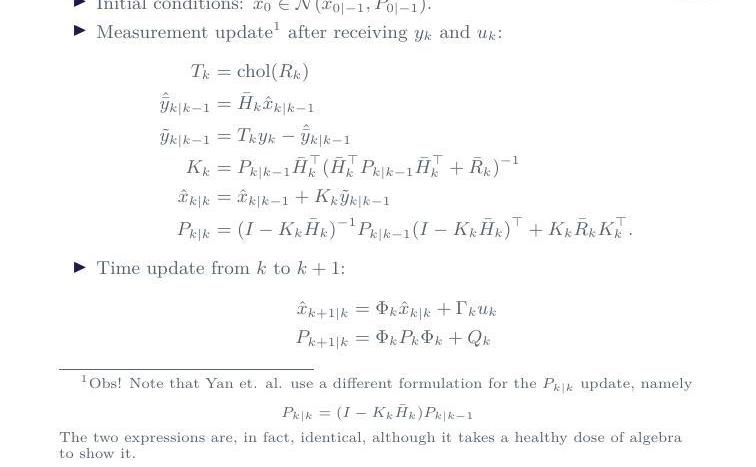
\includegraphics[width=\textwidth]{slide-10.jpg}
  \caption{Complete Kalman filter equations for multi-sensor fusion using the
    transformed measurements.
    The footnote on the slide notes that an alternative (Joseph) form of the
    $P_{k|k}$ update is used here, which is numerically more stable than the
    simple $(I - K_k \bar{H}_k) P_{k|k-1}$ form; the two are algebraically
    identical.}
\end{figure}

Once the transformation $T_k$ has been computed and applied, the Kalman
filter runs in exactly the same form as the single-sensor case, but on the
transformed quantities $(\bar{y}_k, \bar{H}_k, \bar{R}_k = I)$.

\textbf{Initialisation:}
\[
  x_0 \sim \mathcal{N}(\hat{x}_{0|-1},\; P_{0|-1})
\]

\textbf{Measurement update} (after receiving $y_k$ and $u_k$ at step $k$):

First compute the transformation:
\[
  T_k = \mathrm{chol}(R_k)
\]

\begin{notebox}
  \textbf{What \texttt{chol} returns --- matching the convention}

  In MATLAB, \texttt{chol(R)} returns the upper triangular factor $U$
  such that $R = U^\top U$.
  Comparing with our convention $R_k = L_k^\top L_k$, we have
  $U = L_k$ and so \texttt{chol(R)} gives $L_k$ directly.
  Therefore $T_k = (L_k^{-1})^\top = (\texttt{chol(R)}^{-1})^\top$.
  In the slide the notation $T_k = \mathrm{chol}(R_k)$ is shorthand for
  this full computation.
\end{notebox}

Predicted (transformed) output:
\[
  \hat{y}_{k|k-1} = \bar{H}_k\, \hat{x}_{k|k-1}
\]

Transformed innovation (the ``surprise'' from the new measurements):
\[
  \tilde{y}_{k|k-1} = T_k y_k - \hat{y}_{k|k-1}
\]

Kalman gain:
\[
  K_k = P_{k|k-1}\, \bar{H}_k^\top
        \bigl(\bar{H}_k P_{k|k-1} \bar{H}_k^\top + \bar{R}_k\bigr)^{-1}
\]

State estimate update:
\[
  \hat{x}_{k|k} = \hat{x}_{k|k-1} + K_k\, \tilde{y}_{k|k-1}
\]

Covariance update (Joseph/symmetric form):
\[
  P_{k|k} = (I - K_k \bar{H}_k)\, P_{k|k-1}\, (I - K_k \bar{H}_k)^\top
            + K_k \bar{R}_k K_k^\top
\]

\textbf{Time update} (propagation from step $k$ to $k{+}1$):
\[
  \hat{x}_{k+1|k} = \Phi_k\, \hat{x}_{k|k} + \Gamma_k\, u_k
\]
\[
  P_{k+1|k} = \Phi_k\, P_{k|k}\, \Phi_k^\top + Q_k
\]

\begin{center}
\begin{tabular}{@{} l p{3.5cm} p{7.0cm} @{}}
  \toprule
  Symbol & Name & Meaning \\
  \midrule
  $T_k$ & Decorrelating transform &
    $T_k = (L_k^{-1})^\top$ where $L_k$ comes from Cholesky of $R_k$.
    Applied once per step before everything else. \\[3pt]
  $\bar{H}_k$ & Transformed observation matrix &
    $\bar{H}_k = T_k H_k$.
    Used in place of $H_k$ throughout the update step. \\[3pt]
  $\bar{R}_k$ & Transformed noise covariance &
    $\bar{R}_k = I$ always, by construction of $T_k$.
    The standard KF sees perfectly decorrelated unit-variance channels. \\[3pt]
  $\hat{x}_{k|k-1}$ & Predicted state &
    Best estimate of $x_k$ before the new measurements are used,
    carried over from the previous time update. \\[3pt]
  $\tilde{y}_{k|k-1}$ & Innovation &
    The gap between what was measured ($T_k y_k$, i.e.\ the transformed
    actual reading) and what was predicted ($\hat{y}_{k|k-1}$).
    A large innovation means the model was surprised ---
    either the measurement is informative, or the model is wrong. \\[3pt]
  $K_k$ & Kalman gain &
    Weights how much the innovation corrects the state estimate.
    Larger $K_k$ means more trust in the measurements;
    smaller means more trust in the model. \\[3pt]
  $P_{k|k}$ & Updated state covariance &
    How uncertain the state estimate is after incorporating the
    measurements.  Should be smaller than $P_{k|k-1}$. \\[3pt]
  $P_{k+1|k}$ & Predicted state covariance &
    Propagated uncertainty before the next measurement update.
    Grows due to process noise $Q_k$. \\
  \bottomrule
\end{tabular}
\end{center}

\begin{notebox}
  \textbf{Why the Joseph form of the covariance update is used}

  The standard simplified covariance update is:
  \[
    P_{k|k} = (I - K_k \bar{H}_k)\, P_{k|k-1}
  \]
  This is algebraically correct \emph{only when} $K_k$ is exactly the
  optimal Kalman gain.
  In finite-precision computer arithmetic, rounding errors accumulate
  and $K_k$ is never computed perfectly.
  Even small errors in $K_k$ can cause the simplified formula to produce
  a $P_{k|k}$ that is slightly non-symmetric or even not positive
  semi-definite --- which would cause the filter to diverge or produce
  nonsensical negative variances.

  The \textbf{Joseph (symmetric) form}:
  \[
    P_{k|k} = (I - K_k \bar{H}_k)\, P_{k|k-1}\, (I - K_k \bar{H}_k)^\top
              + K_k \bar{R}_k K_k^\top
  \]
  is \emph{always} symmetric and positive semi-definite by construction,
  even with non-optimal $K_k$ and finite-precision arithmetic.
  The extra $K_k \bar{R}_k K_k^\top$ term adds back the measurement noise
  contribution that is lost when $K_k$ is not exactly optimal, ensuring
  the covariance is never underestimated.
  This is the numerically safe form and should always be preferred in
  implementation.
\end{notebox}

\begin{notebox}
  \textbf{The full algorithm at a glance --- what runs each step}

  At every time step $k$ the filter does the following, in order:

  \begin{enumerate}[leftmargin=1.6em, itemsep=4pt]
    \item \textbf{Receive} the new measurement vector $y_k$ (all sensors
      stacked) and the known input $u_k$.

    \item \textbf{Compute} $T_k = \mathrm{chol}(R_k)$ and
      $\bar{H}_k = T_k H_k$.
      If $R_k$ is constant over time this is done once offline.

    \item \textbf{Form the innovation:}
      $\tilde{y}_{k|k-1} = T_k y_k - \bar{H}_k \hat{x}_{k|k-1}$.

    \item \textbf{Compute the Kalman gain:}
      $K_k = P_{k|k-1} \bar{H}_k^\top
      (\bar{H}_k P_{k|k-1} \bar{H}_k^\top + I)^{-1}$.
      Note: $\bar{R}_k = I$ so no $R$ appears in the gain formula.

    \item \textbf{Update state and covariance:}
      $\hat{x}_{k|k}$ and $P_{k|k}$ via the formulas above.

    \item \textbf{Time update:} propagate
      $\hat{x}_{k+1|k} = \Phi_k \hat{x}_{k|k} + \Gamma_k u_k$
      and
      $P_{k+1|k} = \Phi_k P_{k|k} \Phi_k^\top + Q_k$.
  \end{enumerate}

  Steps~2--5 are the \emph{measurement update}; step~6 is the
  \emph{time update}.
  The two-step structure is identical to the single-sensor KF ---
  the Cholesky transformation in step~2 is the only addition.
  If $R_k$ is constant (time-invariant sensor noise), $T_k$ and
  $\bar{H}_k$ are precomputed once and the runtime cost is exactly the
  same as a standard KF.
\end{notebox}

\begin{warnbox}
  \textbf{Units --- the most common practical mistake in multi-sensor fusion}

  The slide states that different sensors can give measurements ``in vastly
  different units.''
  This is not just a cosmetic issue --- it directly affects the filter.

  Suppose sensor~1 measures position in metres ($y_1 \sim 1$--$100$\,m)
  and sensor~2 measures it in millimetres ($y_2 \sim 1000$--$100{,}000$\,mm).
  The raw numerical values differ by a factor of 1000.
  If you stack them directly without converting to common units, the $R_k$
  matrix will have entries that differ by $10^6$ (the square of 1000),
  and the Kalman gain will be wildly skewed toward the sensor with the
  numerically larger readings --- which is the less precise one in physical
  terms.

  \textbf{Rule}: always convert all sensor outputs to a consistent set of
  units (e.g.\ SI: metres, radians, seconds) before stacking them into $y_k$
  and forming $R_k$.
  The Cholesky decorrelation does not fix unit mismatches --- it only removes
  statistical correlations between correctly-scaled channels.
\end{warnbox}

% ── Key takeaways ─────────────────────────────────────────────────────────────
\begin{keybox}
  \textbf{Section 2 --- Key Takeaways}
  \begin{itemize}[leftmargin=1.2em, itemsep=2pt]
    \item The multi-sensor model has one state equation and $p_s$
      measurement equations, one per sensor:
      $y_{i,k} = H_{i,k} x_k + \nu_{i,k}$.
      Different $H_{i,k}$ matrices allow sensors measuring completely
      different physical quantities to be fused inside one filter.

    \item The joint noise covariance $R_k$ is a $p_s \times p_s$ matrix.
      \textbf{Diagonal entries} $R_{ii,k}$ are individual sensor variances;
      \textbf{off-diagonal entries} $R_{ij,k}$ capture noise correlations
      between sensors sharing a common error source.
      Ignoring off-diagonal terms gives a suboptimal, overconfident filter.

    \item \textbf{Cholesky decorrelation}: factorise $R_k = L_k^\top L_k$,
      set $T_k = (L_k^{-1})^\top$, and transform:
      $\bar{y}_k = T_k y_k$,\; $\bar{H}_k = T_k H_k$,\;
      $\bar{R}_k = T_k R_k T_k^\top = I$.
      The transformed channels are independent and unit-variance.

    \item After the transformation the \textbf{standard KF update} applies
      unchanged, with $\bar{H}_k$ and $\bar{R}_k = I$ in place of $H_k$
      and $R_k$.
      Use the \textbf{Joseph form} of the covariance update to maintain
      positive definiteness under finite-precision arithmetic.

    \item Always convert all sensor readings to \textbf{consistent units}
      before stacking --- unit mismatches corrupt $R_k$ and bias the
      Kalman gain.
  \end{itemize}
\end{keybox}

% ==============================================================================
\newpage
\section*{Section 3 \quad Complementary Filter}
% ==============================================================================

The Kalman filter from Section~2 is the optimal solution for multi-sensor
fusion when you have a state-space model, Gaussian noise, and known noise
covariances.
But sometimes the situation is simpler: you have \emph{two sensors that
measure related quantities} --- one good at low frequencies, one good at high
frequencies --- and you want a clean estimate of the underlying signal without
building a full state-space model.
The \textbf{complementary filter} is the tool for this.
It is simple, computationally cheap, and widely used in embedded systems such
as drones and robots where the full KF overhead is not justified.

% ------------------------------------------------------------------------------
\subsection*{3.1 \quad Core Idea --- Splitting the Frequency Spectrum}
% ------------------------------------------------------------------------------

\begin{figure}[H]
  \centering
  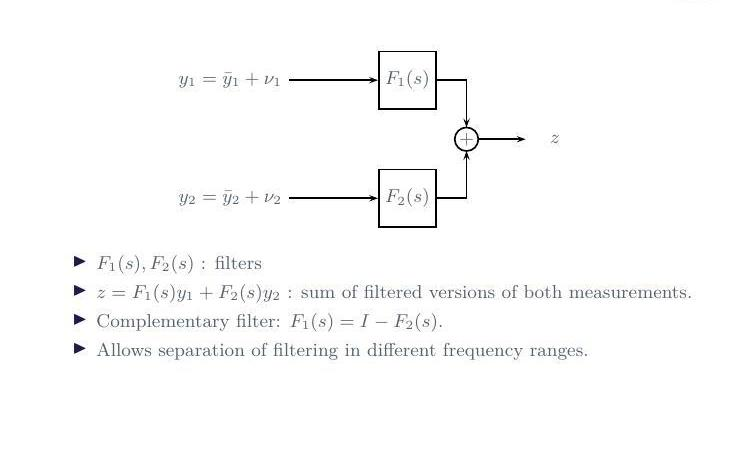
\includegraphics[width=\textwidth]{slide-11.jpg}
  \caption{General complementary filter architecture.
    Two sensors produce noisy measurements $y_1$ and $y_2$ of related
    quantities.
    Each passes through its own filter $F_1(s)$ and $F_2(s)$.
    The outputs are summed to give the final estimate $z$.
    The complementary condition $F_1(s) = I - F_2(s)$ ensures the two
    filters together cover the full frequency spectrum without overlap or
    gap --- whatever $F_2$ does not pass, $F_1$ picks up, and vice versa.}
\end{figure}

The general structure is:
\[
  z = F_1(s)\, y_1 + F_2(s)\, y_2
\]
where $y_1$ and $y_2$ are two measurements, $F_1(s)$ and $F_2(s)$ are
linear filters (transfer functions in the Laplace domain), and $z$ is the
fused estimate of the quantity of interest.

The defining property of a complementary filter is:
\[
  \boxed{F_1(s) = I - F_2(s)}
  \quad\Longleftrightarrow\quad
  F_1(s) + F_2(s) = I
\]

\begin{notebox}
  \textbf{What $F_1(s) + F_2(s) = I$ means and why it is called
  ``complementary''}

  Think of $F_2(s)$ as a \textbf{low-pass filter} --- it passes slow,
  low-frequency content and blocks fast variations.
  Then $F_1(s) = I - F_2(s)$ is its \textbf{high-pass complement} ---
  it passes exactly what the low-pass blocks and blocks what the low-pass
  passes.

  Together, at every frequency:
  \begin{itemize}[leftmargin=1.2em, itemsep=2pt]
    \item At \textbf{low frequencies}: $F_2 \approx 1$, so $F_1 \approx 0$.
      The output $z \approx y_2$ --- the estimate is dominated by sensor~2.
    \item At \textbf{high frequencies}: $F_2 \approx 0$, so $F_1 \approx 1$.
      The output $z \approx y_1$ --- the estimate is dominated by sensor~1.
    \item At \textbf{all frequencies combined}: $F_1 + F_2 = 1$, so no
      frequency is either double-counted or missing from the output.
  \end{itemize}

  This is where the name comes from: $F_1$ and $F_2$ are
  \emph{complementary} in the literal sense --- each covers the frequency
  range the other does not.
  The design question reduces to: choose $F_2$ (the low-pass), and $F_1$
  is determined automatically.

  \textbf{What if both sensors capture some of the same frequency range?}

  If the two sensors overlap --- both are reliable in some shared band ---
  the complementary filter still runs without breaking, but it becomes
  \textbf{suboptimal} and you lose the main benefit.

  Here is what happens in the overlap region.
  Because $F_1 + F_2 = 1$, the filter assigns every frequency either mostly
  to sensor~1 or mostly to sensor~2, depending on which side of the crossover
  $1/\tau$ that frequency sits.
  In the overlap band, where \emph{both} sensors are reliable, the filter
  still only uses one of them at a time --- it never combines both.
  You are therefore throwing away valid information from whichever sensor
  the filter is downweighting at that frequency.

  A \textbf{Kalman filter} handles this correctly: it has a separate noise
  variance for each sensor and computes the optimal weighted average at every
  frequency, automatically giving more weight to the better sensor at each
  frequency and using both when they are equally reliable.
  The complementary filter cannot do this because it has only one tuning
  parameter ($\tau$) to describe all trade-offs.

  \textbf{The extreme case --- two sensors measuring exactly the same thing:}
  If both sensors observe the same quantity at all frequencies (e.g.\ two GPS
  receivers of the same type), the complementary filter reduces to: use
  sensor~2 at low frequencies and sensor~1 at high frequencies.
  You are still only ever using one sensor at a time and completely ignoring
  the other's reading in its assigned band, even though both are equally
  valid.
  The right tool here is a KF (or simply averaging the two readings with
  inverse-variance weights), not a complementary filter.

  \textbf{Rule of thumb:} use a complementary filter when your sensors have
  clearly \emph{non-overlapping} strength regions --- one is good where the
  other is bad. When there is significant overlap, switch to a Kalman filter.

  \textbf{Why split by frequency?}
  Different sensors tend to be reliable in different frequency ranges:
  \begin{itemize}[leftmargin=1.2em, itemsep=2pt]
    \item A \textbf{gyroscope} integrates cleanly at high frequencies (fast
      rotations) but drifts at low frequencies (slow bias builds up over
      time).
    \item An \textbf{accelerometer or magnetometer} gives a stable
      low-frequency reference (gravity direction, magnetic north) but is
      corrupted by vibration at high frequencies.
  \end{itemize}
  Assigning the high-frequency band to the gyroscope and the low-frequency
  band to the accelerometer --- and summing them with complementary filters
  --- exploits the strength of each sensor while rejecting its weakness.
  This exact idea is at the heart of the Madgwick and Mahoney filters
  developed in Sections~6 and~7.
\end{notebox}

% ------------------------------------------------------------------------------
\subsection*{3.2 \quad Continuous-Time Example: Position from Velocity and
Position}
% ------------------------------------------------------------------------------

\begin{figure}[H]
  \centering
  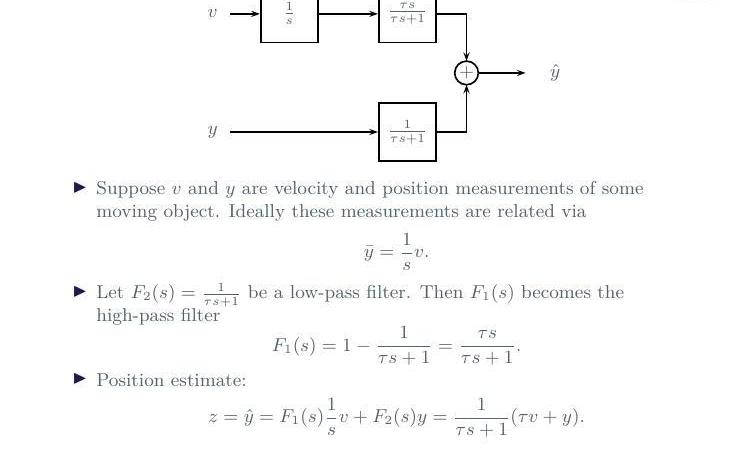
\includegraphics[width=\textwidth]{slide-12.jpg}
  \caption{Complementary filter for fusing a \textbf{velocity} measurement
    $v$ and a \textbf{position} measurement $y$.
    The velocity is first integrated ($1/s$) to produce a position estimate,
    then passed through the high-pass filter $F_1(s) = \tfrac{\tau s}{\tau s+1}$.
    The position measurement passes through the low-pass filter
    $F_2(s) = \tfrac{1}{\tau s+1}$.
    Both are summed to give the fused position estimate $\hat{y}$.
    The time constant $\tau$ controls where the crossover between the two
    sensors occurs.}
\end{figure}

Suppose you have two sensors on a moving object:
\begin{itemize}[leftmargin=1.4em, itemsep=2pt]
  \item \textbf{Sensor 1}: measures \emph{velocity} $v$ (e.g.\ a tachometer
    or Doppler radar). Fast and accurate at high frequencies but cannot give
    you absolute position --- you must integrate to get there.
  \item \textbf{Sensor 2}: measures \emph{position} $y$ directly
    (e.g.\ GPS). Gives absolute position but is slow and noisy at high
    frequencies.
\end{itemize}

If the sensor measurements were perfect, position and velocity would be
related by:
\[
  \bar{y} = \frac{1}{s}\, v
\]
where $1/s$ denotes integration in the Laplace domain
($\bar{y}$ is the ideal noise-free position, $v$ is the noise-free velocity).
In reality both measurements are noisy, and direct integration of a noisy
velocity drifts without bound.

\textbf{Choosing the filters.}

Let $F_2(s)$ be a first-order low-pass filter with time constant $\tau$:
\[
  F_2(s) = \frac{1}{\tau s + 1}
\]
By the complementary condition, $F_1(s)$ is automatically:
\[
  F_1(s)
  = I - F_2(s)
  = 1 - \frac{1}{\tau s + 1}
  = \frac{\tau s + 1 - 1}{\tau s + 1}
  = \frac{\tau s}{\tau s + 1}
\]
This is a first-order \textbf{high-pass filter} with the same time constant
$\tau$.

\textbf{The fused position estimate.}

Sensor~1 contributes via integration then high-pass filtering;
sensor~2 contributes via direct low-pass filtering.
The output is:
\[
  z = \hat{y}
    = F_1(s)\cdot\frac{1}{s}\cdot v + F_2(s)\cdot y
    = \frac{\tau s}{\tau s+1}\cdot\frac{v}{s}
      + \frac{1}{\tau s+1}\cdot y
    = \frac{\tau v}{\tau s+1} + \frac{y}{\tau s+1}
    = \frac{1}{\tau s+1}\bigl(\tau v + y\bigr)
\]

So the complete estimate is:
\[
  \boxed{\hat{y} = \frac{1}{\tau s + 1}\,(\tau\, v + y)}
\]

\begin{center}
\begin{tabular}{@{} l p{3.0cm} p{7.5cm} @{}}
  \toprule
  Symbol & Name & Meaning \\
  \midrule
  $v$ & Velocity measurement &
    Raw reading from sensor~1 (e.g.\ tachometer, Doppler).
    Good at high frequencies; integrates to position but drifts. \\[3pt]
  $y$ & Position measurement &
    Raw reading from sensor~2 (e.g.\ GPS).
    Good at low frequencies; gives absolute position but noisy at high
    frequencies. \\[3pt]
  $\hat{y}$ & Fused position estimate &
    The complementary filter output --- a weighted combination of both
    sensors that takes the best from each. \\[3pt]
  $\tau$ & Time constant &
    Sets the crossover frequency $\omega_c = 1/\tau$ between the two
    sensors.
    Below $\omega_c$: GPS dominates.
    Above $\omega_c$: velocity integration dominates. \\[3pt]
  $F_1(s) = \tfrac{\tau s}{\tau s+1}$ & High-pass filter &
    Applied to the integrated velocity.
    Passes fast position changes well; removes the low-frequency drift
    from integration. \\[3pt]
  $F_2(s) = \tfrac{1}{\tau s+1}$ & Low-pass filter &
    Applied to the GPS position.
    Passes the slow, absolute position reference; removes high-frequency
    GPS noise. \\
  \bottomrule
\end{tabular}
\end{center}

\begin{notebox}
  \textbf{Intuition for the formula $\hat{y} = \frac{1}{\tau s+1}(\tau v + y)$}

  Rewrite slightly by multiplying out:
  \[
    (\tau s + 1)\hat{y} = \tau v + y
  \]
  In the time domain this is a first-order differential equation:
  \[
    \tau\,\dot{\hat{y}} + \hat{y} = \tau\, v + y
  \]
  This is saying: the estimate $\hat{y}$ is driven by two terms:
  \begin{itemize}[leftmargin=1.2em, itemsep=3pt]
    \item $\tau v$: the velocity measurement scaled by $\tau$ --- this term
      drives $\hat{y}$ to change at the measured rate $v$.
      Since $\tau v$ is proportional to velocity, it acts like integration
      of $v$ (it adds the velocity contribution to the estimate).
    \item $y$: the GPS position --- this term continuously pulls $\hat{y}$
      back toward the absolute GPS reading, preventing drift.
  \end{itemize}
  The time constant $\tau$ controls the relative weight: large $\tau$
  trusts velocity more (faster dynamics, more responsive to $v$); small
  $\tau$ trusts GPS more (estimate stays close to $y$).

  \textbf{What happens at the extremes of $\tau$:}
  \begin{itemize}[leftmargin=1.2em, itemsep=2pt]
    \item $\tau \to 0$: $F_1 \to 0$, $F_2 \to 1$, $\hat{y} \to y$.
      The filter ignores the velocity entirely and just outputs the GPS
      reading directly.
    \item $\tau \to \infty$: $F_2 \to 0$, $F_1 \to 1$, $\hat{y} \to
      \tfrac{1}{s}v$ (pure velocity integration).
      The GPS is completely ignored and the estimate drifts freely.
    \item A finite $\tau$: the GPS prevents long-term drift while the
      velocity integration gives smooth, high-rate position updates between
      slow GPS fixes.
  \end{itemize}
\end{notebox}

\begin{notebox}
  \textbf{How does this relate to the Kalman filter?}

  The complementary filter and the Kalman filter for the same problem
  (fusing position and velocity) produce \emph{identical results} when the
  Kalman filter has converged and the noise statistics happen to match the
  implied weighting of the complementary filter.

  The key difference is how $\tau$ is chosen:
  \begin{itemize}[leftmargin=1.2em, itemsep=2pt]
    \item In the \textbf{complementary filter}, $\tau$ is a design parameter
      you set by engineering judgement --- typically based on knowing roughly
      how noisy GPS is versus the velocity sensor.
    \item In the \textbf{Kalman filter}, the equivalent of $\tau$ emerges
      automatically from the noise covariances $Q$ and $R$ that you supply.
      The filter computes the optimal crossover frequency for you.
  \end{itemize}
  The complementary filter is therefore a computationally cheap, tuning-by-
  hand version of the Kalman filter for problems where the sensors split
  cleanly into ``good at high frequencies'' and ``good at low frequencies''.
  When this split is clean, the complementary filter is often preferred in
  embedded systems for its simplicity and low CPU cost.
\end{notebox}

% ------------------------------------------------------------------------------
\subsection*{3.3 \quad Discrete-Time Implementation}
% ------------------------------------------------------------------------------

\begin{figure}[H]
  \centering
  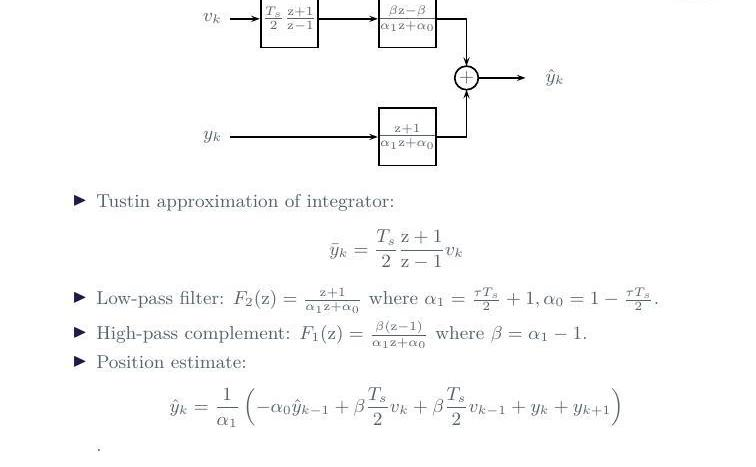
\includegraphics[width=\textwidth]{slide-13.jpg}
  \caption{Discrete-time complementary filter block diagram.
    The integrator $1/s$ is approximated by the Tustin (bilinear) method,
    giving the discrete-time factor $\tfrac{T_s}{2}\tfrac{z+1}{z-1}$.
    The low-pass filter $F_2$ and its high-pass complement $F_1$ are also
    expressed in the $z$-domain.
    All three blocks operate on sampled signals with sample period $T_s$,
    and their outputs are summed to give the discrete-time position estimate
    $\hat{y}_k$.}
\end{figure}

To implement the complementary filter on a digital processor, every
continuous-time block must be converted to a discrete-time equivalent.
The standard method is the \textbf{Tustin (bilinear) approximation}, which
replaces the Laplace variable $s$ with:
\[
  s \;\longleftarrow\; \frac{2}{T_s}\cdot\frac{z - 1}{z + 1}
\]
where $T_s$ is the sample period and $z$ is the $z$-transform variable
(one step forward in time).

\begin{notebox}
  \textbf{Why Tustin}
  \begin{itemize}
    \item \textbf{Tustin / bilinear} ($s \leftarrow \frac{2}{T_s}
      \frac{z-1}{z+1}$): maps the left half of the $s$-plane
      \emph{exactly} onto the interior of the unit disc, preserving
      stability.
      It also preserves the frequency response shape much more accurately
      than the Euler methods up to the Nyquist frequency.
  \end{itemize}
  For a complementary filter where precise frequency-domain behaviour
  matters (the crossover frequency $1/\tau$ must be where you designed it),
  Tustin is the right choice.
\end{notebox}

\textbf{Tustin approximation of the integrator $1/s$:}
\[
  \frac{1}{s}
  \;\longrightarrow\;
  \frac{T_s}{2}\cdot\frac{z + 1}{z - 1}
\]
Applied to the velocity $v_k$, this gives the approximate integrated position:
\[
  \bar{y}_k = \frac{T_s}{2}\cdot\frac{z+1}{z-1}\, v_k
\]
In the time domain: $\bar{y}_k = \bar{y}_{k-1} + \tfrac{T_s}{2}(v_k + v_{k-1})$
--- this is simply the \textbf{trapezoidal integration rule}: the area under
the velocity curve between steps $k{-}1$ and $k$ is approximated as the
average of the two endpoint velocities times the step width $T_s$.

\textbf{Discrete-time low-pass filter $F_2$:}

Applying the Tustin substitution to $F_2(s) = \tfrac{1}{\tau s + 1}$:
\[
  F_2(z) = \frac{z + 1}{\alpha_1 z + \alpha_0}
\]
where the coefficients are:
\[
  \alpha_1 = \frac{\tau T_s}{2} + 1, \qquad \alpha_0 = 1 - \frac{\tau T_s}{2}
\]

\textbf{Discrete-time high-pass complement $F_1$:}

Since $F_1(z) = 1 - F_2(z)$:
\[
  F_1(z)
  = 1 - \frac{z+1}{\alpha_1 z + \alpha_0}
  = \frac{(\alpha_1 z + \alpha_0) - (z+1)}{\alpha_1 z + \alpha_0}
  = \frac{(\alpha_1 - 1)z + (\alpha_0 - 1)}{\alpha_1 z + \alpha_0}
\]
Define $\beta = \alpha_1 - 1 = \tfrac{\tau T_s}{2}$, and note that
$\alpha_0 - 1 = -\tfrac{\tau T_s}{2} = -\beta$:
\[
  F_1(z) = \frac{\beta(z - 1)}{\alpha_1 z + \alpha_0}
\]

\begin{center}
\begin{tabular}{@{} l p{3.5cm} p{7.0cm} @{}}
  \toprule
  Symbol & Name & Meaning \\
  \midrule
  $T_s$ & Sample period &
    Time between successive measurements (seconds).
    Determines how fine the discrete approximation is. \\[3pt]
  $\tau$ & Time constant &
    Inherited from the continuous-time design.
    Sets the crossover frequency between the two sensors:
    $\omega_c = 1/\tau$\,rad/s. \\[3pt]
  $\alpha_1$ & Filter coefficient &
    $\alpha_1 = \tfrac{\tau T_s}{2} + 1$.
    Always $> 1$ since $\tau, T_s > 0$. \\[3pt]
  $\alpha_0$ & Filter coefficient &
    $\alpha_0 = 1 - \tfrac{\tau T_s}{2}$.
    Positive as long as $T_s < 2\tau/1 = 2\tau$ --- i.e.\ the sample
    rate is faster than the filter's time constant (always true in
    practice). \\[3pt]
  $\beta$ & High-pass coefficient &
    $\beta = \alpha_1 - 1 = \tfrac{\tau T_s}{2}$.
    Controls the strength of the velocity contribution in $F_1$. \\
  \bottomrule
\end{tabular}
\end{center}

\textbf{The discrete-time position estimate.}

Combining $F_1(z)\cdot\bar{y}$ (velocity integration through high-pass)
and $F_2(z)\cdot y$ (position through low-pass), and converting from
$z$-domain to a time-domain recursion (shifting by one step to make it
causal), the implementable update equation is:
\[
  \hat{y}_k
  = \frac{1}{\alpha_1}
    \Bigl(
      -\alpha_0\,\hat{y}_{k-1}
      + \beta\,\tfrac{T_s}{2}\,v_k
      + \beta\,\tfrac{T_s}{2}\,v_{k-1}
      + y_k
      + y_{k-1}
    \Bigr)
\]

\begin{notebox}
  \textbf{Reading the recursion term by term}

  At each time step $k$ you compute the new position estimate from
  quantities that are all available right now or from the previous step
  --- this is a fully causal, real-time implementable formula:

  \begin{itemize}[leftmargin=1.2em, itemsep=4pt]
    \item $-\alpha_0\,\hat{y}_{k-1}$: the \textbf{memory term} ---
      the previous estimate, scaled and fed back.
      Because $\alpha_0 < \alpha_1$, this damps old estimates out
      exponentially, preventing unbounded growth.

    \item $\beta\,\tfrac{T_s}{2}\,v_k + \beta\,\tfrac{T_s}{2}\,v_{k-1}$:
      the \textbf{velocity integration term} --- the trapezoidal integral
      of $v$ over the current step, scaled by $\beta = \tfrac{\tau
      T_s}{2}$.
      This is the high-pass channel: it captures how much the position
      changed \emph{since the last step} according to the velocity sensor.

    \item $y_k + y_{k-1}$: the \textbf{GPS correction term} --- the
      average of the current and previous GPS readings.
      This is the low-pass channel: it continuously anchors the estimate
      to the absolute GPS position, preventing the velocity integral from
      drifting.

    \item $\tfrac{1}{\alpha_1}$: normalisation factor --- divides
      everything by $\alpha_1 > 1$ so the output stays in the right scale.
  \end{itemize}

  \textbf{Implementation in practice} (e.g.\ on a microcontroller):
  \begin{enumerate}[leftmargin=1.6em, itemsep=2pt]
    \item Read $v_k$ (velocity sensor) and $y_k$ (GPS/position sensor).
    \item Compute $\hat{y}_k$ using the formula above,
      with $v_{k-1}$, $y_{k-1}$, $\hat{y}_{k-1}$ stored from last step.
    \item Store $v_k \to v_{k-1}$, $y_k \to y_{k-1}$,
      $\hat{y}_k \to \hat{y}_{k-1}$ for the next step.
    \item Output $\hat{y}_k$ as the fused position estimate.
  \end{enumerate}
  That is the entire filter --- four multiplications, four additions,
  and three stored values.
  No matrix inversions, no covariance propagation.
\end{notebox}

% ------------------------------------------------------------------------------
\subsection*{3.4 \quad Filtering Performance}
% ------------------------------------------------------------------------------

\begin{figure}[H]
  \centering
  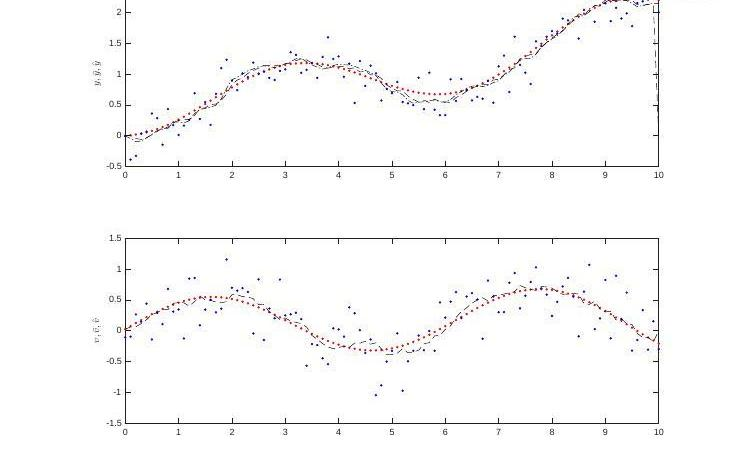
\includegraphics[width=\textwidth]{slide-14.jpg}
  \caption{Complementary / Kalman filter performance on a simulated
    trajectory.
    \textbf{Red (dotted)}: the true deterministic signal.
    \textbf{Blue (dots)}: the noisy raw measurements.
    \textbf{Black (dashed)}: the filter estimate.
    \textbf{Top plot}: position $y$ (or $\hat{y}$) vs.\ time.
    The measurements (blue) scatter widely around the true trajectory
    (red); the filter (black) tracks the true signal closely, smoothing
    out the noise while following the trend.
    \textbf{Bottom plot}: velocity $v$ (or $\dot{\hat{y}}$) vs.\ time.
    The velocity estimate from the filter (black) tracks the true
    velocity (red) while rejecting the measurement scatter.
    Neither position nor velocity is directly measured cleanly at every
    step --- the filter reconstructs both from the combined information.}
\end{figure}

The performance plot shows the fundamental trade-off the time constant
$\tau$ controls:

\begin{itemize}[leftmargin=1.4em, itemsep=3pt]
  \item \textbf{Too small $\tau$} (trusts GPS too much): the estimate
    follows the raw GPS readings closely --- it is noisy and jumpy,
    barely smoother than the blue dots.
    Every GPS error immediately corrupts the estimate.

  \item \textbf{Too large $\tau$} (trusts velocity too much): the estimate
    integrates the velocity sensor for too long without GPS correction ---
    it drifts away from the true position between GPS updates, and can be
    slow to correct when GPS says it is wrong.

  \item \textbf{Correctly tuned $\tau$}: the estimate (black) stays close
    to the true signal (red) --- the GPS prevents long-term drift while
    the velocity sensor provides the fast, smooth dynamics between GPS
    fixes.
    The error is much smaller than the raw measurement noise at all times.
\end{itemize}

\begin{notebox}
  \textbf{How to choose $\tau$ in practice}

  There is no single formula for $\tau$ --- it depends on the relative
  noise levels of your two sensors.
  Two practical guidelines:

  \begin{itemize}[leftmargin=1.2em, itemsep=3pt]
    \item \textbf{Rule of thumb}: set the crossover frequency
      $\omega_c = 1/\tau$ to be in the frequency band where your GPS
      noise and your velocity-integration drift are roughly equal in
      magnitude.
      Below this frequency, GPS is more reliable; above it, velocity
      integration is cleaner.

    \item \textbf{Trial and adjust}: start with a $\tau$ of a few seconds
      (for a GPS + IMU system), simulate or test on real data, and observe
      whether the estimate lags GPS errors (too large $\tau$) or is too
      noisy (too small $\tau$).
      Adjust $\tau$ until the black curve in the performance plot
      approximates the red curve well.
  \end{itemize}

  If you have careful noise models for both sensors (variances and spectral
  densities), use the Kalman filter instead --- it computes the optimal
  crossover automatically from those models and adapts it over time.
  The complementary filter with fixed $\tau$ is optimal only if the noise
  levels stay constant, which in practice they often do not.
\end{notebox}

% ── Key takeaways ─────────────────────────────────────────────────────────────
\begin{keybox}
  \textbf{Section 3 --- Key Takeaways}
  \begin{itemize}[leftmargin=1.2em, itemsep=2pt]
    \item A \textbf{complementary filter} fuses two sensors by splitting
      the frequency spectrum between them:
      $z = F_1(s)\,y_1 + F_2(s)\,y_2$ with $F_1(s) = I - F_2(s)$.
      One sensor covers low frequencies; the other covers high
      frequencies; together they cover everything exactly once.

    \item Choose $F_2(s)$ as a low-pass filter (e.g.\
      $\tfrac{1}{\tau s+1}$) and $F_1(s)$ follows automatically as its
      high-pass complement $\tfrac{\tau s}{\tau s+1}$.

    \item For the velocity+position example:
      $\hat{y} = \tfrac{1}{\tau s+1}(\tau v + y)$.
      GPS prevents drift at low frequencies; velocity integration gives
      smooth, fast updates at high frequencies.
      The time constant $\tau$ sets the crossover between them.

    \item The discrete-time implementation uses the
      \textbf{Tustin (bilinear) approximation} ($s \leftarrow
      \tfrac{2}{T_s}\tfrac{z-1}{z+1}$), giving the recursion:
      \[
        \hat{y}_k = \frac{1}{\alpha_1}
          \bigl(-\alpha_0\hat{y}_{k-1}
          + \beta\tfrac{T_s}{2}v_k
          + \beta\tfrac{T_s}{2}v_{k-1}
          + y_k + y_{k-1}\bigr)
      \]
      with $\alpha_1 = \tfrac{\tau T_s}{2}+1$,\;
      $\alpha_0 = 1-\tfrac{\tau T_s}{2}$,\; $\beta = \tfrac{\tau T_s}{2}$.

    \item The complementary filter is a computationally trivial
      alternative to the Kalman filter when: (1) two sensors split cleanly
      by frequency, and (2) noise levels are roughly constant so a fixed
      $\tau$ is acceptable.
      The KF is preferable when optimal weighting or time-varying noise is
      important.
  \end{itemize}
\end{keybox}

% ==============================================================================
\newpage
\section*{Section 4 \quad Attitude Determination \& Orientation Representation}
% ==============================================================================

So far the lecture has dealt with sensor fusion in the context of quantities
that live in ordinary Euclidean space --- position, velocity, altitude.
We now turn to a different and more geometrically subtle problem:
\textbf{attitude determination} --- estimating the 3D orientation of a rigid
body (a drone, a phone, a robot arm) from sensor measurements.
This is harder than it first appears, both because the sensors are imperfect
in complementary ways, and because orientation itself does not live in a
simple flat space.

% ------------------------------------------------------------------------------
\subsection*{4.1 \quad The Problem --- Why IMU Sensors Alone Are Insufficient}
% ------------------------------------------------------------------------------

\begin{figure}[H]
  \centering
  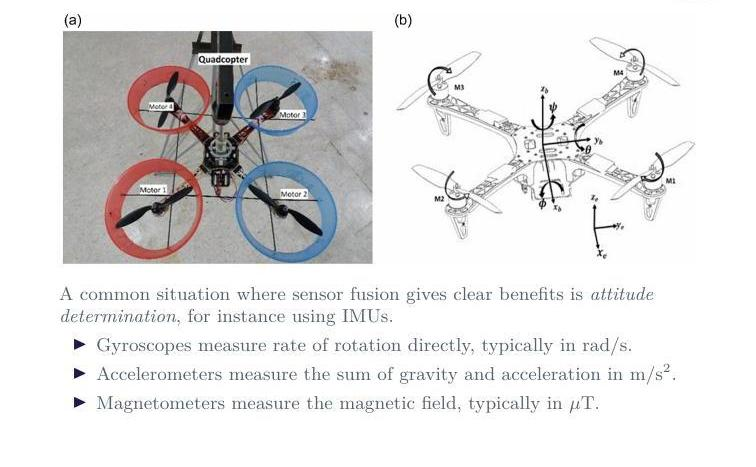
\includegraphics[width=\textwidth]{slide-15.jpg}
  \caption{Attitude determination on a quadcopter.
    \textbf{(a)} Physical quadcopter with four motors.
    \textbf{(b)} Schematic showing the body-fixed axes $(x_b, y_b, z_b)$ and
    the sensors mounted to the frame.
    The goal is to estimate the \textbf{attitude} of the body --- the
    orientation of the body-fixed frame relative to a fixed world frame ---
    from the IMU sensor readings.
    The three sensor types are gyroscopes (angular rate), accelerometers
    (specific force), and magnetometers (magnetic field).}
\end{figure}

An \textbf{Inertial Measurement Unit (IMU)} typically contains three types of
sensor, each measuring a different physical quantity:

\begin{itemize}[leftmargin=1.4em, itemsep=4pt]
  \item \textbf{Gyroscope} --- measures the \emph{angular rate} of the body,
    typically in rad/s.
    Integrating the angular rate gives orientation --- but any small bias in
    the gyroscope reading accumulates over time into a large orientation error
    (\textbf{drift}).
    Good at tracking fast rotations; fails over long time scales without
    correction.

  \item \textbf{Accelerometer} --- measures the \emph{specific force}: the
    vector sum of all non-gravitational forces per unit mass acting on the
    sensor, in m/s$^2$.
    In steady state (hovering, standing still), the accelerometer reads only
    the gravity vector, which points straight down in the world frame.
    The direction of this gravity reading tells you roll and pitch.
    But during any acceleration, the external acceleration adds to gravity
    and corrupts the attitude estimate.

  \item \textbf{Magnetometer} --- measures the ambient magnetic field vector,
    typically in $\mu$T.
    In steady state this vector points approximately toward magnetic north,
    giving a reference for the yaw angle.
    But the magnetometer is sensitive to nearby ferromagnetic objects and
    electric currents (motors, wiring), which can deflect the measured field
    far from the true Earth field.
\end{itemize}

\begin{notebox}
  \textbf{Why each sensor alone is insufficient --- the complementary structure}

  Each sensor has a strength the others lack, and a weakness the others
  compensate for:

  \medskip
  \begin{tabular}{@{} p{2.8cm} p{4.4cm} p{4.4cm} @{}}
    \toprule
    \textbf{Sensor} & \textbf{Strength} & \textbf{Weakness} \\
    \midrule
    Gyroscope &
      Fast, smooth --- tracks rapid rotations with high bandwidth &
      Drifts over time --- any bias integrates into unbounded error \\[4pt]
    Accelerometer &
      Stable long-term gravity reference --- no drift for roll and pitch &
      Corrupted during manoeuvres --- cannot separate gravity from
      linear acceleration \\[4pt]
    Magnetometer &
      Stable long-term yaw reference (magnetic north) --- no drift &
      Disturbed by nearby metal and electronics --- unreliable near
      motors \\
    \bottomrule
  \end{tabular}

  \medskip
  The complementary structure is clear: the gyroscope is reliable at
  \emph{high frequencies} (fast rotations) but fails at low frequencies
  (drift); the accelerometer and magnetometer provide stable
  \emph{low-frequency} references but are corrupted at high frequencies
  (vibration, acceleration).
  This is exactly the complementary-filter split from Section~3, applied
  now to orientation rather than position.
  The Madgwick and Mahoney filters in Sections~6 and~7 exploit this
  structure explicitly.
\end{notebox}

% ------------------------------------------------------------------------------
\subsection*{4.2 \quad Euler Angles --- Describing Orientation with Three
Angles}
% ------------------------------------------------------------------------------

\begin{figure}[H]
  \centering
  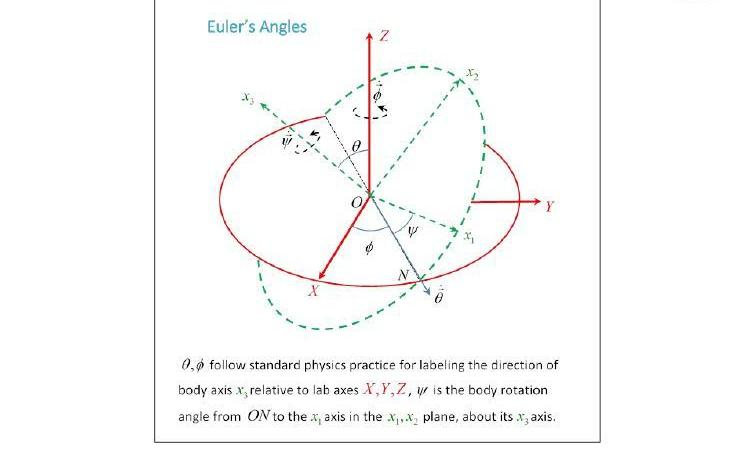
\includegraphics[width=\textwidth]{slide-16.jpg}
  \caption{Euler angles.
    The orientation of the body frame $(x_1, x_2, x_3)$ relative to the
    lab frame $(X, Y, Z)$ is described by three successive rotations.
    \textbf{$\phi$} (roll): rotation about the body $x_1$ axis.
    \textbf{$\theta$} (pitch): rotation about the intermediate $x_2$ axis.
    \textbf{$\psi$} (yaw): the rotation angle from the reference line $ON$
    to the $x_1$ axis in the $x_1$--$x_2$ plane, measured about the $x_3$
    axis.
    The dashed lines show the intermediate frames created by each successive
    rotation.}
\end{figure}

The most intuitive way to describe the orientation of a rigid body in 3D is
with \textbf{Euler angles}: three angles that parameterise three successive
rotations bringing the world frame into alignment with the body frame.

For aerospace and robotics the standard convention is:
\begin{itemize}[leftmargin=1.4em, itemsep=3pt]
  \item \textbf{Roll} $\phi$: rotation about the forward ($x$) axis ---
    tilting left or right.
    Range: $[-180^\circ, 180^\circ]$.
  \item \textbf{Pitch} $\theta$: rotation about the right ($y$) axis ---
    nose up or nose down.
    Range: $[-90^\circ, 90^\circ]$.
  \item \textbf{Yaw} $\psi$: rotation about the vertical ($z$) axis ---
    turning left or right like a compass heading.
    Range: $[-180^\circ, 180^\circ]$.
\end{itemize}

\begin{notebox}
  \textbf{The order of rotations matters --- Euler angles are not commutative}

  Unlike adding numbers, rotations in 3D do not commute.
  Rotating $90^\circ$ about $x$ first then $90^\circ$ about $z$ gives a
  different result than the same rotations in reverse order.
  Euler angles must always be applied in a fixed, agreed-upon sequence.
  The most common convention in aerospace is \textbf{ZYX} (yaw first, then
  pitch, then roll), also called the \emph{Tait-Bryan} convention.
  Always check which convention a paper or datasheet uses --- mixing them
  gives wrong results with no obvious error message.
\end{notebox}

\begin{warnbox}
  \textbf{Gimbal lock --- the fundamental problem with Euler angles}

  Euler angles have a critical failure mode called \textbf{gimbal lock}.
  It occurs when the pitch angle reaches $\pm 90^\circ$ (nose straight up
  or straight down).
  At this configuration, the roll axis and the yaw axis become aligned ---
  two of the three rotations now do the same thing and one degree of freedom
  is lost.

\begin{center}
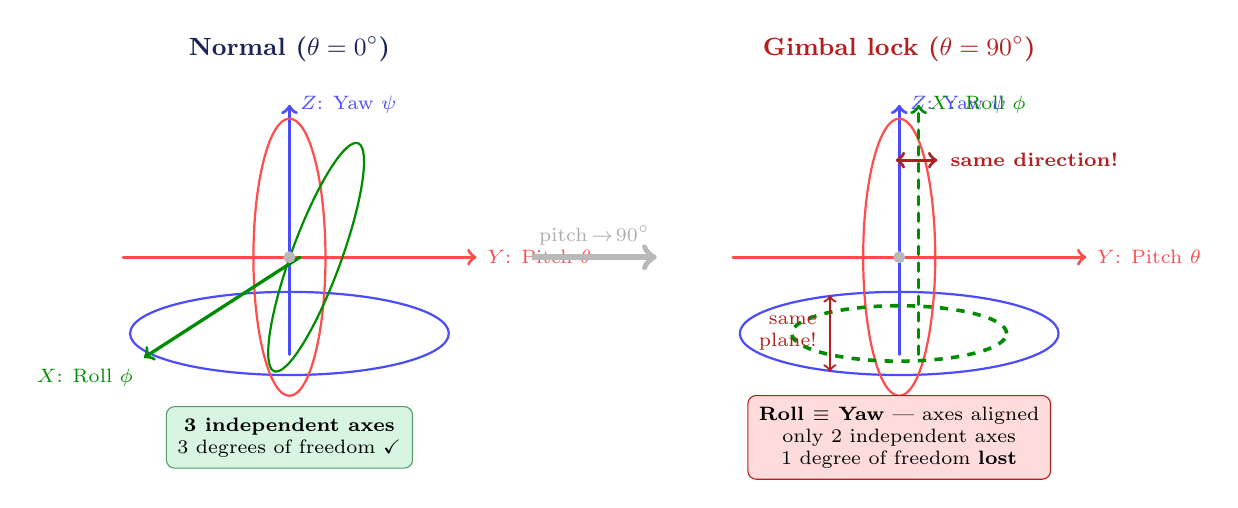
\begin{tikzpicture}[scale=0.88,
    ax/.style={->, very thick, line cap=round}]

%% ── LEFT: Normal operation (pitch = 0°) ──────────────────────────────────────
\begin{scope}[xshift=-4.4cm]
  \node[font=\small\bfseries, color=headernavy] at (0,4.1)
    {Normal ($\theta = 0^\circ$)};

  % Outer ring — lies in horizontal plane, yaw axis = world Z (up)
  \draw[thick, blue!70] (0,0) ellipse (2.3 and 0.60);
  \draw[ax, blue!70] (0,-0.3) -- (0,3.3)
    node[right, font=\scriptsize] {$Z$: Yaw $\psi$};

  % Middle ring — lies in vertical frontal plane, pitch axis = Y (right)
  \draw[thick, red!70] (0,1.1) ellipse (0.52 and 2.0);
  \draw[ax, red!70] (-2.4,1.1) -- (2.7,1.1)
    node[right, font=\scriptsize] {$Y$: Pitch $\theta$};

  % Inner ring — lies in vertical side plane (axis = X, pointing toward viewer)
  % Drawn with xslant to give a sense of depth
  \draw[thick, green!55!black, xslant=0.35] (0,1.1) ellipse (0.38 and 1.65);
  % Roll axis: out of page, shown going lower-left (perspective arrow)
  \draw[ax, green!55!black] (0.15,1.1) -- (-2.1,-0.35)
    node[below left, font=\scriptsize] {$X$: Roll $\phi$};

  \filldraw[gray!55] (0,1.1) circle (2.2pt);

  \node[draw=defgreen!70, fill=defgreenbg, rounded corners=3pt,
        font=\scriptsize, align=center, inner sep=4pt] at (0,-1.5)
    {\textbf{3 independent axes}\\3 degrees of freedom \checkmark};
\end{scope}

%% ── CENTRAL ARROW ────────────────────────────────────────────────────────────
\draw[->, line width=2.2pt, gray!55]
  (-0.9,1.1) -- (0.9,1.1)
  node[midway, above, font=\scriptsize, color=gray!65]
    {pitch $\!\to\! 90^\circ$};

%% ── RIGHT: Gimbal lock (pitch = 90°) ─────────────────────────────────────────
\begin{scope}[xshift=4.4cm]
  \node[font=\small\bfseries, color=warnred] at (0,4.1)
    {Gimbal lock ($\theta = 90^\circ$)};

  % Outer ring — unchanged: horizontal, yaw axis = Z (up)
  \draw[thick, blue!70] (0,0) ellipse (2.3 and 0.60);
  \draw[ax, blue!70] (0,-0.3) -- (0,3.3)
    node[right, font=\scriptsize] {$Z$: Yaw $\psi$};

  % Middle ring — pitch axis still = Y (unchanged, it's the axis we just rotated about)
  \draw[thick, red!70] (0,1.1) ellipse (0.52 and 2.0);
  \draw[ax, red!70] (-2.4,1.1) -- (2.7,1.1)
    node[right, font=\scriptsize] {$Y$: Pitch $\theta$};

  % Inner ring — after 90° pitch, it has FALLEN into the horizontal plane
  % i.e. same plane as the OUTER ring  →  draw as a slightly smaller horizontal ellipse
  \draw[thick, green!55!black, dashed, line width=1.3pt]
    (0,0) ellipse (1.55 and 0.40);
  % Roll axis now also points VERTICALLY — same direction as Yaw!
  \draw[ax, green!55!black, dashed] (0.28,-0.3) -- (0.28,3.3)
    node[right, font=\scriptsize, green!55!black] {$X$: Roll $\phi$};

  % ALIGNED call-out
  \draw[warnred, very thick, <->] (-0.05,2.5) -- (0.55,2.5);
  \node[warnred, font=\scriptsize\bfseries, right] at (0.6,2.5)
    {same direction!};

  % Highlight that inner ring and outer ring are now co-planar
  \draw[warnred, thick, <->] (-1.0,-0.55) -- (-1.0,0.55);
  \node[warnred, font=\scriptsize, left, align=right] at (-1.05,0.0)
    {same\\plane!};

  \filldraw[gray!55] (0,1.1) circle (2.2pt);

  \node[draw=warnred, fill=warnredbg, rounded corners=3pt,
        font=\scriptsize, align=center, inner sep=4pt] at (0,-1.5)
    {\textbf{Roll $\equiv$ Yaw} --- axes aligned\\only 2 independent axes\\
     1 degree of freedom \textbf{lost}};
\end{scope}

\end{tikzpicture}
\end{center}

  In practice this means:
  \begin{itemize}[leftmargin=1.2em, itemsep=2pt]
    \item The Euler angle representation becomes \textbf{singular} ---
      infinitely many $(\phi, \theta, \psi)$ combinations describe the same
      physical orientation.
    \item \textbf{Numerical derivatives blow up} --- the kinematic equations
      relating angular velocity $\omega$ to $(\dot\phi, \dot\theta, \dot\psi)$
      contain $1/\cos\theta$ terms which diverge as $\theta \to \pm90^\circ$.
    \item Any filter propagating Euler angles will fail or produce nonsense
      near this singularity.
  \end{itemize}

  For a drone doing aerobatics, a robot arm that can reach above its head,
  or any system that passes through $\theta = \pm90^\circ$, Euler angles
  are unsuitable.
  \textbf{Quaternions} (Section~4.3) were developed specifically to avoid
  this singularity.
\end{warnbox}

% ------------------------------------------------------------------------------
\subsection*{4.3 \quad Quaternions --- A Singularity-Free Representation}
% ------------------------------------------------------------------------------

A quaternion is a 4-element vector that encodes any 3D rotation as one
\textbf{rotation axis} $\hat{n}$ and one \textbf{rotation angle} $\alpha$:
\[
  \mathbf{q}
  = \begin{bmatrix} q_0 \\ \vec{q} \end{bmatrix}
  = \begin{bmatrix} q_0 \\ q_x \\ q_y \\ q_z \end{bmatrix}
  = \begin{bmatrix} \cos(\alpha/2) \\ \sin(\alpha/2)\,n_x \\
                    \sin(\alpha/2)\,n_y \\ \sin(\alpha/2)\,n_z \end{bmatrix}
  \in \mathbb{R}^4
\]
The scalar part $q_0$ encodes how large the rotation is; the vector part
$\vec{q}$ encodes which axis it is about.
For it to represent a pure rotation (no scaling), we \textbf{define and
enforce} the unit-length constraint:
\[
  \|\mathbf{q}\| = \sqrt{q_0^2 + q_x^2 + q_y^2 + q_z^2} = 1
\]
This is not automatically true --- it is a requirement we impose by
construction.
When we build $\mathbf{q}$ from an axis $\hat{n}$ and angle $\alpha$ using
the formula above, the result satisfies $\|\mathbf{q}\|=1$ exactly
(because $\cos^2(\alpha/2) + \sin^2(\alpha/2) = 1$).
But when a filter integrates the quaternion numerically over time, floating-
point rounding slowly pushes the norm away from 1.
The fix is a periodic one-line renormalisation:
\[
  \mathbf{q} \;\leftarrow\; \frac{\mathbf{q}}{\|\mathbf{q}\|}
\]
Without this step the quaternion drifts off the unit sphere and stops
representing a valid rotation.

\begin{notebox}
  \textbf{Concrete example --- what do the four numbers actually mean?}

  \begin{center}
    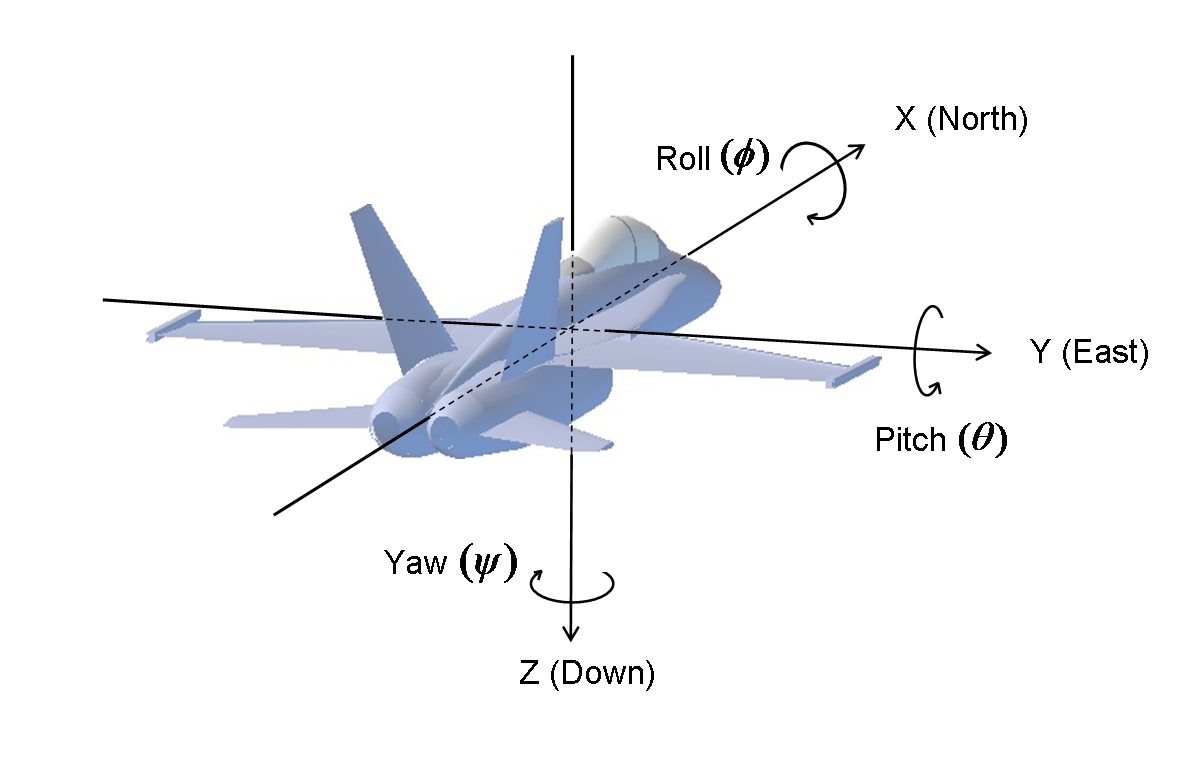
\includegraphics[width=0.72\textwidth]{euler_axes.png}
  \end{center}

  Suppose a drone needs to rotate $90^\circ$ about the world $z$-axis
  (a pure yaw turn).
  The rotation axis is $\hat{n} = (0, 0, 1)$ and the angle is
  $\alpha = 90^\circ$.
  Plugging in:
  \[
    \mathbf{q}
    = \begin{bmatrix}
        \cos(45^\circ) \\ \sin(45^\circ)\cdot 0 \\
        \sin(45^\circ)\cdot 0 \\ \sin(45^\circ)\cdot 1
      \end{bmatrix}
    = \begin{bmatrix}
        \tfrac{\sqrt{2}}{2} \\ 0 \\ 0 \\ \tfrac{\sqrt{2}}{2}
      \end{bmatrix}
    \approx \begin{bmatrix} 0.707 \\ 0 \\ 0 \\ 0.707 \end{bmatrix}
  \]
  Reading the four numbers:
  \begin{itemize}[leftmargin=1.2em, itemsep=2pt]
    \item $q_x = 0$, $q_y = 0$: no $x$ or $y$ component in the axis ---
      pure $z$-axis rotation.
    \item $q_z = 0.707 = \sin(45^\circ)$: the rotation axis points entirely
      along $z$ (yaw axis).
    \item $q_0 = 0.707 = \cos(45^\circ)$: see below --- this is the
      confusing part.
  \end{itemize}
  Verify unit norm: $0.707^2 + 0^2 + 0^2 + 0.707^2 = 0.5 + 0.5 = 1$
  \checkmark

  \textbf{Why does $q_0 = 0.707$ mean $90^\circ$, and $q_0 = 0$ mean
  $180^\circ$?}
  This trips everyone up because $q_0$ works \emph{backwards} from
  what feels natural.
  $q_0 = \cos(\alpha/2)$, and cosine \emph{decreases} as the angle grows:
  the bigger the rotation, the \emph{smaller} $q_0$ gets.

  Think of it with a barrel roll.
  You start level ($0^\circ$ roll, $q_0 = 1$).
  As you roll over, $q_0$ falls.
  When you are completely upside-down ($180^\circ$ roll), $q_0 = 0$.
  That is the most ``different'' orientation from level --- not zero
  rotation, but the \emph{maximum}.
  Roll all the way back to level ($360^\circ$) and $q_0$ reaches $-1$,
  then the sign flips back to $+1$ at the next full turn.

  \medskip
  \begin{center}
  \begin{tabular}{@{} l c c @{}}
    \toprule
    Situation & $\alpha$ & $q_0 = \cos(\alpha/2)$ \\
    \midrule
    Not rotated at all (identity) & $0^\circ$   & $1$    \\
    Quarter turn                  & $90^\circ$  & $0.707$\\
    Half turn --- fully flipped   & $180^\circ$ & $0$    \\
    Full turn --- back to start   & $360^\circ$ & $-1$   \\
    \bottomrule
  \end{tabular}
  \end{center}

  \medskip
  So $q_0$ is a measure of \textbf{how close to the identity} you are:
  $q_0 = 1$ means sitting still, $q_0 = 0$ means halfway around,
  $q_0 = -1$ means a full turn with a sign flip.

  The three reference quaternions (all yaw rotations, axis $= z$):
  \[
    \mathbf{q}_{90^\circ}
    = \begin{bmatrix} 0.707 \\ 0 \\ 0 \\ 0.707 \end{bmatrix}, \quad
    \mathbf{q}_{180^\circ}
    = \begin{bmatrix} 0 \\ 0 \\ 0 \\ 1 \end{bmatrix}, \quad
    \mathbf{q}_\text{identity}
    = \begin{bmatrix} 1 \\ 0 \\ 0 \\ 0 \end{bmatrix}
  \]

  \textbf{Why $\alpha/2$ and not $\alpha$?}
  In the rotation formula $\mathbf{v}' = \mathbf{q}\otimes\mathbf{v}
  \otimes\mathbf{q}^*$ (Section~4.5), $\mathbf{q}$ acts twice ---
  left and right.
  Each application contributes $\alpha/2$; together they give $\alpha$.
  Storing $\alpha$ directly would produce a double rotation.
\end{notebox}

\begin{warnbox}
  \textbf{$q_0$ works backwards --- bigger rotation means smaller $q_0$}

  $q_0 = \cos(\alpha/2)$ \emph{decreases} as the rotation grows.
  The bigger the rotation, the smaller $q_0$ gets --- not the larger.

  Think of a barrel roll: you start level ($q_0 = 1$).
  As you roll over, $q_0$ falls.
  Completely upside-down ($180^\circ$): $q_0 = 0$ --- the most
  ``different'' orientation from level.
  Back to level after a full $360^\circ$: $q_0 = -1$, sign-flipped.

  \textbf{Does the filter reset $q_0$ back to 1 after a full turn?}
  No --- never.
  $(-1, 0, 0, 0)$ and $(1, 0, 0, 0)$ are physically identical
  (same orientation, just opposite sign).
  The filter keeps running continuously; no reset happens.

  \textbf{Sitting still} = quaternion not changing over time,
  regardless of what the four numbers are.
  A quaternion frozen at $(-1, 0, 0, 0)$ means sitting still at the
  reference orientation.
  A quaternion frozen at $(0.707, 0, 0, 0.707)$ means sitting still at
  $90^\circ$ yaw from reference.
\end{warnbox}

\begin{warnbox}
  \textbf{$(1,0,0,0)$ is not a fixed physical direction --- it is
  relative to your initial state}

  The identity quaternion does not mean ``level'', ``pointing north'',
  or any fixed world direction.
  It simply means \textbf{no rotation from wherever the filter started}.

  \begin{itemize}[leftmargin=1.2em, itemsep=2pt]
    \item Start level, pointing north $\to$ $(1,0,0,0)$ means level
      and pointing north.
    \item Start pointing straight up $\to$ $(1,0,0,0)$ means pointing
      straight up.
    \item Start banked $45^\circ$ right $\to$ $(1,0,0,0)$ means banked
      $45^\circ$ right.
  \end{itemize}

  All three read $(1,0,0,0)$ but describe completely different physical
  orientations.
  This is why IMU filters must be \textbf{initialised carefully} ---
  whatever orientation the body is in when the filter starts becomes
  the reference that all subsequent quaternions are measured against.
\end{warnbox}

\begin{figure}[H]
  \centering
  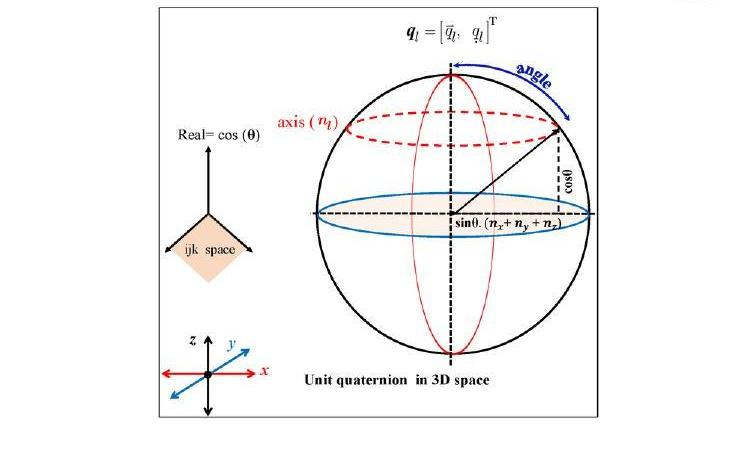
\includegraphics[width=\textwidth]{slide-17.jpg}
  \caption{Unit quaternion sphere.
    Every point on the surface of this sphere is one specific 3D rotation.
    \textbf{Vertical axis} (Real $= q_0 = \cos(\alpha/2)$): encodes the
    rotation size --- top ($q_0=1$) is the identity (no rotation), equator
    ($q_0=0$) is a $180^\circ$ half-turn, bottom ($q_0=-1$) is a full
    $360^\circ$ turn (same physical orientation as the identity, but
    negated quaternion).
    \textbf{Horizontal disc} (ijk space): the 3D space of the imaginary
    part $\vec{q}$ --- the direction in this disc is the rotation axis
    $\eta_l$, and the distance from the centre is $\sin(\alpha/2)$.
    \textbf{Opposite points} $\mathbf{q}$ and $-\mathbf{q}$ always
    represent the same physical rotation --- every orientation has two
    quaternion representations.}
\end{figure}

\begin{notebox}
  \textbf{Why quaternions avoid gimbal lock}

  Euler angles use 3 numbers for 3D orientation.
  The problem: the space of all 3D rotations ($SO(3)$) cannot be covered by
  3 smooth coordinates without at least one singularity --- gimbal lock is
  that unavoidable breakdown.

  Unit quaternions use 4 numbers with 1 constraint ($\|\mathbf{q}\|=1$),
  giving 3 effective free parameters --- same count as Euler angles, but
  the constraint surface is a smooth sphere with no singular points anywhere.
  Integration through any orientation works cleanly.
  The only housekeeping needed: renormalise $\mathbf{q} \leftarrow
  \mathbf{q}/\|\mathbf{q}\|$ periodically, since numerical drift slowly
  pushes the quaternion off the unit sphere.
\end{notebox}

% ------------------------------------------------------------------------------
\subsection*{4.4 \quad Converting Quaternions to Euler Angles}
% ------------------------------------------------------------------------------

\begin{figure}[H]
  \centering
  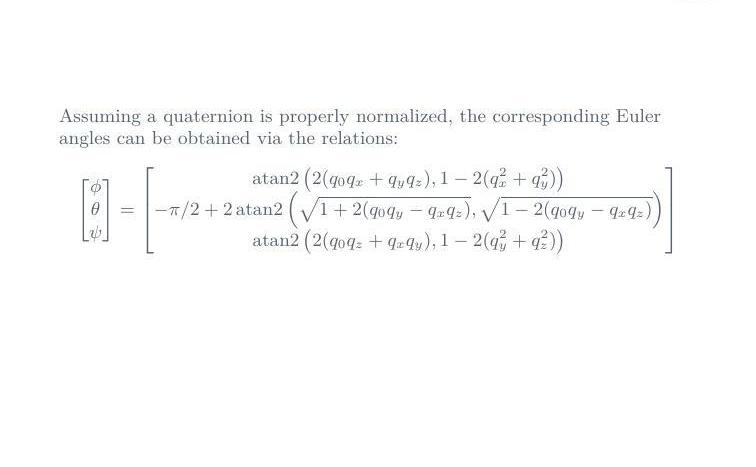
\includegraphics[width=\textwidth]{slide-19.jpg}
  \caption{Quaternion-to-Euler conversion.
    Given a unit quaternion $(q_0, q_x, q_y, q_z)$, the corresponding ZYX
    Tait-Bryan Euler angles (roll $\phi$, pitch $\theta$, yaw $\psi$) are
    recovered by three \texttt{atan2} expressions.
    The filters in Sections~6 and~7 work in quaternion space internally;
    Euler angles are only computed here at the output for display.}
\end{figure}

The attitude filters work internally with quaternions.
For human-readable output the quaternion is converted to Euler angles once at
the end:
\[
  \begin{bmatrix} \phi \\ \theta \\ \psi \end{bmatrix}
  =
  \begin{bmatrix}
    \mathrm{atan2}\!\bigl(2(q_0 q_x + q_y q_z),\;
      1 - 2(q_x^2 + q_y^2)\bigr) \\[6pt]
    -\tfrac{\pi}{2} + 2\,\mathrm{atan2}\!\bigl(
      \sqrt{1 + 2(q_0 q_y - q_x q_z)},\;
      \sqrt{1 - 2(q_0 q_y - q_x q_z)}\bigr) \\[6pt]
    \mathrm{atan2}\!\bigl(2(q_0 q_z + q_x q_y),\;
      1 - 2(q_y^2 + q_z^2)\bigr)
  \end{bmatrix}
\]

\begin{center}
\begin{tabular}{@{} l p{2.8cm} p{8.0cm} @{}}
  \toprule
  Symbol & Name & Meaning \\
  \midrule
  $\phi$ & Roll &
    Rotation about the body $x$-axis (forward axis).
    Positive = right side down. \\[3pt]
  $\theta$ & Pitch &
    Rotation about the body $y$-axis (right axis).
    Positive = nose up. \\[3pt]
  $\psi$ & Yaw &
    Rotation about the body $z$-axis (down axis).
    Positive = clockwise from above. \\[3pt]
  $\mathrm{atan2}(y,x)$ & Four-quadrant arctangent &
    Returns the angle in $(-\pi, \pi]$ whose tangent is $y/x$, using
    the signs of both arguments to choose the correct quadrant.
    Handles $x = 0$ cleanly and covers the full $360^\circ$ range,
    unlike $\arctan(y/x)$. \\
  \bottomrule
\end{tabular}
\end{center}

\begin{notebox}
  \textbf{Which quaternion components control which angle}

  Each Euler angle is extracted from a different subset of quaternion
  components, determined by which body axis it rotates about:

  \begin{itemize}[leftmargin=1.2em, itemsep=3pt]
    \item \textbf{Roll $\phi$}: terms $q_0 q_x$ and $q_y q_z$ both involve
      $q_x$ --- the imaginary component along the rotation axis for roll
      ($x$-axis).
    \item \textbf{Pitch $\theta$}: term $q_0 q_y - q_x q_z$ involves $q_y$
      --- the $y$-axis component.
      The double-\texttt{atan2} with square roots replaces a simple
      $\arcsin$ to avoid the $\pm90^\circ$ discontinuity that would
      otherwise appear at the boundary of the arcsin range.
    \item \textbf{Yaw $\psi$}: terms $q_0 q_z$ and $q_x q_y$ involve $q_z$
      --- the $z$-axis component.
  \end{itemize}

  This is useful for debugging: if yaw suddenly goes wrong while roll and
  pitch are fine, the error is in the $q_z$ component of your quaternion.
  In practice use a library function (\texttt{quat2eul} in MATLAB) ---
  knowing the structure tells you which component to inspect, not how to
  reimplement the formula.
\end{notebox}

% ------------------------------------------------------------------------------
\subsection*{4.5 \quad Rotating a Vector with a Quaternion}
% ------------------------------------------------------------------------------

\begin{figure}[H]
  \centering
  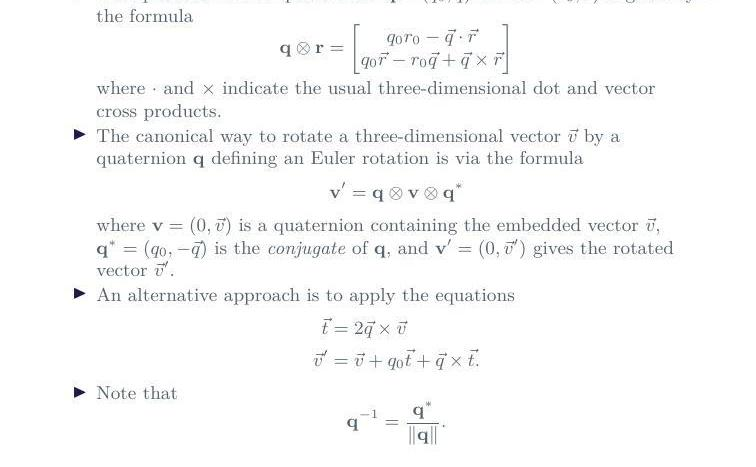
\includegraphics[width=\textwidth]{slide-20.jpg}
  \caption{Quaternion multiplication and rotation.
    \textbf{Top}: the general quaternion product
    $\mathbf{q}\otimes\mathbf{r}$.
    \textbf{Middle}: rotating vector $\vec{v}$ by $\mathbf{q}$ via
    $\mathbf{v}' = \mathbf{q}\otimes\mathbf{v}\otimes\mathbf{q}^*$.
    \textbf{Bottom}: the efficient two-cross-product alternative that avoids
    computing two full quaternion products.
    \textbf{Far right}: the quaternion inverse $\mathbf{q}^{-1} =
    \mathbf{q}^*/\|\mathbf{q}\|$.}
\end{figure}

\textbf{Quaternion multiplication.}

Given two quaternions written out in full:
\[
  \mathbf{q}
  = \begin{bmatrix} q_0 \\ q_x \\ q_y \\ q_z \end{bmatrix},
  \qquad
  \mathbf{r}
  = \begin{bmatrix} r_0 \\ r_x \\ r_y \\ r_z \end{bmatrix}
\]
their product is:
\[
  \mathbf{q} \otimes \mathbf{r}
  = \begin{bmatrix}
      q_0 r_0 - \vec{q}\cdot\vec{r} \\
      q_0\vec{r} + r_0\vec{q} + \vec{q}\times\vec{r}
    \end{bmatrix}
  = \begin{bmatrix}
      q_0 r_0 - q_x r_x - q_y r_y - q_z r_z \\
      q_0 r_x + q_x r_0 + q_y r_z - q_z r_y \\
      q_0 r_y - q_x r_z + q_y r_0 + q_z r_x \\
      q_0 r_z + q_x r_y - q_y r_x + q_z r_0
    \end{bmatrix}
\]

\begin{center}
\begin{tabular}{@{} l p{3.0cm} p{7.5cm} @{}}
  \toprule
  Symbol & Name & Meaning \\
  \midrule
  $\otimes$ & Quaternion product &
    Non-commutative: $\mathbf{q}\otimes\mathbf{r} \neq
    \mathbf{r}\otimes\mathbf{q}$ in general, just like matrix
    multiplication. \\[3pt]
  $\vec{q}\cdot\vec{r}$ & Dot product &
    $q_x r_x + q_y r_y + q_z r_z$ --- scalar. \\[3pt]
  $\vec{q}\times\vec{r}$ & Cross product &
    $(q_y r_z - q_z r_y,\; q_z r_x - q_x r_z,\; q_x r_y - q_y r_x)^\top$
    --- vector, anti-symmetric: $\vec{q}\times\vec{r} = -\vec{r}\times
    \vec{q}$.
    This anti-symmetry is why $\otimes$ is non-commutative. \\
  \bottomrule
\end{tabular}
\end{center}

\textbf{Rotating a vector with a quaternion.}

To rotate 3D vector $\vec{v}$ by the rotation encoded in unit quaternion
$\mathbf{q}$, first form three quaternions side by side:
\[
  \mathbf{q}
  = \begin{bmatrix} q_0 \\ q_x \\ q_y \\ q_z \end{bmatrix},
  \qquad
  \mathbf{v}
  = \begin{bmatrix} 0 \\ v_x \\ v_y \\ v_z \end{bmatrix},
  \qquad
  \mathbf{q}^*
  = \begin{bmatrix} q_0 \\ -q_x \\ -q_y \\ -q_z \end{bmatrix}
\]
$\mathbf{v}$ is the vector embedded as a \textbf{pure quaternion} (zero scalar
part). $\mathbf{q}^*$ is the \textbf{conjugate} of $\mathbf{q}$: same scalar,
negated vector part.
Then apply the double product:
\[
  \mathbf{v}' = \mathbf{q} \otimes \mathbf{v} \otimes \mathbf{q}^*
  \quad\Longrightarrow\quad
  \mathbf{v}'
  = \begin{bmatrix} 0 \\ v_x' \\ v_y' \\ v_z' \end{bmatrix}
\]
The result $\mathbf{v}'$ is also a pure quaternion; its vector part
$(v_x', v_y', v_z')$ is the rotated vector.

\begin{notebox}
  \textbf{Why the double product gives the correct rotation}

  For a unit quaternion, the conjugate equals the inverse:
  $\mathbf{q}^* = \mathbf{q}^{-1}$, so
  $\mathbf{q}\otimes\mathbf{q}^* = (1,\vec{0})$ (identity).
  The double-sided product $\mathbf{q}\otimes\mathbf{v}\otimes\mathbf{q}^*$
  is an algebraic \emph{conjugation} with three guaranteed properties:
  \begin{itemize}[leftmargin=1.2em, itemsep=2pt]
    \item If $\mathbf{v}$ is pure (zero scalar), so is $\mathbf{v}'$ ---
      the scalar cancels.
      The output is always a valid 3D vector.
    \item The magnitude is preserved: $|\vec{v}'| = |\vec{v}|$ ---
      pure rotation, no scaling.
    \item The rotation angle is exactly $\alpha$: each factor contributes
      $\alpha/2$, together giving $\alpha$.
  \end{itemize}

  \textbf{Example --- rotate $\vec{v} = (1,0,0)^\top$ by $90^\circ$ about
  $\hat{z}$:}

  \begin{center}
  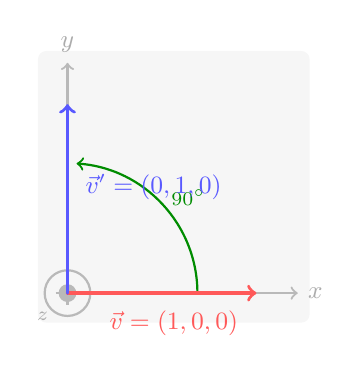
\begin{tikzpicture}[scale=1.5]
    % Background plane
    \fill[gray!7, rounded corners=3pt] (-0.25,-0.25) rectangle (2.05,2.05);

    % Axes
    \draw[->, thick, gray!55] (-0.1,0) -- (1.95,0)
      node[right, font=\small, gray!65] {$x$};
    \draw[->, thick, gray!55] (0,-0.1) -- (0,1.95)
      node[above, font=\small, gray!65] {$y$};

    % z out of page symbol at origin
    \draw[thick, gray!55] (0,0) circle (5.5pt);
    \filldraw[gray!55] (0,0) circle (2pt);
    \node[font=\scriptsize, gray!65, below left] at (-0.08,-0.08) {$z$};

    % 90° arc
    \draw[->, thick, green!55!black] (1.1,0) arc (0:86:1.1)
      node[pos=0.55, right=2pt, font=\scriptsize\bfseries, green!55!black]
      {$90^\circ$};

    % Original vector v = (1,0,0)
    \draw[->, very thick, red!65, line cap=round] (0,0) -- (1.6,0);
    \node[red!65, font=\small, below=3pt] at (0.9,0)
      {$\vec{v}=(1,0,0)$};

    % Rotated vector v' = (0,1,0)
    \draw[->, very thick, blue!65, line cap=round] (0,0) -- (0,1.6);
    \node[blue!65, font=\small, right=3pt] at (0,0.9)
      {$\vec{v}'=(0,1,0)$};
  \end{tikzpicture}
  \end{center}

  The three quaternions involved:
  \[
    \mathbf{q}
    = \begin{bmatrix} \cos 45^\circ \\ 0 \\ 0 \\ \sin 45^\circ \end{bmatrix}
    = \begin{bmatrix} 0.707 \\ 0 \\ 0 \\ 0.707 \end{bmatrix},
    \qquad
    \mathbf{v}
    = \begin{bmatrix} 0 \\ 1 \\ 0 \\ 0 \end{bmatrix},
    \qquad
    \mathbf{q}^*
    = \begin{bmatrix} 0.707 \\ 0 \\ 0 \\ -0.707 \end{bmatrix}
  \]
  Computing $\mathbf{q}\otimes\mathbf{v}\otimes\mathbf{q}^*$ gives:
  \[
    \mathbf{v}'
    = \begin{bmatrix} 0 \\ 0 \\ 1 \\ 0 \end{bmatrix}
    \quad\Longrightarrow\quad
    \vec{v}' = (0,1,0)^\top
  \]
  The red vector along $x$ rotated $90^\circ$ about $z$ and now points
  along $y$ (blue). Correct.
\end{notebox}

\textbf{Efficient alternative rotation formula.}

Two full quaternion products is expensive on embedded hardware.
Given:
\[
  \mathbf{q} = \begin{bmatrix} q_0 \\ \vec{q} \end{bmatrix}, \qquad
  \vec{v} = \begin{bmatrix} v_x \\ v_y \\ v_z \end{bmatrix}
\]
An equivalent formula using only vector operations:
\[
  \vec{\ell} = 2\,\vec{q} \times \vec{v},
  \qquad
  \vec{v}' = \vec{v} + q_0\,\vec{\ell} + \vec{q} \times \vec{\ell}
\]
Two cross products and a few additions --- preferred in real-time
embedded implementations.

\textbf{Verification with the same example}
($\vec{v} = (1,0,0)^\top$, $90^\circ$ about $z$, so
$q_0 = 0.707$, $\vec{q} = (0,\,0,\,0.707)$):

\textit{Step 1} --- compute $\vec{\ell}$:
\[
  \vec{q} \times \vec{v}
  = \begin{bmatrix}0\\0\\0.707\end{bmatrix}
    \times
    \begin{bmatrix}1\\0\\0\end{bmatrix}
  = \begin{bmatrix}
      0\cdot0 - 0.707\cdot0 \\
      0.707\cdot1 - 0\cdot0 \\
      0\cdot0 - 0\cdot1
    \end{bmatrix}
  = \begin{bmatrix}0\\0.707\\0\end{bmatrix}
  \quad\Longrightarrow\quad
  \vec{\ell} = 2\begin{bmatrix}0\\0.707\\0\end{bmatrix}
             = \begin{bmatrix}0\\1.414\\0\end{bmatrix}
\]

\textit{Step 2} --- compute $\vec{v}'$:
\[
  q_0\,\vec{\ell}
  = 0.707\begin{bmatrix}0\\1.414\\0\end{bmatrix}
  = \begin{bmatrix}0\\1\\0\end{bmatrix}
\]
\[
  \vec{q}\times\vec{\ell}
  = \begin{bmatrix}0\\0\\0.707\end{bmatrix}
    \times
    \begin{bmatrix}0\\1.414\\0\end{bmatrix}
  = \begin{bmatrix}
      0\cdot0-0.707\cdot1.414\\
      0.707\cdot0-0\cdot0\\
      0\cdot1.414-0\cdot0
    \end{bmatrix}
  = \begin{bmatrix}-1\\0\\0\end{bmatrix}
\]
\[
  \vec{v}'
  = \vec{v} + q_0\vec{\ell} + \vec{q}\times\vec{\ell}
  = \begin{bmatrix}1\\0\\0\end{bmatrix}
  + \begin{bmatrix}0\\1\\0\end{bmatrix}
  + \begin{bmatrix}-1\\0\\0\end{bmatrix}
  = \begin{bmatrix}0\\1\\0\end{bmatrix} \checkmark
\]
Same result as the double-product method --- $(0,1,0)^\top$ as expected.

\textbf{Quaternion inverse.}

Given:
\[
  \mathbf{q}
  = \begin{bmatrix} q_0 \\ q_x \\ q_y \\ q_z \end{bmatrix}
\]
For any quaternion:
\[
  \mathbf{q}^{-1} = \frac{\mathbf{q}^*}{\|\mathbf{q}\|}
  = \frac{1}{\|\mathbf{q}\|}
  \begin{bmatrix} q_0 \\ -q_x \\ -q_y \\ -q_z \end{bmatrix}
\]
For a unit quaternion ($\|\mathbf{q}\|=1$, which always is given our contraint that it needs to be from earlier), this simplifies to:
\[
  \mathbf{q}^{-1} = \mathbf{q}^*
  = \begin{bmatrix} q_0 \\ -q_x \\ -q_y \\ -q_z \end{bmatrix}
\]
The inverse represents the \emph{opposite} rotation: if $\mathbf{q}$ rotates
the world frame into the body frame, $\mathbf{q}^{-1}$ rotates back.

\begin{warnbox}
  \textbf{Common misconception --- $180^\circ + 180^\circ$ does not mean
  a double rotation}

  It is tempting to think that rotating $180^\circ$ about $y$ and then
  $180^\circ$ about $z$ results in a total of \(||\mathbf{q}||=2\)
  \textbf{This is wrong.}
  Rotations in 3D do not add like numbers --- they compose, and the result
  depends on the axes involved.

  The three quaternions involved:
  \[
    \mathbf{q}_y
    = \begin{bmatrix}0\\0\\1\\0\end{bmatrix}
    \quad\text{(180° about }y\text{)}
    \qquad
    \mathbf{q}_z
    = \begin{bmatrix}0\\0\\0\\1\end{bmatrix}
    \quad\text{(180° about }z\text{)}
  \]
  Computing the composition $\mathbf{q}_y \otimes \mathbf{q}_z$
  (apply $z$ first, then $y$):
  \[
    \mathbf{q}_y \otimes \mathbf{q}_z
    =
    \begin{bmatrix}
      0{\cdot}0 - 0{\cdot}0 - 1{\cdot}0 - 0{\cdot}1 \\
      0{\cdot}0 + 0{\cdot}0 + 1{\cdot}1 - 0{\cdot}0 \\
      0{\cdot}0 - 0{\cdot}1 + 1{\cdot}0 + 0{\cdot}0 \\
      0{\cdot}1 + 0{\cdot}0 - 1{\cdot}0 + 0{\cdot}0
    \end{bmatrix}
    =
    \begin{bmatrix}0\\1\\0\\0\end{bmatrix}
    \quad\text{(180° about }x\text{)}
  \]

  All three side by side:
  \[
    \underbrace{\begin{bmatrix}0\\0\\0\\1\end{bmatrix}}_{\text{180° about }z}
    \qquad
    \underbrace{\begin{bmatrix}0\\0\\1\\0\end{bmatrix}}_{\text{180° about }y}
    \qquad
    \underbrace{\begin{bmatrix}0\\1\\0\\0\end{bmatrix}}_{\text{180° about }y\text{ then }z}
  \]

  All three have $q_0 = 0$ --- all three are $180^\circ$ rotations.
  The vector part $(q_x, q_y, q_z)$ tells you \emph{which} axis:
  the two separate $180^\circ$ rotations composed into a \emph{third}
  $180^\circ$ rotation, this time about the $x$-axis.
  The quaternion only stores the final equivalent result --- it has no
  memory of how many steps were taken to get there.
\end{warnbox}

% ── Key takeaways ─────────────────────────────────────────────────────────────
\begin{keybox}
  \textbf{Section 4 --- Key Takeaways}
  \begin{itemize}[leftmargin=1.2em, itemsep=2pt]
    \item IMU attitude estimation needs \textbf{three sensor types}:
      gyroscope (fast, drifts), accelerometer (gravity reference, disturbed
      by manoeuvres), magnetometer (yaw reference, disturbed by magnetic
      fields).
      Each covers the other's weakness --- the same complementary structure
      as Section~3, applied to orientation.

    \item \textbf{Euler angles} $(\phi, \theta, \psi)$: intuitive but suffer
      from \textbf{gimbal lock} at $\theta = \pm90^\circ$ where two rotation
      axes align, the representation is singular and numerical derivatives
      diverge.

    \item \textbf{Unit quaternions} $\mathbf{q} = (q_0, \vec{q}) \in
      \mathbb{R}^4$, $\|\mathbf{q}\|=1$: rotation of angle $\alpha$ about
      unit axis $\hat{n}$ is $\mathbf{q} = (\cos(\alpha/2),\;
      \sin(\alpha/2)\,\hat{n})$.
      No singularity at any orientation.

    \item \textbf{Quaternion-to-Euler}: three \texttt{atan2} expressions.
      Filters run in quaternion space; Euler angles computed at output only.

    \item \textbf{Quaternion product}:
      $\mathbf{q}\otimes\mathbf{r} = (q_0 r_0 - \vec{q}\cdot\vec{r},\;\;
      q_0\vec{r} + r_0\vec{q} + \vec{q}\times\vec{r})$.
      Non-commutative --- order matters.

    \item \textbf{Rotating} $\vec{v}$ by $\mathbf{q}$:
      $\mathbf{v}' = \mathbf{q}\otimes\mathbf{v}\otimes\mathbf{q}^*$,
      or efficiently:
      $\vec{\ell} = 2\vec{q}\times\vec{v}$,\;
      $\vec{v}' = \vec{v} + q_0\vec{\ell} + \vec{q}\times\vec{\ell}$.

    \item For unit quaternions: $\mathbf{q}^{-1} = \mathbf{q}^* =
      (q_0, -\vec{q})$.
  \end{itemize}
\end{keybox}

% ==============================================================================
\newpage
\section*{Section 5 \quad IMU Measurement Models \& Quaternion Kinematics}
% ==============================================================================

We now have the mathematical tools for representing orientation as a
quaternion.
This section builds the \emph{models} that connect the IMU sensor readings to
that quaternion --- the gyroscope model that drives the quaternion forward in
time, and the accelerometer/magnetometer models that provide correction
references.
These models are the inputs to the Madgwick and Mahoney filters in
Sections~6 and~7.

% ------------------------------------------------------------------------------
\subsection*{5.1 \quad IMU Measurement Models}
% ------------------------------------------------------------------------------

\begin{figure}[H]
  \centering
  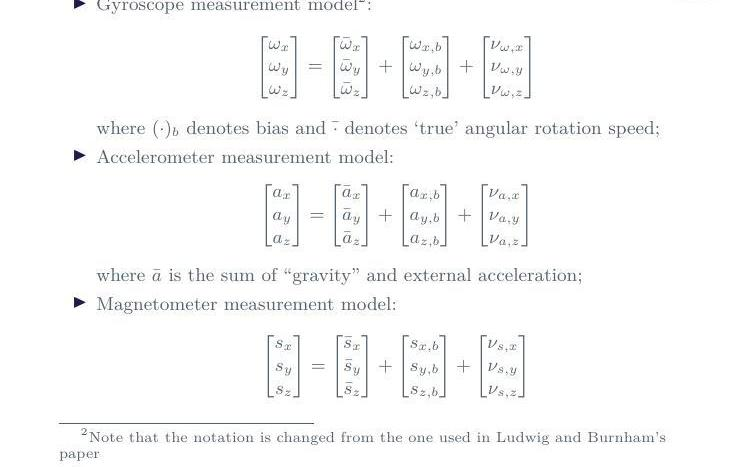
\includegraphics[width=\textwidth]{slide-21.jpg}
  \caption{Measurement models for all three IMU sensor types.
    Each sensor reading is the sum of three terms:
    the \textbf{true} physical quantity (tilde/bar notation),
    a \textbf{bias} (subscript $b$), and additive \textbf{noise} ($\nu$).
    The gyroscope measures angular rate; the accelerometer measures the sum
    of gravity and external acceleration; the magnetometer measures the
    ambient magnetic field.}
\end{figure}

All three IMU sensors share the same model structure:
\[
  \text{measured} = \text{true value} + \text{bias} + \text{noise}
\]

\textbf{Gyroscope} (angular rate, rad/s):
\[
  \begin{bmatrix} \omega_x \\ \omega_y \\ \omega_z \end{bmatrix}
  =
  \underbrace{\begin{bmatrix} \tilde{\omega}_x \\ \tilde{\omega}_y \\ \tilde{\omega}_z \end{bmatrix}}_{\text{true rate}}
  +
  \underbrace{\begin{bmatrix} \omega_{x,b} \\ \omega_{y,b} \\ \omega_{z,b} \end{bmatrix}}_{\text{bias}}
  +
  \underbrace{\begin{bmatrix} \nu_{\omega,x} \\ \nu_{\omega,y} \\ \nu_{\omega,z} \end{bmatrix}}_{\text{noise}}
\]

\textbf{Accelerometer} (specific force, m/s$^2$):
\[
  \begin{bmatrix} a_x \\ a_y \\ a_z \end{bmatrix}
  =
  \underbrace{\begin{bmatrix} \bar{a}_x \\ \bar{a}_y \\ \bar{a}_z \end{bmatrix}}_{\text{true specific force}}
  +
  \underbrace{\begin{bmatrix} a_{x,b} \\ a_{y,b} \\ a_{z,b} \end{bmatrix}}_{\text{bias}}
  +
  \underbrace{\begin{bmatrix} \nu_{a,x} \\ \nu_{a,y} \\ \nu_{a,z} \end{bmatrix}}_{\text{noise}}
\]

\textbf{Magnetometer} (magnetic field, $\mu$T):
\[
  \begin{bmatrix} s_x \\ s_y \\ s_z \end{bmatrix}
  =
  \underbrace{\begin{bmatrix} \bar{s}_x \\ \bar{s}_y \\ \bar{s}_z \end{bmatrix}}_{\text{true field}}
  +
  \underbrace{\begin{bmatrix} s_{x,b} \\ s_{y,b} \\ s_{z,b} \end{bmatrix}}_{\text{bias}}
  +
  \underbrace{\begin{bmatrix} \nu_{s,x} \\ \nu_{s,y} \\ \nu_{s,z} \end{bmatrix}}_{\text{noise}}
\]

\begin{center}
\begin{tabular}{@{} l p{3.0cm} p{7.4cm} @{}}
  \toprule
  Symbol & Name & Meaning \\
  \midrule
  $\tilde{\omega}$ & True angular rate &
    The real rotation rate of the body.
    Tilde $\tilde{\cdot}$ denotes the true unknown value. \\[3pt]
  $\omega_b$ & Gyroscope bias &
    A slowly drifting offset --- the gyroscope outputs a small nonzero
    value even when perfectly still.
    The main cause of orientation drift over time. \\[3pt]
  $\nu_\omega$ & Gyroscope noise &
    Fast zero-mean random noise.
    Modelled as Gaussian white noise. \\[3pt]
  $\bar{a}$ & True specific force &
    The true vector sum of gravity and any external linear acceleration.
    Bar $\bar{\cdot}$ denotes the true (noise- and bias-free) value.
    In steady state: $\bar{a} = (0,0,-g)^\top$ (NED). \\[3pt]
  $a_b$ & Accelerometer bias &
    Constant or slowly varying measurement offset. \\[3pt]
  $\bar{s}$ & True magnetic field &
    The true ambient magnetic field vector in the body frame. \\[3pt]
  $s_b$ & Magnetometer bias &
    Hard-iron and soft-iron distortion --- offsets caused by permanent
    magnets and ferromagnetic material near the sensor. \\
  \bottomrule
\end{tabular}
\end{center}

\begin{notebox}
  \textbf{Bias vs noise --- why bias is the bigger problem}

  Both corrupt the reading, but cause very different errors:

  \begin{itemize}[leftmargin=1.2em, itemsep=3pt]
    \item \textbf{Noise} is zero-mean and fast-varying.
      When integrated over time, positive and negative errors partially
      cancel.
      The orientation error grows as $\sqrt{t}$ --- a random walk.

    \item \textbf{Bias} is a constant offset always in the same direction.
      When integrated, it accumulates monotonically: every second adds the
      same wrong increment.
      The orientation error grows as $t$ --- linearly.
      A gyroscope bias of just $0.1^\circ$/s produces $6^\circ$ of heading
      error after one minute and a full $360^\circ$ after one hour.
  \end{itemize}

  This is why the Madgwick and Mahoney filters explicitly estimate and
  subtract the gyroscope bias $\omega_b$ as part of their update.
  Correcting bias is the single most important step for long-term stability.
\end{notebox}

\begin{notebox}
  \textbf{What the accelerometer actually measures --- and why gravity is
  useful}

  The accelerometer reads the \textbf{specific force}: all non-gravitational
  forces per unit mass.
  A body sitting still on a table feels the table pushing up against
  gravity --- the accelerometer reads that upward contact force, not
  gravity directly.

  \textbf{In steady state} (hovering, stationary, slow movement):
  \[
    \bar{a} = \begin{bmatrix} 0 \\ 0 \\ -g \end{bmatrix}
    \quad \text{(NED frame, } g \approx 9.81\,\text{m/s}^2\text{)}
  \]
  Only gravity is present.
  The \emph{direction} of this gravity vector in the body frame directly
  reveals roll and pitch: tilt the body and the measured gravity direction
  tilts with it.

  \textbf{During manoeuvres}, linear acceleration adds to gravity and the
  reading is no longer a pure gravity reference.

  This is the key subtlety: we are not using the accelerometer to measure
  how much the drone is accelerating --- that is not the goal here at all.
  We are using it as a \textbf{gravity direction sensor}.
  In steady state, the only force it feels is gravity, so the direction of
  its reading tells us which way is ``down'' in the body frame, and from
  that we extract roll and pitch.

  But when the drone actually accelerates (thrusts sideways, brakes, tilts
  aggressively), a second force --- the linear acceleration --- adds on top
  of gravity.
  The combined vector no longer points straight down; it points in some
  mixed direction that is \emph{not} the true gravity direction.
  If the filter uses that corrupted direction as a gravity reference, it
  will think the body is tilted when it is not, and introduce a wrong
  attitude correction.

  So: trusted less during acceleration not because we don't want to
  measure acceleration --- but because the gravity direction we need
  for attitude correction is hidden inside a mixture of gravity and
  linear acceleration, and we can no longer separate them.
  A simple check: if $\|\bar{a}\| \neq g$, the body is accelerating and
  the accelerometer reading is a corrupted gravity reference.
\end{notebox}

% ------------------------------------------------------------------------------
\subsection*{5.2 \quad Quaternion Kinematic Equation}
% ------------------------------------------------------------------------------

\begin{figure}[H]
  \centering
  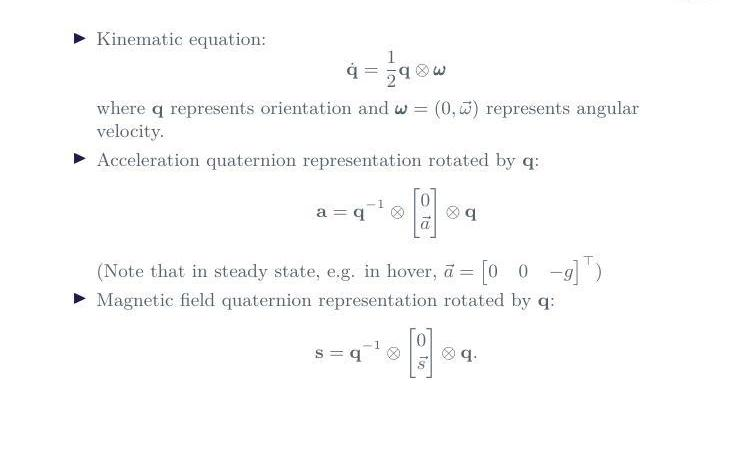
\includegraphics[width=\textwidth]{slide-22.jpg}
  \caption{Quaternion formulation of the IMU models.
    \textbf{Top}: the kinematic equation
    $\dot{\mathbf{q}} = \tfrac{1}{2}\mathbf{q}\otimes\boldsymbol{\omega}$
    shows how the orientation quaternion changes over time due to angular
    velocity.
    \textbf{Middle}: the world-frame gravity reference rotated into the body
    frame via $\mathbf{q}^{-1}(\cdot)\mathbf{q}$ gives the predicted
    accelerometer reading.
    \textbf{Bottom}: the same rotation applies to the magnetometer reference.}
\end{figure}

\textbf{The kinematic equation.}

As the body rotates, the orientation quaternion $\mathbf{q}$ changes over
time.
The rate of change is:
\[
  \boxed{\dot{\mathbf{q}} = \frac{1}{2}\,\mathbf{q} \otimes \boldsymbol{\omega}}
\]
where the angular velocity is embedded as a pure quaternion:
\[
  \boldsymbol{\omega}
  = \begin{bmatrix} 0 \\ \tilde{\omega}_x \\ \tilde{\omega}_y \\ \tilde{\omega}_z \end{bmatrix}
\]

\begin{center}
\begin{tabular}{@{} l p{3.0cm} p{7.4cm} @{}}
  \toprule
  Symbol & Name & Meaning \\
  \midrule
  $\dot{\mathbf{q}}$ & Quaternion derivative &
    Rate of change of all four quaternion components simultaneously. \\[3pt]
  $\boldsymbol{\omega}$ & Angular velocity (pure quaternion) &
    Gyroscope reading embedded with zero scalar part.
    In practice the bias-corrected rate:
    $(0,\;\omega_x - \omega_{x,b},\;\omega_y - \omega_{y,b},\;
    \omega_z - \omega_{z,b})$. \\[3pt]
  $\tfrac{1}{2}$ & Half-angle factor &
    Comes from the $\alpha/2$ in the quaternion definition.
    A physical rotation rate of $\dot{\alpha}$ rad/s corresponds to a
    quaternion rate of $\tfrac{1}{2}\dot{\alpha}$. \\
  \bottomrule
\end{tabular}
\end{center}

\begin{notebox}
  \textbf{Where the $\tfrac{1}{2}$ comes from}

  The quaternion stores $\cos(\alpha/2)$ and $\sin(\alpha/2)$, not $\alpha$
  directly.
  If the body rotates at rate $\dot{\alpha}$, then $\alpha/2$ changes at
  rate $\dot{\alpha}/2$.
  Differentiating $q_0 = \cos(\alpha/2)$:
  \[
    \dot{q}_0 = -\sin\!\tfrac{\alpha}{2}\cdot\tfrac{\dot{\alpha}}{2}
  \]
  The factor $\tfrac{1}{2}$ emerges from the chain rule and propagates
  through all four components, giving $\dot{\mathbf{q}} =
  \tfrac{1}{2}\mathbf{q}\otimes\boldsymbol{\omega}$.

  \textbf{Discrete integration} (Euler step with sample period $T_s$):
  \[
    \mathbf{q}_k
    = \mathbf{q}_{k-1} + \frac{T_s}{2}\,\mathbf{q}_{k-1}
      \otimes \boldsymbol{\omega}_{k-1}
    \quad\xrightarrow{\text{renormalise}}\quad
    \mathbf{q}_k \leftarrow \frac{\mathbf{q}_k}{\|\mathbf{q}_k\|}
  \]
  This is the \textbf{gyroscope integration step} --- it propagates
  orientation forward using only the gyroscope.
  No accelerometer or magnetometer is used here.
  Over time it drifts due to gyroscope bias; the Madgwick/Mahoney
  correction steps in Sections~6 and~7 counteract that drift.
\end{notebox}

\textbf{Reference vectors for correction.}

The accelerometer and magnetometer read in the \textbf{body frame}, but
their reference values (gravity, magnetic north) are known in the
\textbf{world frame}.
To compare prediction against measurement, rotate the world-frame reference
into the body frame using the inverse rotation $\mathbf{q}^{-1} =
\mathbf{q}^*$:

\[
  \mathbf{a}
  = \mathbf{q}^{-1} \otimes
    \begin{bmatrix} 0 \\ 0 \\ 0 \\ -g \end{bmatrix}
    \otimes \mathbf{q}
  \qquad\text{(in steady state)}
\]
\[
  \mathbf{s}
  = \mathbf{q}^{-1} \otimes
    \begin{bmatrix} 0 \\ \bar{s}_x \\ \bar{s}_y \\ \bar{s}_z \end{bmatrix}
    \otimes \mathbf{q}
\]

\begin{notebox}
  \textbf{What exactly is happening --- a concrete example}

  The filter holds a current orientation estimate $\mathbf{q}$.
  It uses $\mathbf{q}$ to \textbf{predict} what the accelerometer should
  read if that orientation is correct.
  It then compares that prediction to the \textbf{actual} sensor reading.
  Any mismatch means $\mathbf{q}$ is wrong and needs correcting.

  \textbf{Step 1 --- the world-frame reference.}
  Gravity in the world frame always points straight down:
  \[
    \bar{a}_\text{world}
    = \begin{bmatrix}0\\0\\0\\{-g}\end{bmatrix}
    \quad\text{(pure quaternion, NED: $z$ points down, specific force $= -g$)}
  \]
  This is fixed and known --- it never changes.

  \textbf{Step 2 --- rotate into the body frame.}
  The accelerometer sits on the body and reads forces in the body's own
  $x$/$y$/$z$ axes.
  To predict what it reads, take the world-frame gravity and rotate it
  into the body frame using $\mathbf{q}^{-1}(\cdot)\mathbf{q}$
  (world $\to$ body, the reverse of Section~4.5):
  \[
    \mathbf{a}_\text{predicted}
    = \mathbf{q}^{-1} \otimes \bar{a}_\text{world} \otimes \mathbf{q}
  \]

  \textbf{Concrete example --- drone rolled $90^\circ$ to the right.}
  The right wing is pointing straight down.
  In the body frame the $y$-axis (right) now aligns with world down.
  So gravity, which points down in the world, appears along the body
  $+y$ axis:
  \[
    \mathbf{a}_\text{predicted}
    = \begin{bmatrix}0\\0\\{-g}\\0\end{bmatrix}
    \;\to\;
    \vec{a}_\text{predicted} = (0,\,-g,\,0)^\top
  \]
  The filter therefore expects the accelerometer to read $(0, -g, 0)$
  in the body frame.

  \textbf{Step 3 --- compare to actual measurement.}
  \[
    \text{error} = \mathbf{a}_\text{predicted} - \mathbf{a}_\text{measured}
  \]
  If the orientation estimate $\mathbf{q}$ is exactly right, the predicted
  and measured body-frame vectors match and the error is zero.
  If $\mathbf{q}$ is slightly off, the error is nonzero and tells the
  filter which way to rotate $\mathbf{q}$ to reduce the mismatch.
  The same principle applies identically to the magnetometer with
  magnetic north as the world-frame reference instead of gravity.
\end{notebox}

% ── Key takeaways ─────────────────────────────────────────────────────────────
\begin{keybox}
  \textbf{Section 5 --- Key Takeaways}
  \begin{itemize}[leftmargin=1.2em, itemsep=2pt]
    \item All three IMU sensors follow:
      \textbf{measured = true + bias + noise}.
      Bias integrates into a linearly growing error ($\propto t$); noise
      grows as $\sqrt{t}$.
      Estimating and removing bias is the most critical step for long-term
      accuracy.

    \item In steady state the accelerometer reads gravity
      $\bar{a} = (0,0,-g)^\top$ (NED), giving a roll/pitch reference.
      The magnetometer gives a yaw reference.
      Both are unreliable during manoeuvres or near magnetic disturbances.

    \item The \textbf{kinematic equation}
      $\dot{\mathbf{q}} = \tfrac{1}{2}\mathbf{q}\otimes\boldsymbol{\omega}$
      propagates orientation from gyroscope data.
      Integrated: $\mathbf{q}_k = \mathbf{q}_{k-1} +
      \tfrac{T_s}{2}\mathbf{q}_{k-1}\otimes\boldsymbol{\omega}_{k-1}$,
      then renormalise.
      This step drifts without correction.

    \item World-frame references are rotated into the body frame via
      $\mathbf{q}^{-1}\otimes(\cdot)\otimes\mathbf{q}$ (inverse of Section
      4.5's body$\to$world rotation).
      The mismatch between predicted and measured body-frame vectors drives
      the correction in Sections~6 and~7.
  \end{itemize}
\end{keybox}

% ==============================================================================
\newpage
\section*{Section 6 \quad Madgwick Filter}
% ==============================================================================

The Madgwick filter is a computationally efficient attitude estimator
specifically designed for IMU data.
It is a \textbf{complementary filter operating on quaternions}: the gyroscope
drives the orientation forward (high-frequency path) and the accelerometer
and magnetometer correct it (low-frequency path) --- exactly the
complementary structure from Section~3, but applied to 3D orientation.
It also estimates and removes the gyroscope bias in real time.

% ------------------------------------------------------------------------------
\subsection*{6.1 \quad Algorithm Overview}
% ------------------------------------------------------------------------------

\begin{figure}[H]
  \centering
  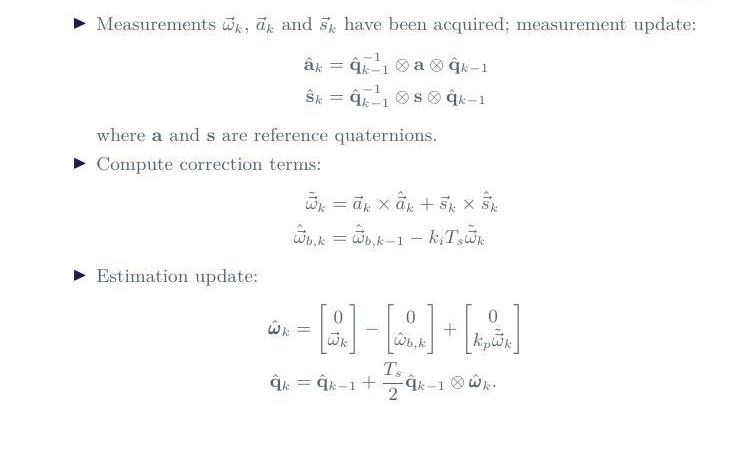
\includegraphics[width=\textwidth]{slide-23.jpg}
  \caption{Madgwick filter update equations.
    \textbf{Top}: predicted body-frame readings $\hat{a}_k$ and $\hat{s}_k$
    are computed by rotating the world-frame reference vectors into the body
    frame using the previous quaternion estimate $\hat{q}_{k-1}$.
    \textbf{Middle}: cross products between measured and predicted vectors
    give the correction direction $\tilde{\bar{\omega}}_k$; this is
    integrated to estimate the gyroscope bias $\tilde{\omega}_{b,k}$.
    \textbf{Bottom}: the bias-corrected and proportionally adjusted angular
    velocity drives the quaternion forward by one step.}
\end{figure}

The filter runs three steps every time step $k$:
\begin{enumerate}[leftmargin=1.6em, itemsep=4pt]
  \item \textbf{Predict} what the accelerometer and magnetometer should read
    given the current orientation estimate.
  \item \textbf{Compute the correction} from the mismatch between predicted
    and actual readings, and use it to update the gyroscope bias estimate.
  \item \textbf{Integrate} the corrected angular velocity to advance the
    quaternion.
\end{enumerate}

% ------------------------------------------------------------------------------
\subsection*{6.2 \quad Step 1 --- Predicted Body-Frame Readings}
% ------------------------------------------------------------------------------

Using the previous quaternion estimate $\hat{q}_{k-1}$, rotate the
world-frame reference vectors into the body frame (Section~5.2):
\[
  \hat{a}_k = \hat{q}_{k-1}^{-1} \otimes \mathbf{a} \otimes \hat{q}_{k-1},
  \qquad
  \hat{s}_k = \hat{q}_{k-1}^{-1} \otimes \mathbf{s} \otimes \hat{q}_{k-1}
\]
where $\mathbf{a} = (0,\,0,\,0,\,-g)$ is the world-frame gravity reference
and $\mathbf{s} = (0,\,\bar{s}_x,\,\bar{s}_y,\,\bar{s}_z)$ is the
world-frame magnetic field reference (both pure quaternions).

$\hat{a}_k$ is the \textbf{predicted accelerometer reading} in the body
frame --- what the sensor should read if $\hat{q}_{k-1}$ is correct.
$\hat{s}_k$ is the \textbf{predicted magnetometer reading}.

% ------------------------------------------------------------------------------
\subsection*{6.3 \quad Step 2 --- Correction Term and Bias Update}
% ------------------------------------------------------------------------------

The correction direction is found from the cross products between the
\emph{measured} (bias-corrected) and \emph{predicted} body-frame vectors:
\[
  \tilde{\bar{\omega}}_k
  = \tilde{a}_k \times \hat{a}_k
  + \tilde{s}_k \times \hat{s}_k
\]

\begin{notebox}
  \textbf{Why the cross product gives the correction direction}

  The cross product $\vec{u}\times\vec{v}$ produces a vector perpendicular
  to both $\vec{u}$ and $\vec{v}$, with magnitude
  $|\vec{u}||\vec{v}|\sin\phi$ where $\phi$ is the angle between them.

  \begin{itemize}[leftmargin=1.2em, itemsep=3pt]
    \item If the orientation estimate is \textbf{perfect}: $\tilde{a}_k$
      and $\hat{a}_k$ point in the same direction, $\phi = 0$, and
      $\tilde{a}_k\times\hat{a}_k = \vec{0}$ --- no correction needed.

    \item If the estimate is \textbf{slightly wrong}: the two vectors are
      misaligned by angle $\phi$.
      The cross product gives a vector pointing along the rotation axis
      about which the body frame must be rotated to bring them back into
      alignment, with magnitude $\approx \phi$ for small errors.
  \end{itemize}

  \textbf{Concrete example:}
  Suppose the drone is actually rolled $5^\circ$ right but the quaternion
  estimate thinks it is level.
  The predicted gravity $\hat{a}_k$ points straight down in the body frame
  (as if level), but the measured gravity $\tilde{a}_k$ is tilted $5^\circ$
  from down (because the body is actually tilted).
  The cross product $\tilde{a}_k\times\hat{a}_k$ points along the body
  $x$-axis (forward) and has magnitude $\sin 5^\circ \approx 0.087$.
  This tells the filter: ``rotate about $x$ to correct the roll by
  approximately $5^\circ$'' --- which is exactly the right correction.

  Adding both cross products means the accelerometer corrects roll and
  pitch (via gravity direction) and the magnetometer corrects yaw (via
  magnetic north direction).
  Together they constrain all three rotation axes.
\end{notebox}

The gyroscope \textbf{bias estimate} is updated by integrating the
correction:
\[
  \tilde{\omega}_{b,k}
  = \tilde{\omega}_{b,k-1} - k_I\, T_s\, \tilde{\bar{\omega}}_k
\]

\begin{center}
\begin{tabular}{@{} l p{2.8cm} p{7.6cm} @{}}
  \toprule
  Symbol & Name & Meaning \\
  \midrule
  $\tilde{\bar{\omega}}_k$ & Correction direction &
    Cross-product error signal telling the filter which way the orientation
    estimate needs to rotate. Zero when estimate is correct. \\[3pt]
  $\tilde{\omega}_{b,k}$ & Bias estimate &
    Current estimate of the gyroscope drift.
    Updated every step by integrating the correction signal. \\[3pt]
  $k_I$ & Integral gain &
    Controls how aggressively the bias estimate is updated.
    Large $k_I$: fast bias tracking but sensitive to disturbances.
    Small $k_I$: slow, smooth. \\[3pt]
  $T_s$ & Sample period & Time between filter updates (seconds). \\
  \bottomrule
\end{tabular}
\end{center}

\begin{notebox}
  \textbf{Why integrating the correction identifies the bias}

  If the gyroscope has a bias, the orientation estimate will be
  \emph{systematically} wrong in the same direction at every time step.
  The correction term $\tilde{\bar{\omega}}_k$ will therefore be
  persistently nonzero in the same direction.
  Integrating a persistent, directional signal builds up an estimate of
  that systematic offset --- which is exactly the bias.

  Once the bias estimate has converged to the true bias value, the
  subtraction in Step~3 cancels it and $\tilde{\bar{\omega}}_k$ drops
  to near zero.
  This is the \textbf{integral} action of the filter --- the same
  principle as the I-term in a PID controller eliminating steady-state
  error.
\end{notebox}

% ------------------------------------------------------------------------------
\subsection*{6.4 \quad Step 3 --- Corrected Angular Velocity and Quaternion
Update}
% ------------------------------------------------------------------------------

The corrected angular velocity combines three contributions:
\[
  \boldsymbol{\omega}_k
  = \underbrace{\begin{bmatrix} 0 \\ \tilde{\omega}_k \end{bmatrix}}_{\text{raw gyro}}
  - \underbrace{\begin{bmatrix} 0 \\ \tilde{\omega}_{b,k} \end{bmatrix}}_{\text{bias removal}}
  + \underbrace{\begin{bmatrix} 0 \\ k_P\,\tilde{\bar{\omega}}_k \end{bmatrix}}_{\text{proportional correction}}
\]

\begin{center}
\begin{tabular}{@{} l p{3.2cm} p{7.2cm} @{}}
  \toprule
  Term & Name & Meaning \\
  \midrule
  $\tilde{\omega}_k$ & Raw gyroscope rate &
    The bias-corrupted angular velocity from the gyroscope. \\[3pt]
  $-\tilde{\omega}_{b,k}$ & Bias removal &
    Subtract the current bias estimate to get the true angular rate.
    This is the bias correction discussed in Section~5. \\[3pt]
  $+k_P\tilde{\bar{\omega}}_k$ & Proportional correction &
    Add a fraction of the cross-product error to the angular velocity,
    giving an immediate push toward the correct orientation.
    $k_P$ controls how strongly the current mismatch corrects the estimate
    right now. \\
  \bottomrule
\end{tabular}
\end{center}

\begin{notebox}
  \textbf{The P and I gains --- PI controller on orientation error}

  \begin{itemize}[leftmargin=1.2em, itemsep=3pt]
    \item \textbf{$k_P$ (proportional)}: adds the current error
      $\tilde{\bar{\omega}}_k$ directly to the angular rate --- an
      immediate ``snap back'' toward the accelerometer/magnetometer
      reference.
      Large $k_P$ = fast correction but noisy, sensitive to vibration
      and magnetic disturbances.
      Small $k_P$ = smooth but slow to correct drift.

    \item \textbf{$k_I$ (integral)}: slowly accumulates the error to
      learn and cancel the gyroscope bias.
      Large $k_I$ = learns bias fast but can become unstable if the
      system is frequently disturbed.
      Small $k_I$ = stable, slow bias learning.
  \end{itemize}

  In practice $k_P \gg k_I$ --- the proportional correction acts on
  current error while the integral must be slow enough to distinguish
  true gyroscope drift from temporary accelerometer/magnetometer
  disturbances.
\end{notebox}


The quaternion is advanced by one step using the kinematic equation:
\[
  \hat{q}_k
  = \hat{q}_{k-1} + \frac{T_s}{2}\,\hat{q}_{k-1} \otimes \boldsymbol{\omega}_k
\]
followed by renormalisation:
$\hat{q}_k \leftarrow \hat{q}_k / \|\hat{q}_k\|$.

% ------------------------------------------------------------------------------
\subsection*{6.4b \quad Worked Example --- One Complete Filter Step}
% ------------------------------------------------------------------------------

\begin{notebox}
  \textbf{Scenario:} The filter's current estimate says the drone is
  perfectly level: $\hat{q}_{k-1} = (1,0,0,0)$.
  In reality, the drone has drifted to $10^\circ$ rolled to the right
  (about the body $x$-axis), but the filter does not know this yet.
  The gyroscope reads zero (no current rotation happening).
  No bias has been estimated yet: $\tilde{\omega}_{b,k-1} = (0,0,0)$.

  Parameters: $k_P = 2.0$,\; $k_I = 0.005$,\; $T_s = 0.01$\,s.

  \medskip
  \textbf{Step 1 --- Predicted body-frame readings.}

  Since $\hat{q}_{k-1}$ is the identity, rotating any world-frame vector
  into the body frame leaves it unchanged:
  \[
    \hat{a}_k
    = \hat{q}_{k-1}^{-1}\otimes(0,0,0,-1)\otimes\hat{q}_{k-1}
    = \begin{bmatrix}0\\0\\-1\end{bmatrix}
  \]
  (gravity normalised to 1, pointing in $-z$ body direction --- the filter
  believes the drone is level so gravity should be straight down.)

  \textbf{Step 2 --- Actual accelerometer reading.}

  The drone is actually rolled $10^\circ$ right.
  Gravity in the body frame now has a component along body $+y$
  (the right side is tilted down):
  \[
    \tilde{a}_k
    = \begin{bmatrix} 0 \\ \sin 10^\circ \\ -\cos 10^\circ \end{bmatrix}
    = \begin{bmatrix} 0 \\ 0.174 \\ -0.985 \end{bmatrix}
  \]

  \textbf{Step 3 --- Correction direction via cross product.}

  \[
    \tilde{\bar{\omega}}_k
    = \tilde{a}_k \times \hat{a}_k
    = \begin{bmatrix}0\\0.174\\-0.985\end{bmatrix}
      \times
      \begin{bmatrix}0\\0\\-1\end{bmatrix}
  \]
  \[
    = \begin{bmatrix}
        0.174\cdot(-1) - (-0.985)\cdot 0 \\
        (-0.985)\cdot 0 - 0\cdot(-1) \\
        0\cdot 0 - 0.174\cdot 0
      \end{bmatrix}
    = \begin{bmatrix}-0.174\\0\\0\end{bmatrix}
  \]
  The correction points in the $-x$ direction.
  \textbf{Reading this:} the filter needs to rotate the estimate about
  the $-x$ axis (roll left) by approximately $\sin^{-1}(0.174) = 10^\circ$
  --- which is exactly right, since the estimate is $10^\circ$ too far
  right.

  \textbf{Step 4 --- Bias update.}
  \[
    \tilde{\omega}_{b,k}
    = (0,0,0) - 0.005\times 0.01\times (-0.174,0,0)
    = (0.0000087,\;0,\;0)\;\text{rad/s}
  \]
  After just one step the bias estimate is tiny --- the integral builds
  up slowly over many steps.
  If the $10^\circ$ roll error persists (e.g.\ because of a real gyroscope
  bias), the correction $(-0.174, 0, 0)$ will be nonzero at every step,
  and the integral will accumulate into a meaningful bias estimate over
  time.

  \textbf{Step 5 --- Corrected angular velocity.}
  \[
    \boldsymbol{\omega}_k
    = \underbrace{(0,0,0)}_{\text{gyro}}
    - \underbrace{(0.0000087,0,0)}_{\text{bias}}
    + \underbrace{2.0\times(-0.174,0,0)}_{k_P\,\tilde{\bar{\omega}}_k}
    = (-0.348,\;0,\;0)\;\text{rad/s}
  \]
  The dominant term is the proportional correction: $-0.348$ rad/s about
  the $x$-axis.
  This makes the filter behave as if the drone is currently rolling
  \emph{left} at $0.348$ rad/s --- pushing the estimate back toward the
  true orientation.

  \textbf{Step 6 --- Quaternion update.}

  Embed $\boldsymbol{\omega}_k$ as a pure quaternion:
  $(0,\;-0.348,\;0,\;0)$.

  Since $\hat{q}_{k-1} = (1,0,0,0)$, the product
  $\hat{q}_{k-1}\otimes\boldsymbol{\omega}_k = (0,-0.348,0,0)$.
  \[
    \hat{q}_k
    = (1,0,0,0) + \frac{0.01}{2}(0,-0.348,0,0)
    = (1,\;-0.00174,\;0,\;0)
  \]
  After renormalisation: $\hat{q}_k \approx (1.000,\;-0.00174,\;0,\;0)$.

  \textbf{What this means:} $q_x = -0.00174 = \sin(\alpha/2)$ for a small
  negative rotation about $x$.
  This corresponds to a $\approx 0.2^\circ$ roll to the left applied to
  the estimate in this one step.
  Starting from $0^\circ$ error, after this step the estimate is $0.2^\circ$
  closer to the true $10^\circ$ roll.
  After $\approx 50$ steps ($0.5$ seconds) the estimate would catch up to
  the true orientation.

  \textbf{Summary of what changed in this one step:}

  \medskip
  \begin{tabular}{@{} l p{4.5cm} p{5.5cm} @{}}
    \toprule
    Quantity & Before & After \\
    \midrule
    Quaternion $\hat{q}$ &
      $(1,\;0,\;0,\;0)$ --- level &
      $(1,\;-0.00174,\;0,\;0)$ --- $0.2^\circ$ roll left
      (toward true orientation) \\[4pt]
    Bias estimate $\tilde{\omega}_{b}$ &
      $(0,\;0,\;0)$ &
      $(0.0000087,\;0,\;0)$ --- tiny start of integral \\[4pt]
    Cross product error &
      --- &
      $(-0.174,\;0,\;0)$ --- points $-x$, says ``roll left'' \\
    \bottomrule
  \end{tabular}
\end{notebox}
\begin{notebox}
  \textbf{$k_P$ does react to noise --- and $k_I$ is specifically why
  that does not ruin the bias estimate}

  You are right: $k_P$ multiplies the \emph{current} cross-product error
  $\tilde{\bar{\omega}}_k$, which contains \emph{both} real orientation
  error \emph{and} sensor noise.
  A noise spike in the accelerometer produces a nonzero cross product for
  that one step, and $k_P$ immediately pushes the quaternion in the wrong
  direction.
  This is an unavoidable cost of the proportional term --- it cannot tell
  the difference between ``the estimate is wrong'' and ``the sensor had
  a noise spike''.
  Keeping $k_P$ small reduces this sensitivity but also slows down
  genuine corrections.

  The integral term $k_I$ is more robust to noise because noise is
  \textbf{zero-mean}: a positive spike at one step is followed by a
  negative spike at the next.
  Integrating zero-mean noise over many steps, the positive and negative
  contributions cancel and the integral stays near zero.
  But a real gyroscope bias pushes the error in the \emph{same direction
  every single step} --- those never cancel.
  Integrating a persistent, one-directional signal builds up to a
  significant estimate; integrating zero-mean noise stays near zero.
  This is exactly why $k_I$ learns bias without being driven by noise.

  \textbf{Does this only work if the bias is a fixed offset?}

  No --- it also works when the bias changes, but with an important caveat
  about \emph{how fast} it changes:

  \begin{itemize}[leftmargin=1.2em, itemsep=3pt]
    \item \textbf{Fixed offset, different value every startup:} works
      perfectly.
      Every time the filter starts, it begins with zero bias estimate and
      converges to whatever the current bias is within a few seconds.
      Different startup, different bias value --- the integral finds it
      each time.

    \item \textbf{Slowly drifting bias} (e.g.\ temperature changes over
      minutes): still works.
      As the bias slowly drifts, the persistent correction signal shifts
      direction slowly, and the integral tracks it.
      As long as the bias changes \emph{much slower} than $k_I$ can
      integrate, the estimate follows it.

    \item \textbf{Rapidly changing bias} (changes fast compared to the
      integration speed $k_I$): the integral falls behind.
      The estimate always lags the true bias, causing residual drift.
      Increasing $k_I$ would help track faster changes but at the cost
      of being more sensitive to noise --- the fundamental trade-off.
  \end{itemize}

  In practice, gyroscope bias drifts on timescales of seconds to minutes
  (thermal drift, mechanical relaxation), so a slow $k_I$ is almost
  always fast enough to track it while still rejecting noise.
\end{notebox}

% ------------------------------------------------------------------------------
\subsection*{6.5 \quad Flight Experiment and Performance}
% ------------------------------------------------------------------------------

\begin{figure}[H]
  \centering
  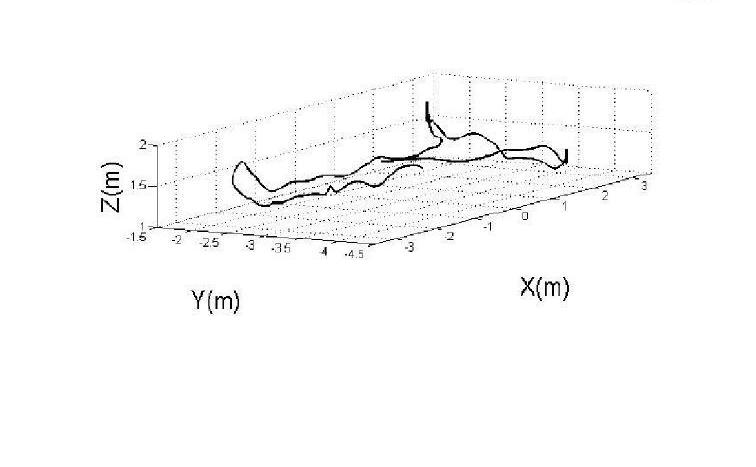
\includegraphics[width=0.8\textwidth]{slide-25.jpg}
  \caption{3D flight trajectory during the experiment.
    The drone flew over a volume of roughly $5\,\text{m}\times8\,\text{m}
    \times1\,\text{m}$.
    This trajectory was used to evaluate the attitude filters --- the IMU
    data recorded here was processed by the Madgwick, Mahoney, and EKF
    filters and compared against a ground-truth reference.}
\end{figure}

\begin{figure}[H]
  \centering
  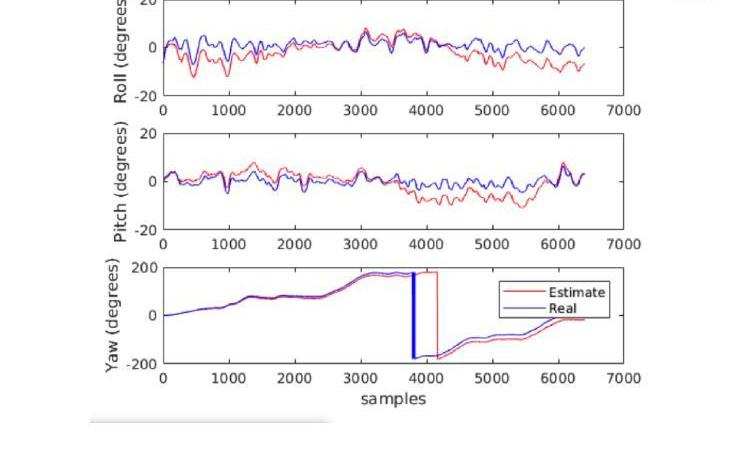
\includegraphics[width=0.8\textwidth]{slide-26.jpg}
  \caption{Madgwick filter performance.
    \textbf{Red}: filter estimate. \textbf{Blue}: ground truth.
    \textbf{Top}: roll $\phi$ --- tracked well throughout.
    \textbf{Middle}: pitch $\theta$ --- similarly accurate.
    \textbf{Bottom}: yaw $\psi$ --- larger errors, particularly around
    sample 3500--4000 where a rapid manoeuvre caused a temporary spike.
    Yaw is harder because it relies on the magnetometer, which is more
    susceptible to motor magnetic disturbance than the accelerometer used
    for roll and pitch.}
\end{figure}

\begin{notebox}
  \textbf{Why yaw is harder than roll and pitch}

  Roll and pitch are corrected by the \textbf{accelerometer} via gravity.
  Gravity is strong ($\approx 9.81$\,m/s$^2$), stable, and always present.

  Yaw is corrected by the \textbf{magnetometer} via magnetic north.
  The Earth's field is 10--60\,$\mu$T --- much weaker.
  A quadcopter's motors and speed controllers generate magnetic fields that
  can easily overwhelm the Earth's field near the sensor.
  When the motors change speed during aggressive manoeuvres, the local
  disturbance changes, causing spikes the filter misinterprets as yaw
  changes.
  This is visible in the bottom plot: roll and pitch track well
  throughout, but yaw spikes when the motors are stressed.
\end{notebox}

% ── Key takeaways ─────────────────────────────────────────────────────────────
\begin{keybox}
  \textbf{Section 6 --- Key Takeaways}
  \begin{itemize}[leftmargin=1.2em, itemsep=2pt]
    \item Madgwick is a quaternion complementary filter: gyroscope
      integration (fast path) + accelerometer/magnetometer correction
      (slow path) + gyroscope bias estimation.

    \item \textbf{Correction}: $\tilde{\bar{\omega}}_k =
      \tilde{a}_k\times\hat{a}_k + \tilde{s}_k\times\hat{s}_k$.
      Cross product = zero when estimate is correct; nonzero mismatch
      gives the rotation axis and approximate angle of error.

    \item \textbf{Bias update}: $\tilde{\omega}_{b,k} =
      \tilde{\omega}_{b,k-1} - k_I T_s\tilde{\bar{\omega}}_k$.
      Persistent nonzero correction identifies and cancels gyroscope drift.

    \item \textbf{Quaternion update}: $\hat{q}_k = \hat{q}_{k-1} +
      \tfrac{T_s}{2}\hat{q}_{k-1}\otimes\boldsymbol{\omega}_k$, with
      $\boldsymbol{\omega}_k$ = raw gyro $-$ bias $+$ $k_P$ correction.
      Renormalise after every step.

    \item $k_P \gg k_I$ in practice: proportional corrects now, integral
      slowly learns bias.

    \item Yaw harder than roll/pitch: gravity reference (accel) is strong
      and stable; magnetic north (mag) is weak and disturbed by motors.
  \end{itemize}
\end{keybox}

% ==============================================================================
\newpage
\section*{Section 7 \quad Mahoney Filter \& Performance Comparison}
% ==============================================================================

The Mahoney filter solves exactly the same problem as Madgwick --- quaternion
attitude estimation from gyroscope, accelerometer and magnetometer --- but
uses a slightly different mathematical approach to find the correction
direction.
Instead of the cross product, it computes a \textbf{Jacobian-based gradient
descent}: the direction in quaternion space that most steeply reduces the
total sensor error.
The structure is otherwise identical: gyroscope integration corrected by
accelerometer and magnetometer, with bias estimation.

% ------------------------------------------------------------------------------
\subsection*{7.1 \quad Magnetometer Pre-Processing}
% ------------------------------------------------------------------------------

\begin{figure}[H]
  \centering
  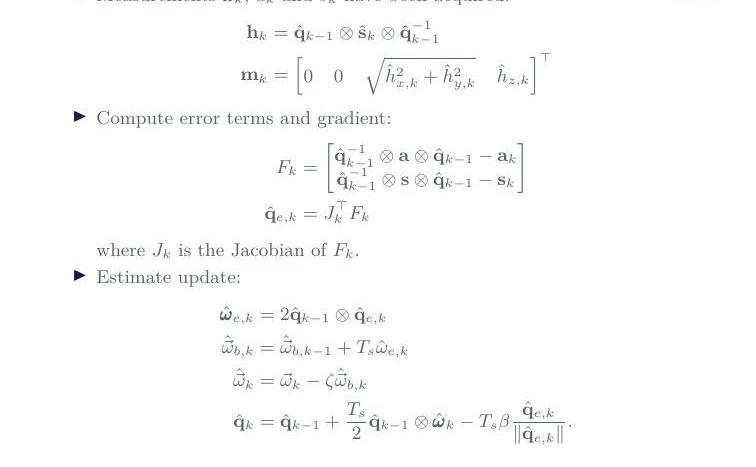
\includegraphics[width=\textwidth]{slide-24.jpg}
  \caption{Mahoney filter update equations.
    \textbf{Top}: the magnetometer reading is rotated to the world frame
    ($\mathbf{h}_k$) then projected onto the horizontal plane
    ($\mathbf{m}_k$) to decouple yaw correction from roll/pitch.
    \textbf{Middle}: $F_k$ stacks the accelerometer and magnetometer
    prediction errors; the Jacobian $J_k$ maps this into quaternion space
    as the gradient $\hat{q}_{e,k}$.
    \textbf{Bottom}: the gradient drives both the quaternion update and the
    bias estimate.}
\end{figure}

Before computing the correction, the Mahoney filter pre-processes the
magnetometer reading to separate the yaw information from roll/pitch.

\textbf{Rotate the measured field to the world frame:}
\[
  \mathbf{h}_k
  = \hat{q}_{k-1} \otimes \tilde{s}_k \otimes \hat{q}_{k-1}^{-1}
\]
$\mathbf{h}_k = (0, h_x, h_y, h_z)$ is the estimated world-frame magnetic
field.

\textbf{Project onto the horizontal plane:}
\[
  \mathbf{m}_k
  = \begin{bmatrix} 0 \\[2pt]
      \sqrt{h_{x,k}^2 + h_{y,k}^2} \\[2pt] 0 \\[2pt] h_{z,k}
    \end{bmatrix}
\]

\begin{notebox}
  \textbf{Why project onto the horizontal plane?}

  Only the \textbf{horizontal component} of the Earth's field points
  toward magnetic north and carries yaw information.
  The vertical component is the same regardless of which way you face ---
  it tells you nothing about yaw.

  The problem: when the drone is rolled or pitched, the body-frame
  magnetometer reading mixes horizontal and vertical components together.
  A $5^\circ$ roll error bleeds some vertical field into the horizontal
  reading and vice versa --- the raw body-frame reading is a corrupted yaw
  reference.

  By first rotating the reading to the world frame ($\mathbf{h}_k$)
  and keeping only the horizontal magnitude
  $\sqrt{h_x^2 + h_y^2}$ and vertical $h_z$, the filter reconstructs a
  reference $\mathbf{m}_k$ that is \textbf{always horizontal} regardless
  of any roll or pitch.
  Yaw and roll/pitch corrections are then independent of each other.
\end{notebox}

% ------------------------------------------------------------------------------
\subsection*{7.2 \quad Error, Gradient and Update Equations}
% ------------------------------------------------------------------------------

\textbf{Error function.}
Stack the prediction errors for both sensors:
\[
  F_k =
  \begin{bmatrix}
    \hat{q}_{k-1}^{-1} \otimes \mathbf{a} \otimes \hat{q}_{k-1}
    - \tilde{a}_k \\[4pt]
    \hat{q}_{k-1}^{-1} \otimes \mathbf{m}_k \otimes \hat{q}_{k-1}
    - \tilde{s}_k
  \end{bmatrix}
\]
$F_k = \mathbf{0}$ when the orientation estimate is perfect.

\textbf{Gradient in quaternion space:}
\[
  \hat{q}_{e,k} = J_k^\top F_k
\]
where $J_k$ is the Jacobian of $F_k$ with respect to the quaternion
components.
$\hat{q}_{e,k}$ is a 4-vector pointing in the direction of steepest error
increase in quaternion space --- the filter steps in the opposite direction.

\begin{notebox}
  \textbf{Cross product (Madgwick) vs Jacobian gradient (Mahoney)}

  Both find a correction direction from the same sensor mismatch:

  \begin{itemize}[leftmargin=1.2em, itemsep=3pt]
    \item \textbf{Madgwick}: $\tilde{a}_k \times \hat{a}_k$ --- geometric
      axis perpendicular to the two vectors, magnitude $\approx \sin\phi$.
      Fast, no Jacobian needed, but only uses vector geometry.

    \item \textbf{Mahoney}: $J_k^\top F_k$ --- mathematically the direction
      of steepest descent in the full 4D quaternion space.
      More principled, accounts for how each quaternion component
      contributes to each sensor output.
  \end{itemize}

  For small errors both give nearly the same correction --- which is why
  their performance on the flight data is similar.
  The Mahoney gradient is theoretically more exact; the Madgwick cross
  product is a fast geometric approximation.
\end{notebox}

\textbf{Update equations.}

Convert the quaternion gradient to an angular velocity correction:
\[
  \tilde{\omega}_{e,k} = 2\,\hat{q}_{k-1} \otimes \hat{q}_{e,k}
\]

Update bias estimate:
\[
  \tilde{\omega}_{b,k} = \tilde{\omega}_{b,k-1} + T_s\,\tilde{\omega}_{e,k}
\]

Apply bias correction to gyroscope:
\[
  \tilde{\omega}_k \leftarrow \tilde{\omega}_k - \zeta\,\tilde{\omega}_{b,k}
\]

Update quaternion:
\[
  \hat{q}_k
  = \hat{q}_{k-1}
  + \frac{T_s}{2}\,\hat{q}_{k-1} \otimes \tilde{\omega}_k
  - T_s\,\beta\,\frac{\hat{q}_{e,k}}{\|\hat{q}_{e,k}\|}
\]

\begin{center}
\begin{tabular}{@{} l p{3.0cm} p{7.4cm} @{}}
  \toprule
  Symbol & Name & Meaning \\
  \midrule
  $\hat{q}_{e,k}$ & Quaternion gradient &
    Steepest ascent direction in quaternion space.
    Filter steps against it. \\[3pt]
  $\tilde{\omega}_{e,k}$ & Angular correction &
    Gradient converted to equivalent angular velocity for bias update. \\[3pt]
  $\beta$ & Gradient gain &
    Controls how strongly the normalised gradient corrects the quaternion.
    Equivalent to $k_P$ in Madgwick. \\[3pt]
  $\zeta$ & Bias gain &
    Controls how strongly the bias estimate is applied.
    Equivalent to $k_I$ in Madgwick. \\[3pt]
  $\hat{q}_{e,k}/\|\hat{q}_{e,k}\|$ & Normalised gradient &
    The gradient is normalised before applying: step size is fixed at
    $\beta T_s$ regardless of error magnitude.
    Madgwick's cross product is \emph{not} normalised --- larger errors
    give larger automatic corrections. \\
  \bottomrule
\end{tabular}
\end{center}

% ------------------------------------------------------------------------------
\subsection*{7.2b \quad Worked Example --- One Complete Mahoney Step}
% ------------------------------------------------------------------------------

\begin{notebox}
  \textbf{Same scenario as the Madgwick example:}
  $\hat{q}_{k-1} = (1,0,0,0)$, drone drifted $10^\circ$ rolled right,
  gyroscope reads zero, zero initial bias.
  Parameters: $\beta = 2.0$,\; $\zeta = 0.005$,\; $T_s = 0.01$\,s.

  \medskip
  \textbf{Step 1 --- Magnetometer pre-processing.}

  Suppose the magnetometer reads
  $\tilde{s}_k = (0.7, 0.5, 0.3)$ (body frame, after bias removal,
  normalised for simplicity) and the reference world-frame magnetic field
  is known as $\bar{s} = (1, 0, 0.3)$ (pointing mostly North with a
  vertical dip component).

  Rotate measured field to world frame:
  \[
    \mathbf{h}_k
    = \hat{q}_{k-1} \otimes \tilde{s}_k \otimes \hat{q}_{k-1}^{-1}
  \]
  At identity, this leaves $\tilde{s}_k$ unchanged:
  $\mathbf{h}_k = (0,\; 0.7,\; 0.5,\; 0.3)$.

  Project onto horizontal plane (keep horizontal magnitude and vertical
  component, zero out the other horizontal component):
  \[
    \mathbf{m}_k
    = \begin{bmatrix}0 \\ \sqrt{0.7^2+0.5^2} \\ 0 \\ 0.3\end{bmatrix}
    = \begin{bmatrix}0 \\ 0.860 \\ 0 \\ 0.3\end{bmatrix}
  \]
  This is now the reference used for yaw correction --- it is always
  horizontal regardless of any roll or pitch in the estimate.

  \medskip
  \textbf{Step 2 --- Predicted body-frame readings (same as Madgwick).}

  At identity: $\hat{a}_k = (0, 0, -1)$ (gravity straight down in body).

  \medskip
  \textbf{Step 3 --- Error function $F_k$.}

  Using the same accelerometer reading as the Madgwick example:
  $\tilde{a}_k = (0,\, 0.174,\, -0.985)$.
  \[
    F_{acc} = \hat{a}_k - \tilde{a}_k
    = (0,0,-1) - (0,0.174,-0.985)
    = (0,\; -0.174,\; -0.015)
  \]
  (For the magnetometer part we skip the computation for brevity;
  the accelerometer already captures the main roll correction.)

  \medskip
  \textbf{Step 4 --- Jacobian $J_k$ at the identity quaternion.}

  For the accelerometer function
  $f_{acc}(\mathbf{q}) = \hat{q}^{-1}\otimes(0,0,0,-1)\otimes\hat{q}$,
  the Jacobian evaluated at $\hat{q} = (1,0,0,0)$ is:
  \[
    J_{acc}
    = \frac{\partial f_{acc}}{\partial (q_0,q_x,q_y,q_z)}
      \bigg|_{(1,0,0,0)}
    = \begin{bmatrix}
        0  & 0  &  2 & 0 \\
        0  & -2 &  0 & 0 \\
        -2 & 0  &  0 & 0
      \end{bmatrix}
  \]
  Each column is how a small nudge in that quaternion component changes
  the predicted gravity vector.
  Column $q_x$ ($\partial f/\partial q_x = (0,-2,0)$) says: a small
  positive roll pushes the predicted $y$-component of gravity downward
  (more negative).

  \medskip
  \textbf{Step 5 --- Gradient $\hat{q}_{e,k} = J_k^\top F_k$.}
  \[
    J_{acc}^\top =
    \begin{bmatrix}
       0 &  0 & -2 \\
       0 & -2 &  0 \\
       2 &  0 &  0 \\
       0 &  0 &  0
    \end{bmatrix}, \qquad
    F_{acc} = \begin{bmatrix}0\\-0.174\\-0.015\end{bmatrix}
  \]
  \[
    \hat{q}_{e} = J_{acc}^\top F_{acc}
    = \begin{bmatrix}
        0(0)+0(-0.174)+(-2)(-0.015) \\
        0(0)+(-2)(-0.174)+0(-0.015) \\
        2(0)+0(-0.174)+0(-0.015) \\
        0
      \end{bmatrix}
    = \begin{bmatrix}0.03\\0.348\\0\\0\end{bmatrix}
    \approx
    \begin{bmatrix}0\\0.348\\0\\0\end{bmatrix}
  \]
  The gradient points in the $+q_x$ direction --- the same correction
  axis as the Madgwick cross product.

  \medskip
  \textbf{Step 6 --- Normalise and apply the gradient.}
  \[
    \|\hat{q}_e\| \approx 0.348, \qquad
    \frac{\hat{q}_e}{\|\hat{q}_e\|} \approx (0,\;1,\;0,\;0)
  \]
  \[
    \text{Gradient correction step}
    = -T_s \beta \frac{\hat{q}_e}{\|\hat{q}_e\|}
    = -0.01 \times 2.0 \times (0,1,0,0)
    = (0,\;-0.02,\;0,\;0)
  \]

  \textbf{Step 7 --- Bias update.}
  \[
    \tilde{\omega}_{e} = 2\hat{q}_{k-1}\otimes\hat{q}_e
    = 2(1,0,0,0)\otimes(0,0.348,0,0)
    = (0,\;0.696,\;0,\;0)
  \]
  \[
    \tilde{\omega}_{b} = (0,0,0) + T_s\tilde{\omega}_e
    = 0.01\times(0,0.696,0,0)
    = (0,\;0.00696,\;0,\;0)
  \]
  Apply bias: $\tilde{\omega}_k \leftarrow (0,0,0) - \zeta\tilde{\omega}_b
  = -0.005\times(0,0.00696,0,0) \approx (0,0,0)$ (negligible this step).

  \textbf{Step 8 --- Quaternion update.}
  \[
    \hat{q}_k
    = \underbrace{(1,0,0,0)}_{\hat{q}_{k-1}}
    + \underbrace{0}_{\text{gyro term (gyro=0)}}
    + \underbrace{(0,-0.02,0,0)}_{\text{gradient step}}
    = (1,\;-0.02,\;0,\;0)
  \]
  After renormalisation: $\hat{q}_k \approx (0.9998,\;-0.02,\;0,\;0)$.

  \medskip
  \textbf{Comparing Madgwick and Mahoney on the same step:}

  \medskip
  \begin{tabular}{@{} l l l l @{}}
    \toprule
    & \textbf{Madgwick} & \textbf{Mahoney} & \textbf{Same direction?}\\
    \midrule
    Correction method & Cross product $\tilde{a}\times\hat{a}$ &
      Jacobian $J^TF$ & Yes \\
    Correction direction & $(-0.174, 0, 0)$ angular rate &
      $(0, -0.02, 0, 0)$ quaternion & Yes (both $-q_x$)\\
    $q_x$ after update & $+0.00174$ & $-0.02$ & Same sign \\
    Correction size/step & $\propto \sin\phi$ (scales with error) &
      $= \beta T_s = 0.02$ (fixed) & Different \\
    \bottomrule
  \end{tabular}

  \medskip
  Both methods move the quaternion in the same direction.
  The key difference is the \textbf{normalisation}: Mahoney always
  takes a step of size $\beta T_s = 0.02$ regardless of how large the
  error is; Madgwick takes a step proportional to $\sin\phi \approx 0.174$,
  so small errors produce small corrections automatically.
\end{notebox}

% ------------------------------------------------------------------------------
\subsection*{7.3 \quad Performance and Comparison with EKF}
% ------------------------------------------------------------------------------

\begin{figure}[H]
  \centering
  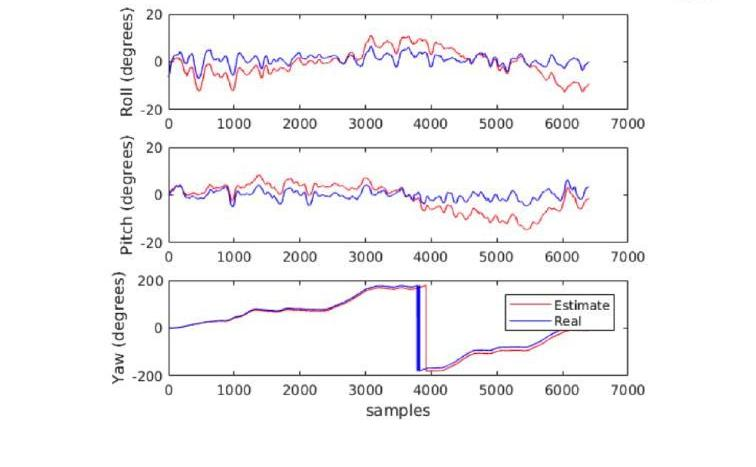
\includegraphics[width=\textwidth]{slide-27.jpg}
  \caption{Mahoney filter performance.
    \textbf{Red}: filter estimate. \textbf{Blue}: ground truth.
    Roll and pitch are well tracked throughout.
    Yaw shows the same spike at sample 3500--4000 as Madgwick (same
    magnetometer disturbance, same cause).
    Outside the spike, Mahoney's general yaw tracking is slightly cleaner
    than Madgwick's --- a direct benefit of the horizontal plane
    projection in Section~7.1, which prevents roll/pitch estimation errors
    from bleeding into the yaw correction.
    Madgwick uses the raw body-frame magnetometer reading, so any small
    tilt error in the estimate contaminates the yaw correction;
    Mahoney's projection decouples them.}
\end{figure}

\begin{warnbox}
  \textbf{The yaw problem is a sensor issue, not a filter issue}

  Madgwick, Mahoney, and the EKF below all show the same yaw spike at the
  same moment.
  This is because all three rely on the \textbf{magnetometer} for yaw
  correction, and the magnetometer is disturbed at that moment by the
  drone's own motors.

  Roll and pitch use \textbf{gravity} as a reference --- strong
  ($9.81\,\text{m/s}^2$), constant, unaffected by electronics or
  manoeuvres.
  Yaw uses the \textbf{Earth's magnetic field} --- weak
  ($\sim$50\,$\mu$T), easily overwhelmed by motor and ESC currents which
  change every time the drone manoeuvres.

  Changing the filter algorithm does not help because the information
  was never in the sensor reading to begin with.
  The fix is hardware: mount the magnetometer far from the motors, or use
  a different yaw reference entirely (GPS heading, optical flow, external
  tracking system).
\end{warnbox}

\begin{figure}[H]
  \centering
  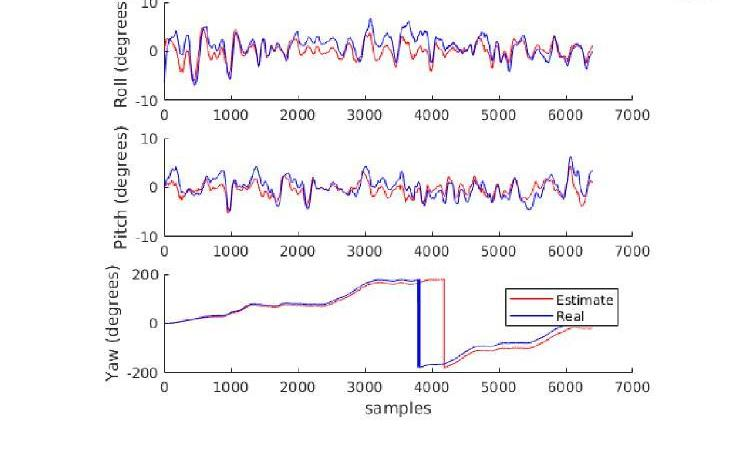
\includegraphics[width=\textwidth]{slide-28.jpg}
  \caption{Extended Kalman Filter performance on the same flight data.
    Roll and pitch are tracked more accurately than both Madgwick and
    Mahoney.
    Yaw still spikes at the same location --- confirming this is a
    magnetometer disturbance that no filter algorithm can overcome.
    The EKF achieves better accuracy at significantly higher
    computational cost.}
\end{figure}

\begin{notebox}
  \textbf{Madgwick vs Mahoney vs EKF --- when to use which}

  \medskip
  \begin{tabular}{@{} p{2.4cm} p{3.2cm} p{3.2cm} p{3.0cm} @{}}
    \toprule
    & \textbf{Madgwick} & \textbf{Mahoney} & \textbf{EKF} \\
    \midrule
    Correction method &
      Cross product &
      Jacobian gradient &
      Kalman gain (optimal) \\[4pt]
    Noise model &
      None --- hand-tuned $k_P$, $k_I$ &
      None --- hand-tuned $\beta$, $\zeta$ &
      Explicit $Q$, $R$ covariances \\[4pt]
    CPU cost &
      Very low &
      Low &
      High \\[4pt]
    Roll/pitch &
      Good &
      Good &
      Best \\[4pt]
    Yaw &
      \multicolumn{3}{c}{Limited by magnetometer --- same for all three} \\[4pt]
    Best for &
      Microcontrollers, drones &
      Same &
      High-accuracy systems \\
    \bottomrule
  \end{tabular}

  \medskip
  All three share the same fundamental structure.
  The EKF is statistically optimal given a correct noise model;
  Madgwick and Mahoney replace the noise model with tunable gains,
  which is simpler and cheaper but less principled.
  For most embedded drone applications Madgwick or Mahoney is the
  practical choice.
\end{notebox}

% ── Key takeaways ─────────────────────────────────────────────────────────────
\begin{keybox}
  \textbf{Section 7 --- Key Takeaways}
  \begin{itemize}[leftmargin=1.2em, itemsep=2pt]
    \item Mahoney uses \textbf{Jacobian gradient descent}
      $\hat{q}_{e,k} = J_k^\top F_k$ rather than cross product.
      Similar performance in practice; more principled mathematically.

    \item The magnetometer is \textbf{projected onto the horizontal plane}
      ($\mathbf{m}_k$) to decouple yaw correction from roll/pitch.
      Prevents tilt errors from contaminating the yaw estimate.

    \item Gains: $\beta$ = gradient correction strength (like $k_P$);
      $\zeta$ = bias learning rate (like $k_I$).
      Gradient is \textbf{normalised} before applying --- fixed step size
      unlike Madgwick's unnormalised cross product.

    \item \textbf{The yaw spike is identical in all three filters.}
      It is a magnetometer hardware problem, not a filter design problem.
      No algorithm can recover information the sensor never contained.

    \item Choose Madgwick/Mahoney for embedded low-CPU use with
      hand-tuned gains; choose EKF when accuracy is critical and a
      noise model is available.
  \end{itemize}
\end{keybox}

% ==============================================================================
\newpage
\section*{Lecture Summary --- Sensor Fusion from Kalman to Attitude Filters}
% ==============================================================================

This lecture developed sensor fusion from its most general form down to
three specific algorithms, each making progressively more specialised
assumptions.
Here is the connecting thread.

% ------------------------------------------------------------------------------
\begin{keybox}
  \textbf{1 --- Kalman Filter for Multi-Sensor Fusion (Section 2)}

  The most general approach.
  The challenge is that multiple sensors can have \textbf{correlated noise}
  between them --- if two sensors share a power supply, a common clock, or
  the same environmental disturbance, their errors are not independent.
  Directly applying the standard KF ignores this and produces an
  overconfident, suboptimal estimate.

  The fix is the \textbf{Cholesky decorrelation}: factorise
  $R_k = L_k^\top L_k$, then transform all measurements by
  $T_k = (L_k^{-1})^\top$.
  This produces transformed channels with identity covariance
  $\bar{R}_k = I$ --- fully independent, unit variance.
  The standard KF update then applies unchanged.

  Importantly, the same $R_k$ matrix that performs the decorrelation also
  serves a second role: it \textbf{encodes how much to trust each sensor}.
  The diagonal entries $R_{ii}$ are the noise variances of individual
  sensors.
  Through the transformation $T_k = (L_k^{-1})^\top$, these variances are
  directly applied to the observation matrix $\bar{H}_k = T_k H_k$ and the
  transformed measurements $\bar{y}_k = T_k y_k$.
  A sensor with large variance gets divided by a large factor --- its
  contribution to the update is scaled down.
  A sensor with small variance gets less scaling --- its contribution
  dominates.
  This means $R_k$ simultaneously \textbf{removes correlations} and
  \textbf{determines which sensors the filter relies on and by how much}
  at each time step.
  Both effects flow directly into the Kalman gain $K_k$ through
  $\bar{H}_k$ and $\bar{R}_k$, making the weighting automatic and
  statistically optimal.

  This is what none of the complementary filters below can match:
  they have no equivalent of $R_k$ and cannot adapt their sensor
  weighting based on measured noise levels.
\end{keybox}

\vspace{6pt}

\begin{keybox}
  \textbf{2 --- Complementary Filter (Section 3)}

  A simpler alternative when two sensors split naturally by frequency:
  one is reliable at low frequencies (e.g.\ GPS position, steady-state
  gravity), the other at high frequencies (e.g.\ velocity, gyroscope rate).
  The complementary filter assigns the low-frequency band to one sensor
  and the high-frequency band to the other via $F_1(s) + F_2(s) = 1$,
  so the full spectrum is covered exactly once.

  The critical limitation compared to the Kalman filter: the split is
  controlled by a \textbf{single fixed time constant $\tau$}.
  $\tau$ sets the crossover frequency but cannot adapt to changing noise
  levels.
  The KF automatically adjusts its sensor weighting as noise conditions
  change (e.g.\ GPS becomes less reliable near buildings); the
  complementary filter simply applies the same fixed $\tau$ regardless.
  It is therefore optimal only when sensor noise levels are constant ---
  which in practice they often are not.
\end{keybox}

\vspace{6pt}

\begin{keybox}
  \textbf{3 --- Madgwick Filter (Section 6)}

  A complementary filter applied to 3D orientation using quaternions.
  The gyroscope is the high-frequency path (integrates fast rotations);
  the accelerometer and magnetometer are the low-frequency correction path
  (provide stable gravity and magnetic north references).

  The correction direction is found via the \textbf{cross product}
  $\tilde{a}_k \times \hat{a}_k$, which is \emph{not normalised}:
  a larger angular error between predicted and measured gravity produces a
  proportionally larger correction step.
  This is an advantage for \textbf{fast or large changes}: when the
  estimate suddenly drifts far from reality, the cross product is large
  and Madgwick snaps back quickly.
  The downside is that a large noise spike also produces a large (wrong)
  correction, since the filter cannot tell drift from noise.

  Gyroscope bias is estimated by integrating the correction signal
  (the $k_I$ integral term).
\end{keybox}

\vspace{6pt}

\begin{keybox}
  \textbf{4 --- Mahoney Filter (Section 7)}

  Structurally identical to Madgwick but uses a \textbf{Jacobian-based
  normalised gradient} instead of the raw cross product.
  Crucially, the gradient is normalised before applying: the correction
  step is always exactly $\beta T_s$ regardless of how large the error is.

  This has two consequences:
  \begin{itemize}[leftmargin=1.2em, itemsep=2pt]
    \item \textbf{Slower recovery from large sudden errors}: if the estimate
      jumps far from reality in one step, Mahoney applies the same
      fixed-size correction step as for a small error.
      It cannot snap back as fast as Madgwick, so it may temporarily fall
      behind during rapid manoeuvres.
    \item \textbf{Better steady-state yaw}: Mahoney pre-processes the
      magnetometer by rotating its reading to the world frame and projecting
      onto the horizontal plane before using it as a reference.
      This decouples yaw correction from any residual roll/pitch estimation
      errors --- a roll error in the estimate does not contaminate the yaw
      correction.
      Madgwick uses the raw body-frame magnetometer reading directly, so
      small tilt errors bleed into yaw.
      The result: Mahoney's steady-state yaw tracking is slightly cleaner
      than Madgwick's.
  \end{itemize}

  The magnetometer is inherently the hardest reference to use for yaw
  because the Earth's field ($\sim$50\,$\mu$T) is weak and easily
  overwhelmed by the drone's own motor currents, which change constantly
  during flight.
  This is why all three filters show the same yaw spike at the same moment
  --- it is a \textbf{sensor hardware problem}, not an algorithm problem.
  No filter design can recover information the magnetometer never contained.
\end{keybox}

\vspace{6pt}

\begin{keybox}
  \textbf{5 --- Overall Comparison: Why the EKF Tracks Roll and Pitch Better}

  Comparing the three filters side by side on the same flight data, the
  \textbf{EKF achieves the best roll and pitch accuracy}.
  The reason goes back to the fundamental advantage identified in point~1:
  the EKF has an \textbf{explicit noise model}.

  The covariances $Q$ and $R$ describe exactly how much to trust the
  gyroscope integration versus the accelerometer correction at every step.
  The Kalman gain is computed to minimise the mean-squared estimation
  error given those models.
  When the accelerometer is reliable (low acceleration), it gets more
  weight; when it is disturbed (high acceleration), it gets less.
  This continuous, quantitative adaptation is what the complementary
  filters cannot do.

  Madgwick and Mahoney replace the noise model with hand-tuned gains
  $k_P$/$k_I$ or $\beta$/$\zeta$.
  Once set, these gains are fixed: they cannot distinguish between
  ``the gyroscope is drifting slowly today because it is warm'' and
  ``the accelerometer is unreliable right now because the drone is
  thrusting hard.''
  The EKF adapts; the complementary filters do not.

  The trade-off is computational cost: the EKF requires matrix inversions
  and covariance propagation at every step, which is expensive on embedded
  hardware.
  For most drone applications where CPU is limited and accuracy requirements
  are moderate, Madgwick or Mahoney is the practical choice.
  When accuracy is critical and a full noise model is available, the EKF
  is superior.

  \textbf{Why EKF and not the standard KF?}
  The standard KF only works for \emph{linear} systems.
  The attitude problem is nonlinear in two places:
  \begin{itemize}[leftmargin=1.2em, itemsep=2pt]
    \item \textbf{State dynamics}: the kinematic equation
      $\dot{\mathbf{q}} = \tfrac{1}{2}\mathbf{q}\otimes\boldsymbol{\omega}$
      involves a \emph{product} of the state $\mathbf{q}$ with the
      gyroscope input $\boldsymbol{\omega}$.
      Multiplying the state by an input is nonlinear --- the standard KF
      assumes the state update is $x_{k+1} = \Phi x_k + \Gamma u_k$
      (state and input enter separately, never multiplied).
    \item \textbf{Measurement model}: the predicted sensor readings
      $\hat{q}^{-1}\otimes\bar{a}\otimes\hat{q}$ involve quaternion
      products --- the state $\mathbf{q}$ appears multiplied by itself,
      which is quadratic (nonlinear) in the state components.
  \end{itemize}
  The EKF handles this by \textbf{linearising} both equations around the
  current estimate at each step using Jacobians --- exactly the same
  idea as the EKF seen in earlier lectures.
  A standard KF applied directly would give wrong results because it
  assumes these relationships are linear when they are not.
\end{keybox}

\end{document}


